\documentclass{article}
\usepackage[english]{babel}
\usepackage[letterpaper,top=2cm,bottom=2cm,left=3cm,right=3cm,marginparwidth=1.75cm]{geometry}
\usepackage{longtable}
\usepackage{amsmath}
\usepackage{graphicx}
\usepackage{amsfonts}
\usepackage[colorlinks=true, allcolors=blue]{hyperref}
\usepackage[justification=centering]{caption}
\usepackage{comment}
\usepackage{graphicx,booktabs,array}
\usepackage{subcaption}
\usepackage{float}
\usepackage{multirow}

\makeatletter
\newcommand\newtag[2]{#1\def\@currentlabel{#1}\label{#2}}
\makeatother
\providecommand{\keywords}[1]
{
  \small	
  \textbf{\textit{Keywords---}} #1
}


\title{3D Shape Retrieval Report}

\author{
  \small{Dimitar Angelov - \texttt{2339463}} \\
  \small{\texttt{d.m.angelov@students.uu.nl}}
  \and
  \small{Cristian Grosu - \texttt{0721808}} \\
  \small{\texttt{c.grosu@students.uu.nl}}
  \and
  \small{Marc de Fluiter - \texttt{5928087}} \\
  \small{\texttt{m.c.defluiter@students.uu.nl}} 
}

\begin{document}
\maketitle

\begin{abstract}
In this report, we describe the processes necessary for a 3D shape retrieval system.
Our goal was to build a content-based 3D shape retrieval system that, given a 3D model, finds and shows to the user
the most similar shapes present in a given 3D shape database.
We make extensive use of feature-engineering, from which we calculate a distance metric, used to discriminate between
shapes.
The features are used by the system to compute the distance/dissimilarity between two shapes.
\end{abstract}

\keywords{
Multimedia retrieval, 3D shapes features, distance/dissimilarity between 3D shapes, database scalability methods, dimensionality reduction
}

\hrule
\section*{Preliminaries}
\begin{figure}[H]
    \centering
    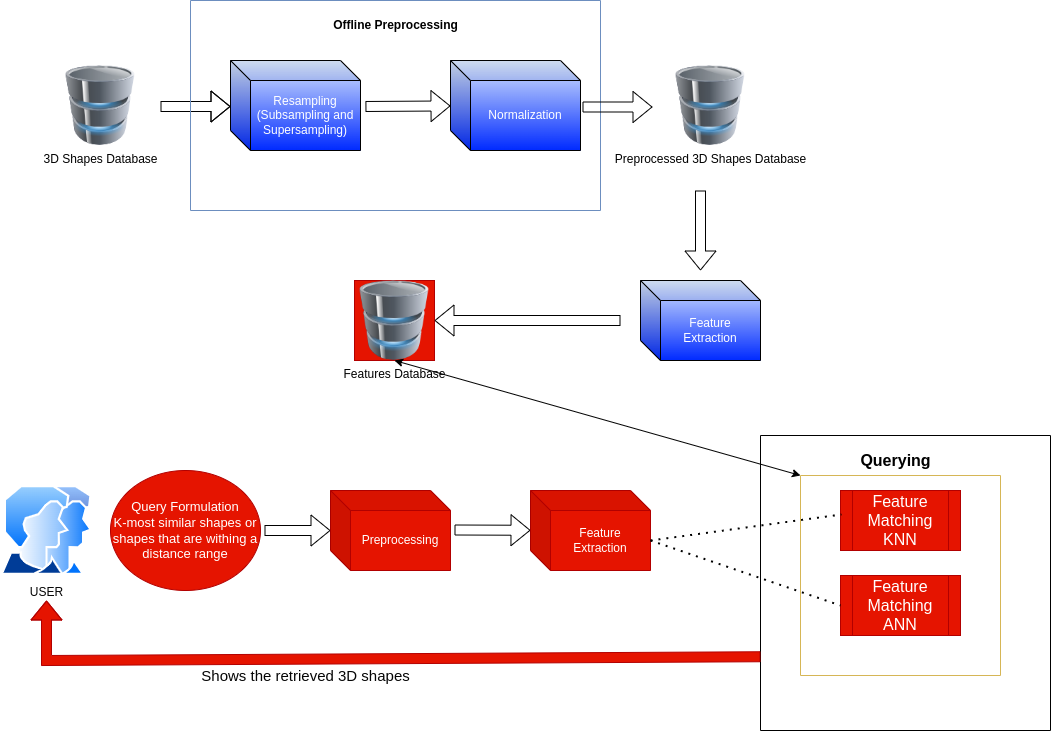
\includegraphics[width=0.9\textwidth]{assets/pipeline.png}
    \caption{Multimedia retrieval system pipeline}
    \label{fig:mr-pipeline}
\end{figure}

\begin{table}
    \caption{Global Notations}
    \centering
    \resizebox{\textwidth}{!}{
        \begin{tabular}{|c|c|c|c|}
            \hline
            Name & Notation & Description & Formula \\ [0.5ex]
            \hline\hline

            \newtag{3D Point}{3d_point_not} & $p$ & A tuple representing coordinates in 3D & $p = (x,y,z)$ \\
            \hline
            
            \newtag{Normal}{normal_not} & $|| \cdot ||$ & The distance from the origin & $||p|| = \sqrt{p_x^2 + p_y^2 + p_z^2}$ \\
            \hline      
            
            \newtag{Triangle}{triangle_not} & $\mathcal{T}$ & A set of 3 points forming a triangle & $\mathcal{T} = \{p_1, p_2, p_3\}$ \\
            \hline

            \newtag{Tetrahedron}{tetrahedron_not} & $\mathcal{T}h$ & A set of 4 points forming a tetrahedron & $\mathcal{T}h = \{p_1, p_2, p_3, p_4\}$ \\
           \hline
           \newtag{Tetrahedron with}{tetrahedron_origin_not} & \multirow{2}{*}{$\mathcal{T}h_O$} & A set of 3 points forming a tetrahedron  & \multirow{2}{*}{$\mathcal{T}h_O = \{p_1, p_2, p_3, O\}$} \\
              a vertex in origin & & where the 4th point is the origin $O = (0,0,0)$ & \\
          \hline
            
           \newtag{Triangle center}{triangle_center_not} & $\mathbf{C}_{\mathcal{T}}$ & The center of the triangle & $\mathbf{C}_{\mathcal{T}} = (\frac{p_{1_x} + p_{2_x} + p_{3_x}}{3}, \frac{p_{1_y} + p_{2_y} + p_{3_y}}{3}, \frac{p_{1_z} + p_{2_z} + p_{3_z}}{3} )$ \\
           \hline      
            
           Unsigned tetrahedron & \multirow{2}{*}{\newtag{$Vol_{\mathcal{T}h}$}{tetrahedron_volume_not}} & \multirow{2}{*}{The volume of the tetrahedron $\mathcal{T}h$} & \multirow{2}{*}{$Vol_{\mathcal{T}h} = \frac{1}{6} \cdot (p_1 - p_4) \cdot ((p_2 - p_4) \times (p_3 - p_4))$} \\
           volume & & & \\
           \hline   
            
           Triangle area & \newtag{$A_{\mathcal{T}}$}{triangle_area_not} & The area of the triangle $\mathcal{T}$ & $A_{\mathcal{T}} = \frac{1}{2} \cdot ||(p_2 - p_1) \times (p_3 - p_1)|| $ \\
           \hline   
            
           Vertices & \newtag{$V$}{vertices_not} & A set of 3D points & $V = \{v_1, ..., v_N\}$ \\
           \hline      
             
           Faces & \newtag{$F$}{faces_not} & A set of triples of indexes & $F = \{(i,j,k), ..., (l,m,n)\}$ \\
           \hline      
            
           \multirow{2}{*}{Shape} &\multirow{2}{*}{\newtag{$\mathcal{S}$}{shape_not}} & A set of vertices and a set of & \multirow{2}{*}{$\mathcal{S} = (V_\mathcal{S}, F_\mathcal{S})$} \\
           & & faces containing vertices indexes & \\
           \hline      
            
            Barycenter & \newtag{$b_{\mathcal{S}}$}{barycenter_not} & The geometric center of shape $\mathcal{S}$ & $b_{\mathcal{S}} = \frac{1}{N} \sum_{i=1}^N \mathbf{C}_{\mathcal{T}_i} \cdot A_{\mathcal{T}_i}$  \\
           \hline      

           \multirow{2}{*}{\newtag{All the matrices}{matrices_class_not}} & \multirow{4}{*}{$\mathbb{M}_{n,m}(\cdot)$} & e.g. $\mathbb{M}_{2,3}(\mathbb{R})$ represents & \multirow{4}{*}{$\mathbb{M}_{n,m}(\cdot) = 
            \begin{pmatrix}
                a_{1,1} & \cdots & a_{1,m} \\
                \vdots & \ddots & \vdots \\
                a_{n,1} & \cdots & a_{n,m} \\
            \end{pmatrix}
           $} \\
           & & all the matrices & \\
           \multirow{2}{*}{of size $n \times m$} & & with 2 rows and 3 columns & \\
           & & containing only real numbers & \\
           \hline
            
           \newtag{Identity Matrix}{identity_matrix_not} & $\mathbb{I}_N$ & The $N\times N$ identity matrix & 
            
           $\mathbb{I}_N = 
             \begin{pmatrix}
                  1 & 0 &\cdots & 0 \\
                  0 & 1 &\cdots & 0 \\
                 \vdots &\vdots& \ddots & \vdots \\
                 0 & 0 & \cdots & 1
             \end{pmatrix}$ \\
           \hline      
            
           \newtag{Matrix transposition}{matrix_transposition_not} & $(\cdot)^T$ & Transposing a matrix & Let $A=(a_{i,j})$ then $A^T=(a_{j,i})$\\
           \hline

           \newtag{Covariance}{cov_x_y_not} & \multirow{3}{*}{$cov(x,y)$} & An indicator of the spread of the vertices & $cov(x,y) = \frac{1}{N-1} \sum_{i=1}^N (x_i - \bar{x}) \cdot (y_i - \bar{y})$, \\
           of $x$ coordinate & & along $x$ coordinate axis & where $\bar{x} = \frac{1}{N} \sum_{i=1}^N x_i$\\
           w.r.t. $y$ coordinate & & w.r.t. the spread along the $y$ axis & $\bar{y} = \frac{1}{N} \sum_{i=1}^N y_i$ \\
           \hline      
            
           \newtag{Covariance matrix}{cov_shape_not} & \multirow{3}{*}{$Cov(V_{\mathcal{S}})$} & The matrix describing the spread & \multirow{3}{*}{ $Cov(V_{\mathcal{S}}) = \begin{pmatrix}
                    cov(x,x) & cov(x,y) & cov(x,z)\\
                    cov(y,x) & cov(y,y) & cov(y,z)\\
                    cov(z,x) & cov(z,y) & cov(z,z)\\ 
              \end{pmatrix}$}
              \\
            of shape $\mathcal{S}$ & & of vertices w.r.t. coordinate axes & \\
            & & & \\
           \hline      
            
           \newtag{Eigenvalue}{eigval_shape_not} & \multirow{2}{*}{$\lambda$} & The variability of the data in the direction & \multirow{2}{*}{$det(Cov(V_{\mathcal{S}}) - \lambda \cdot \mathbb{I}_N) = 0$} \\
           of shape $\mathcal{S}$ & & corresponding to the eigenvectors & \\
           \hline      
            
           \newtag{Eigenvector}{eigvec_shape_not} & \multirow{2}{*}{$v_{\lambda}$} & The direction vectors in which & \multirow{2}{*}{$Cov(V_{\mathcal{S}}) \cdot \overrightarrow{v_{\lambda}} = \lambda \cdot \overrightarrow{v_{\lambda}}$} \\
           of shape $\mathcal{S}$ & & the data is spread the most & \\
           \hline      
            
           Flipping axis & \multirow{3}{*}{\newtag{$f_i$}{flip_axis_not}} & The weighted difference & \multirow{2}{*}{$f_i = \sum\limits_{j=1}^M  sign({C}_{\mathcal{T}_j}^i) \cdot ({C}_{\mathcal{T}_j}^i)^2$} \\
           component & & of the amount of vertices & \\
            of shape $\mathcal{S}$ & & on the positive and negative side of axis $i$ & where $|F_{\mathcal{S}}| = M$ \\ 
           \hline      
            
           Re-scaling & \multirow{2}{*}{\newtag{$\sigma_{unit}(\mathcal{S})$}{rescale_not}} & The unit cube re-scaling factor & $\sigma_{unit}(\mathcal{S}) = \frac{1}{m}$\\
           unit cube factor & & of a shape $\mathcal{S}$ & $m = max(|x_{max} - x_{min}|, |y_{max} - y_{min}|, |z_{max} - z_{min}|)$ \\ 
           \hline
           
           \multirow{2}{*}{\newtag{LP norm}{lp_norm}} & \multirow{2}{*}{$L_p(\cdot, \cdot)$} & \multirow{2}{*}{A distance function between two vectors} & $L_p(\overrightarrow{x},\overrightarrow{y}) = \left( \sum_{i = 1}^n \left| x_i - y_i \right| ^p \right)^{\frac{1}{p}}$ \\
           & & & $L_{\infty}(\overrightarrow{x},\overrightarrow{y}) = \max_{i = 1}^n \left| x_i - y_i \right|$ \\
           
           \hline
           \newtag{Cosine distance}{cos_dist} & $d_{cos}(\cdot, \cdot)$ & A distance function between two vectors& $d_{cos}(\overrightarrow{x}, \overrightarrow{y}) = 1 - \frac{\overrightarrow{x} \cdot \overrightarrow{y}}{||\overrightarrow{x}||\cdot ||\overrightarrow{y}||}$ \\
           
            \hline
            \multirow{2}{*}{\newtag{Mahalanobis Distance}{mahalanobius_dist}} & \multirow{2}{*}{$d_{mahalanobis}(\cdot, \cdot)$} & \multirow{2}{*}{A distance function between two vectors}  & $d_{mahalanobis}(\overrightarrow{x}, \overrightarrow{y}) = \sqrt{(\overrightarrow{x} - \overrightarrow{y})^T Cov^{-1}(X) (\overrightarrow{x} - \overrightarrow{y})}$\\
            & & & where $X$ is the set of all points in the space \\
            \hline
           
            \multirow{4}{*}{\newtag{Earth's Mover's Distance}{emd_dist}} & \multirow{4}{*}{$emd(\cdot,\cdot)$} & \multirow{2}{*}{A distance function} & $emd(A,B) = \min\limits_{F} \frac{\sum_{i=1}^{n} \sum_{j=1}^{m} f_{i, j} d_{i, j}}{\sum_{i=1}^{n} \sum_{j=1}^{m} f_{i,j}}$ \\
            & & & where $F=\{f_{i,j}\}$, with $f_{i,j}$ \\
            & & \multirow{2}{*}{between two histograms} & the flow between bin $i$ of $A$ and bin $j$ of $B$ \\
            & & & and $d_{i,j}$ the distance between the bins (see \cite{rubner_emd_2000})\\
            \hline
            
            \multirow{4}{*}{\newtag{Kullback-Leibler Divergence}{KL_dist}} & \multirow{4}{*}{$d_{KL}(\cdot, \cdot)$} & \multirow{2}{*}{A distance function between} & $d_{KL}(A, B) = \sum_{i=1}^n (a_i - b_i) \log \left( \frac{a_i}{b_i} \right)$ \\
            & & & where $A$ and $B$ are discrete random variables\\
            & & \multirow{2}{*}{two probability distributions} & where the probability of the event $i$ equals to \\
            & & & $a_i$ and $b_i$ respectively (see \cite{kullback1951information})\\
            \hline
            
        \end{tabular}
    }
    \label{tab:notations}
\end{table}
Table \ref{tab:notations} describes all notations used throughout the report. We use the notation $\overrightarrow{p_1} \times \overrightarrow{p_2}$ for the cross product between two vectors; $\alpha \cdot \overrightarrow{p_1}$ for scalar multiplication; $\overrightarrow{p_1} \cdot \overrightarrow{p_2}$ for dot product; and $A \cdot B$ for matrix multiplication. Table \ref{tab:code_tools} presents all the dependent libraries of our system.

\begin{table}
    \caption{Code Tools}
    \centering
    \resizebox{\textwidth}{!}{
        \begin{tabular}{|c|c|c|c|}
            \hline
            Name & Description & Citation/Website \\
            [0.5ex]
            \hline\hline
                \newtag{Python 3}{python_t} &
                Base programming language for the project &
                \cite{10.5555/1593511} \\
            \hline
                \newtag{PyMeshLab}{pymeshlab_t} & 
                Python interface to \ref{meshlab_t} &
                \cite{pymeshlab} \\
            \hline
                \newtag{MeshLab}{meshlab_t} &
                System for processing and editing 3D shapes &
                \cite{MeshLab} \\
            \hline
                \newtag{PyVista}{pyvista_t} &
                Visualisation of 3D Models &
                \cite{sullivan2019pyvista} \\
            \hline
                \multirow{2}{*}{\newtag{Numba}{numba_t}} &
                Speed up (some) \ref{python_t} \& \ref{np_t} functions &
                \multirow{2}{*}{\cite{lam2015numba}} \\
                & by translating them into machine code & \\
            \hline
                \newtag{NumPy}{np_t} &
                Extensive mathematical functions for \ref{python_t}, computed quickly &
                \cite{harris2020array} \\
            \hline
                \newtag{SciPy}{scipy-t} & 
                Fundamental algorithms for scientific computing &
                \cite{2020SciPy-NMeth} \\
            \hline
                \newtag{Matplotlib}{plt_t} &
                Plotting data for visualisation purposes; plots used in the report &
                \cite{Hunter:2007} \\
            \hline
                \newtag{SciencePlots}{sciplots_t} & 
                Scientific plot styles for \ref{plt_t} &
                \href{https://pypi.org/project/SciencePlots/}{pypi.org} \\
            \hline
                \newtag{PySimpleGUI}{PySimpleGUI_t} &
                Used to make the GUI for the end system &
                \href{https://www.pysimplegui.org/}{pysimplegui.org} \\
            \hline
                \newtag{Annoy}{Annoy_t} & Used to compute an index of the feature database & \href{https://pypi.org/project/annoy/1.0.3/}{pypi.org}
                \\
            \hline
        \end{tabular}
    }
    \label{tab:code_tools}
\end{table}

 
\newpage
\section{Introduction}
\label{section:introduction}
In this report, we describe our implementation of a 3D shape retrieval system which aims to return the shapes that are most similar to a user-given example.
Figure \ref{fig:mr-pipeline} presents a pipeline of our system.
The processes coloured in blue are performed offline, whilst the ones coloured in red are performed online (i.e.\ when a query is made).

This report is structured as follows, in Section \ref{section:setting-the-environment} we describe technical details about the environment we use to develop this system such as the dataset and libraries we use.
Section \ref{section:preprocessing} describes how we preprocess the shapes from the dataset.
In Section \ref{section:feature-extraction}, we describe what features we use in order to discriminate the shapes.
The approaches to computing the distance/dissimilarity between the shapes are presented and described in Section \ref{section:discriminating-using-features}.
Two approaches that help to reduce the complexity of the computations, allowing for scalability of our system for bigger data sets, are described in Section \ref{section:scalability}.
Section \ref{section:retrieval-system} brings a brief overview along with instructions on how to use our system from a user perspective.
A quantitative evaluation of our system is presented in Section \ref{section:evaluation} along with discussions regarding how well the system performs for different shapes.
The report ends with Section \ref{section:conclusions}, in which we discuss the strong and weak points of the system, as well as give directions for further development.

\section{Setting up the Environment}
\label{section:setting-the-environment}
In this section, we describe the environment setup that we use for developing our 3D shape retrieval system.
Python version 3.9 is the programming language in which the system is developed.
The reason for this choice is the rich assortment of Python libraries for 3D mesh manipulation, processing and
visualization - you can see our selection of them in \ref{tab:code_tools}, as well as our familiarity with the langauge.
The code for this project is available on the following  \href{https://github.com/cristi2019255/MultimediaRetrieval}{GitHub repository}.

\subsection{Dataset}
The dataset of 3D models we use for this project is a combination of the Princeton Shape
Benchmark \cite{Princeton} and the labeled PSB dataset \cite{PSB_dataset,PSB_paper}.
These datasets consist of a set of files in which the positions of vertices of the 3D shape are listed, along with a
set of indices describing the faces of the shape.
The shapes in this dataset are stored mostly in \verb!.off! and \verb!.obj! files.
However, we want to design a system that deals with all present kinds of file extensions for storing 3D objects.
Therefore, we convert \verb!.off! and \verb!.obj! files into \verb!.ply! files using a PyMeshLab \href{https://pymeshlab.readthedocs.io/en/latest/classes/meshset.html}{MeshSet class}.

In total, our final database has {} shapes.
\subsection{Database}
During the development of our retrieval system, one of the tasks we do is computing shape features and storing them
for all shapes in our dataset.
For this purpose and for ease of collaboration among the developers' team we chose to use a PostgreSQL database
hosted by Heroku (see the \href{https://github.com/cristi2019255/MultimediaRetrieval}{GitHub repository} for more
details).
This cloud database contains all relevant information of the shapes in the datasets that we use.
It contains for example the relative filepath for the 3D model, global information about the meshes such as the
amount of vertices and faces, and of course the features for the feature vector are stored there.
The data stored in this big cloud database will be inserted once after the preprocessing and feature extraction steps.
Once this is done, the querying for similar shapes can be done on the data that is stored there.

\subsection{Viewing 3D Models}
The visualization of the shapes is done using the PyVista library which has easy-to-use functions for loading and
displaying files, which can also be paired up with a custom theme.
For visualization, a list of files is passed to the function, and a new window is opened containing the faces and edges of the shape.
The window allows manipulation of the view of the visualization by zooming in, rotating, and moving the visualised
shape(s).
Additionally, the file name \& relative path are displayed above their respective figures.
An example of the visualization of two shapes from the dataset can be seen in Figure \ref{fig:initial}.

\begin{figure}[ht]
  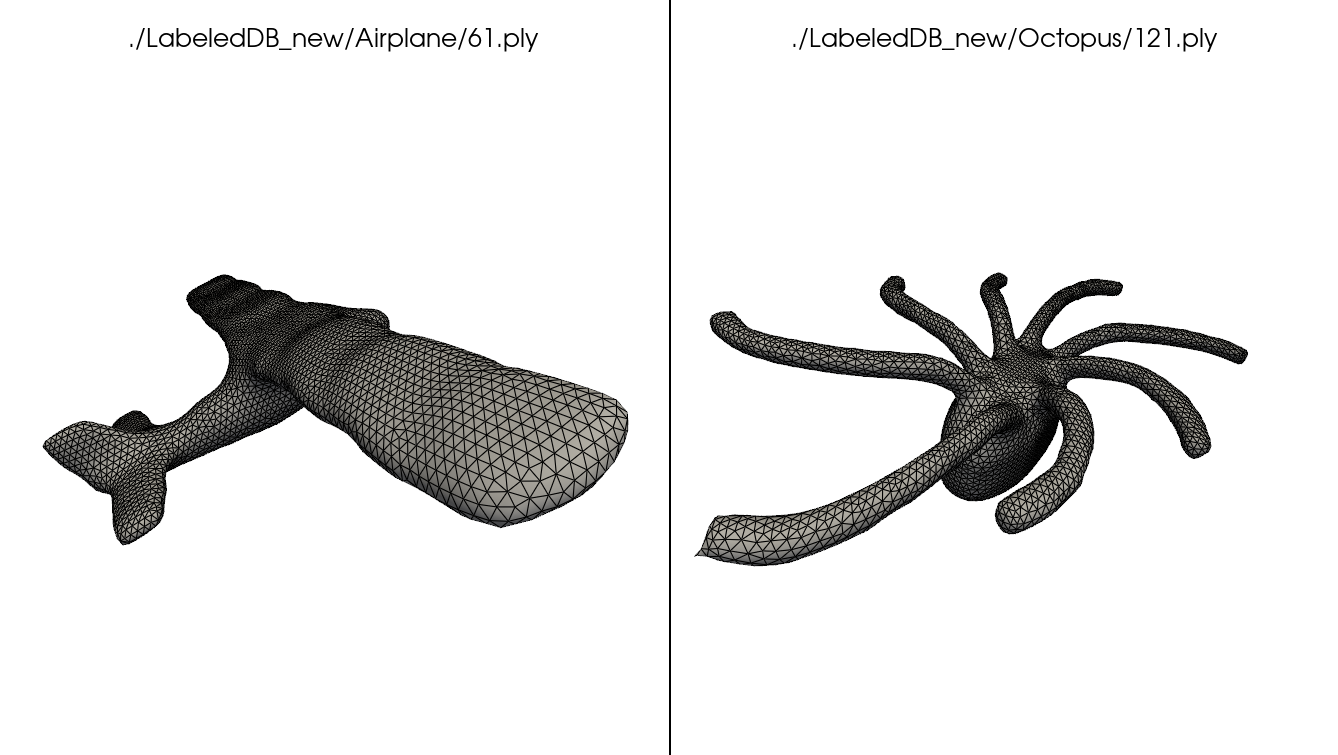
\includegraphics[width=\linewidth]{assets/visualisation/shapes_initial.png}
  \caption{Example of 3D mesh visualisation using PyVista. Models for an airplane and an octopus are visualised. The view of the models (size, rotation, position) can be modified.}
  \label{fig:initial}
\end{figure}


\section{Preprocessing}
\label{section:preprocessing}
Before we can perform any kind of feature extraction over the 3D shapes, we first have to prepare our data set so that the shapes are resampled and normalized.
We want all the shapes in our data set to have approximately the same number of faces and vertices.
The reasoning behind this is that in the feature extraction step, we would like to compute fixed-size feature vectors
using local descriptors, and allowing for shapes that differ by orders of magnitude in the number of vertices and
number of faces might lead to inaccurate features between different shapes.
Aside from the same number of faces and vertices, we would also like to compute features that are invariant with
respect to the rotation or scale of a shape.
In order to achieve this we transform the data set shapes such that after a series of such transformations all the
shapes have the following properties:
\begin{itemize}
    \item the barycenter of the shape is in the origin of the coordinate space;
    \item the shapes are re-scaled to the unit cube;
    \item the shapes are aligned such that the most spread of the shape is along the $x$ coordinate axis, the medium spread is aligned along the $y$-axis and the minimal spread is aligned along the $z$-axis;
    \item the shape is concentrated on the positive side of each plane $x = 0, y = 0, z = 0 $. 
\end{itemize}


\subsection{Analysing a Single Shape}
The preprocessing step involves getting certain information about the shapes, detecting the ones which are not
quality-compliant, and then preprocessing them in such a way that they fit our requirements.
This section will discuss our approach to doing this.

For the preprocessing stage, the information we track for each shape is the number of vertices, number of faces, the
type of faces (triangles/squares/mixed), and the axis-aligned bounding box of the shape.

Getting this information is largely done via methods that are already implemented in PyMeshLab.
The number of vertices and faces are accessed with the \verb!vertex_number()! and \verb!face_number()! methods
respectively.
The type of faces for a given shape is determined by the number of points $p$ in a face $f = (p_1, ..., p_n)$ belonging to the set of faces \ref{faces_not}.
If, for all $f \in$ \ref{faces_not}; $n = 3$, the shape is constructed of triangles;
if $n = 4$ for all $f \in$ \ref{faces_not}, the shape is constructed of quads (rectangular polygons);
if some $n = 3$ and some $n = 4$, then it is a mixed shape.
The bounding box is extracted via the \verb!bounding_box()! method, and then aligned along each dimension $x, y, z$ and the diagonal of the shape.

Two examples of the output of this analysis and the respective visualisations of the shape are shown in Figure
\ref{fig:analysed}.
The shapes we chose are the two that have a number of faces and vertices which is closest to the respective average
in the dataset.
Notice that the number of vertices, faces, their type, and the coordinates of the bounding box are shown below the meshes.

\begin{figure}[ht]
    \centering
    \begin{subfigure}{0.45\textwidth}
        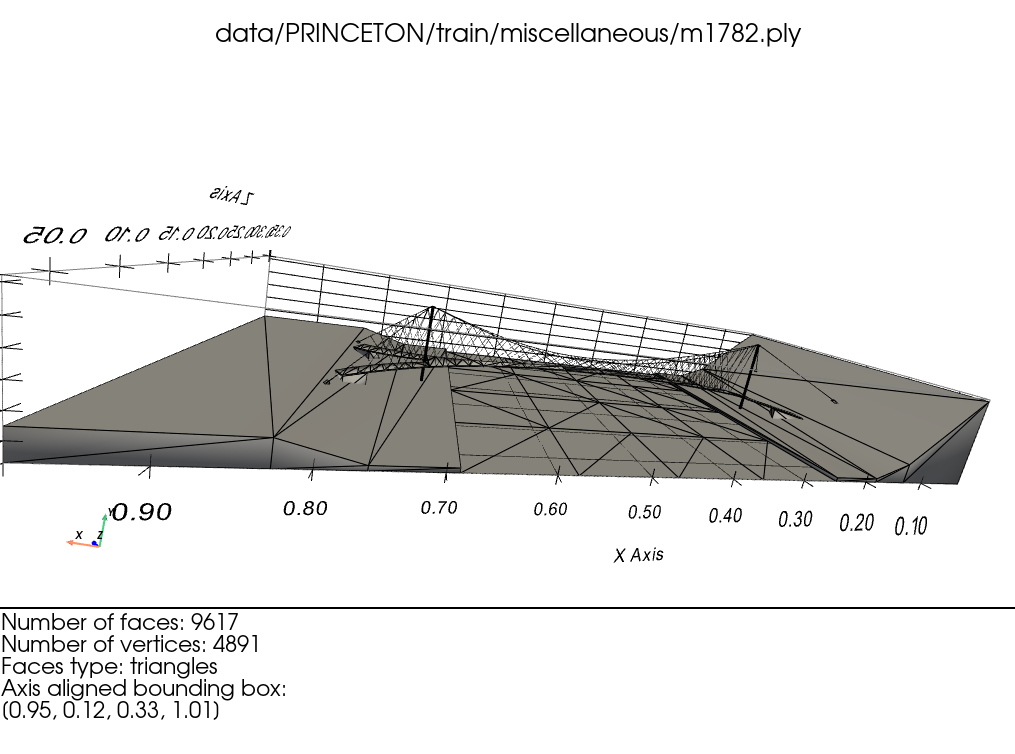
\includegraphics[width=\textwidth]
        {assets/visualisation/faces_avg_shape.png}
        \caption{Model with number of faces closest to the average number of faces}
    \end{subfigure}
    \hfill
    \begin{subfigure}{0.45\textwidth}
        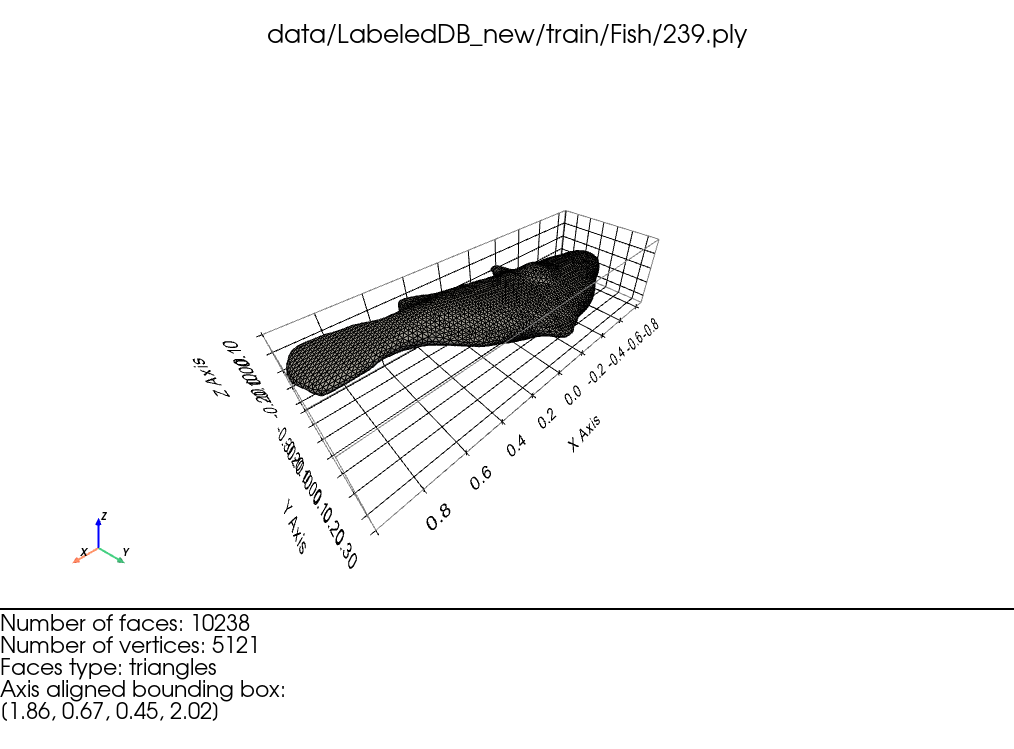
\includegraphics[width=\textwidth]
        {assets/visualisation/vertices_avg_shape.png}
        \caption{Model with number of vertices closest to the average number of vertices}
    \end{subfigure}
    \caption{Visualisation with the number of vertices, number of faces, faces type and the bounding box computed.}
    \label{fig:analysed}
\end{figure}

\subsection{Statistics Over the Whole Database}
As we will see in one of the following subsections, the normalisation process does not require any decisions or user-defined parameters.
This is not the case however in the resampling step, where we have to decide on a few variables.
One of these is the number of faces (or, by proxy, number of vertices) we want the shapes in our database to be made up of.
This subsection presents statistics about our data set along with reasoning for the design choices we made in creating the resampling process.

In order to understand our dataset, we first perform a class distribution analysis in which we compute the distribution of the shapes in the data set over the class labels.
The results are presented in Figure \ref{fig:class-distribution}.
Observe that the shapes are not uniformly distributed.
For instance, we have 200 objects in the vehicle class and only 20 in classes like Bust, Hand, Bird, etc.
However, this is not a problem for the system we develop.


In Figure \ref{fig:statistics-faces-vertices-number} we present the distribution over the number of faces and number of vertices of the shapes.

Since we would like to make our system independent of the data set and, more importantly, we would like our system to work quickly, we decided to resample the shapes such that, for each shape \ref{shape_not}, \ref{faces_not}=5000.
In choosing the value for this number, we considered firstly what it will be used for - computing descriptive features of the shapes.
A higher value gives more accurate results, but requires (much) more computation.
For many features, the $\mathcal{O}$ computation is dependant, in some way, on the number of \ref{faces_not}.
However, having a value that is too low would result in features which are very inaccurate for the original shape that we are trying to describe.
$5000$ is a good compromise between these two factors, as well as a good heuristic approximation to the usual number of faces we believe a 3D shape will have.

\begin{figure}
    \centering
    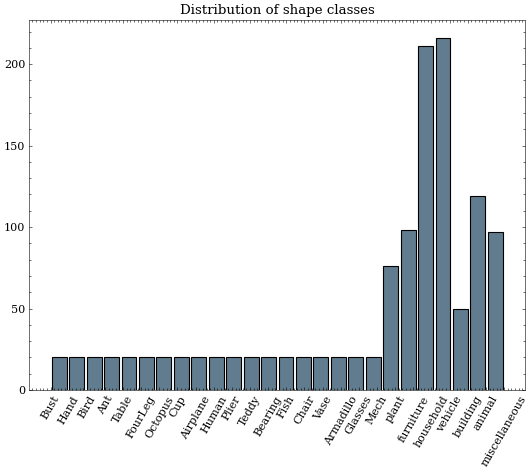
\includegraphics[width = 0.8\textwidth]{assets/preprocessing/Distribution_of_shape_classes.png}
    \caption{Distribution of shape classes}
    \label{fig:class-distribution}
\end{figure} 

\begin{figure}
    \centering
    \begin{subfigure}[b]{0.45\textwidth}
         \centering
         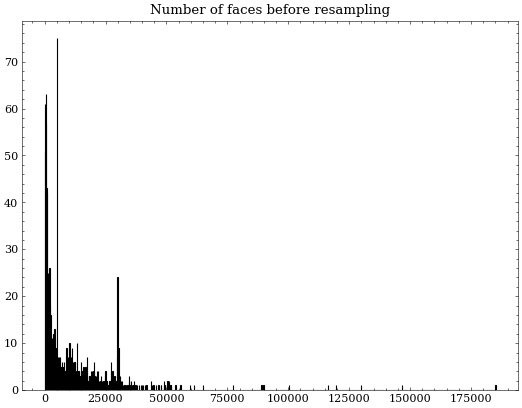
\includegraphics[width=\textwidth]{assets/preprocessing/Number_of_faces_before_resampling.png}
         \caption{Distribution of the number of faces}
         \label{fig:statistics-faces-vertices-number-a}
     \end{subfigure}
     \hfill
     \begin{subfigure}[b]{0.45\textwidth}
         \centering
         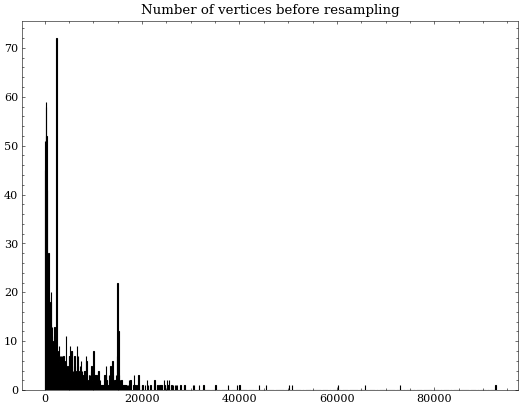
\includegraphics[width=\textwidth]{assets/preprocessing/Number_of_vertices_before_resampling.png}
         \caption{Distribution of the number of vertices}
         \label{fig:statistics-faces-vertices-number-b}
     \end{subfigure}
    \caption{Statistics for resampling decisions}
    \label{fig:statistics-faces-vertices-number}
\end{figure}

\subsection{Sub-Sampling and Super-sampling}
The 3D meshes of the shapes we are working with have a different number of faces and vertices, as can be seen in
Figure \ref{fig:statistics-faces-vertices-number}.
In order to compare these shapes with each other fairly, we first have to manipulate these meshes such that these
amounts are roughly the same between shapes.
That way, the features that will eventually be extracted, will be meaningful to us and our shape retrieval system -
at the end of the day, we want to compare the shapes to each-other, and that can only be done fairly if they have a
similar granularity.
As we mentioned earlier, we have chosen to resample the meshes such that the number of faces comes near the predefined
number of $5000$ faces.
If shapes have a higher number of faces, then we have to lower this amount.
Whenever the amount of faces is very low compared to $5000$, then we have to somehow increase the number of faces.
This is done by respectively sub-sampling and super-sampling the 3D meshes.
In this subsection we explain how exactly we implemented this.

As discussed in our environment setup, PyMeshLab offers extensive functionality for performing operations on meshes.
It offers a wide range of so-called filters for many tasks, such as mesh manipulation and processing.
Among these filters, there is a selection of several algorithms which can be used for re-meshing 3D meshes.

\paragraph{Sub-sampling}
For sub-sampling, we use the following configuration:
\begin{itemize}
    \item the ``Meshing Decimation Quadric Edge Collapse'' filter. This filter simplifies the mesh to a mesh with a
    specific target amount of faces lower than the original amount of faces;
    \item a target amount of faces, which we have set to $5000$, the wanted amount of faces;
    \item a quality threshold of $1$, which is the other parameter for this filter. This value penalizes bad shaped faces maximally. Thus, we try to keep the original surface of the shape as intact as possible.
\end{itemize}

In Figure \ref{fig:resampled_woman}, an example of the sub-sampling results is shown.
In it, we compare the original mesh of a model of a woman to its processed, sub-sampled, mesh.
Very detailed parts of the 3D model - such as the face, shoes, legs and hands, lose a lot of information, but they
still maintain the overall shape of the original mesh in those specific parts.
The areas of the resulting faces are also very comparable after sub-sampling, whereas the faces in the original mesh
had faces of varying sizes.
In fine-grained areas, such as the shoes of the model, there were some very small faces, while the dress for example
has faces with a fairly large area in comparison to those.
Again, this is to be expected, since more triangles are needed to model the finer details of the models.

\begin{figure}[ht]
  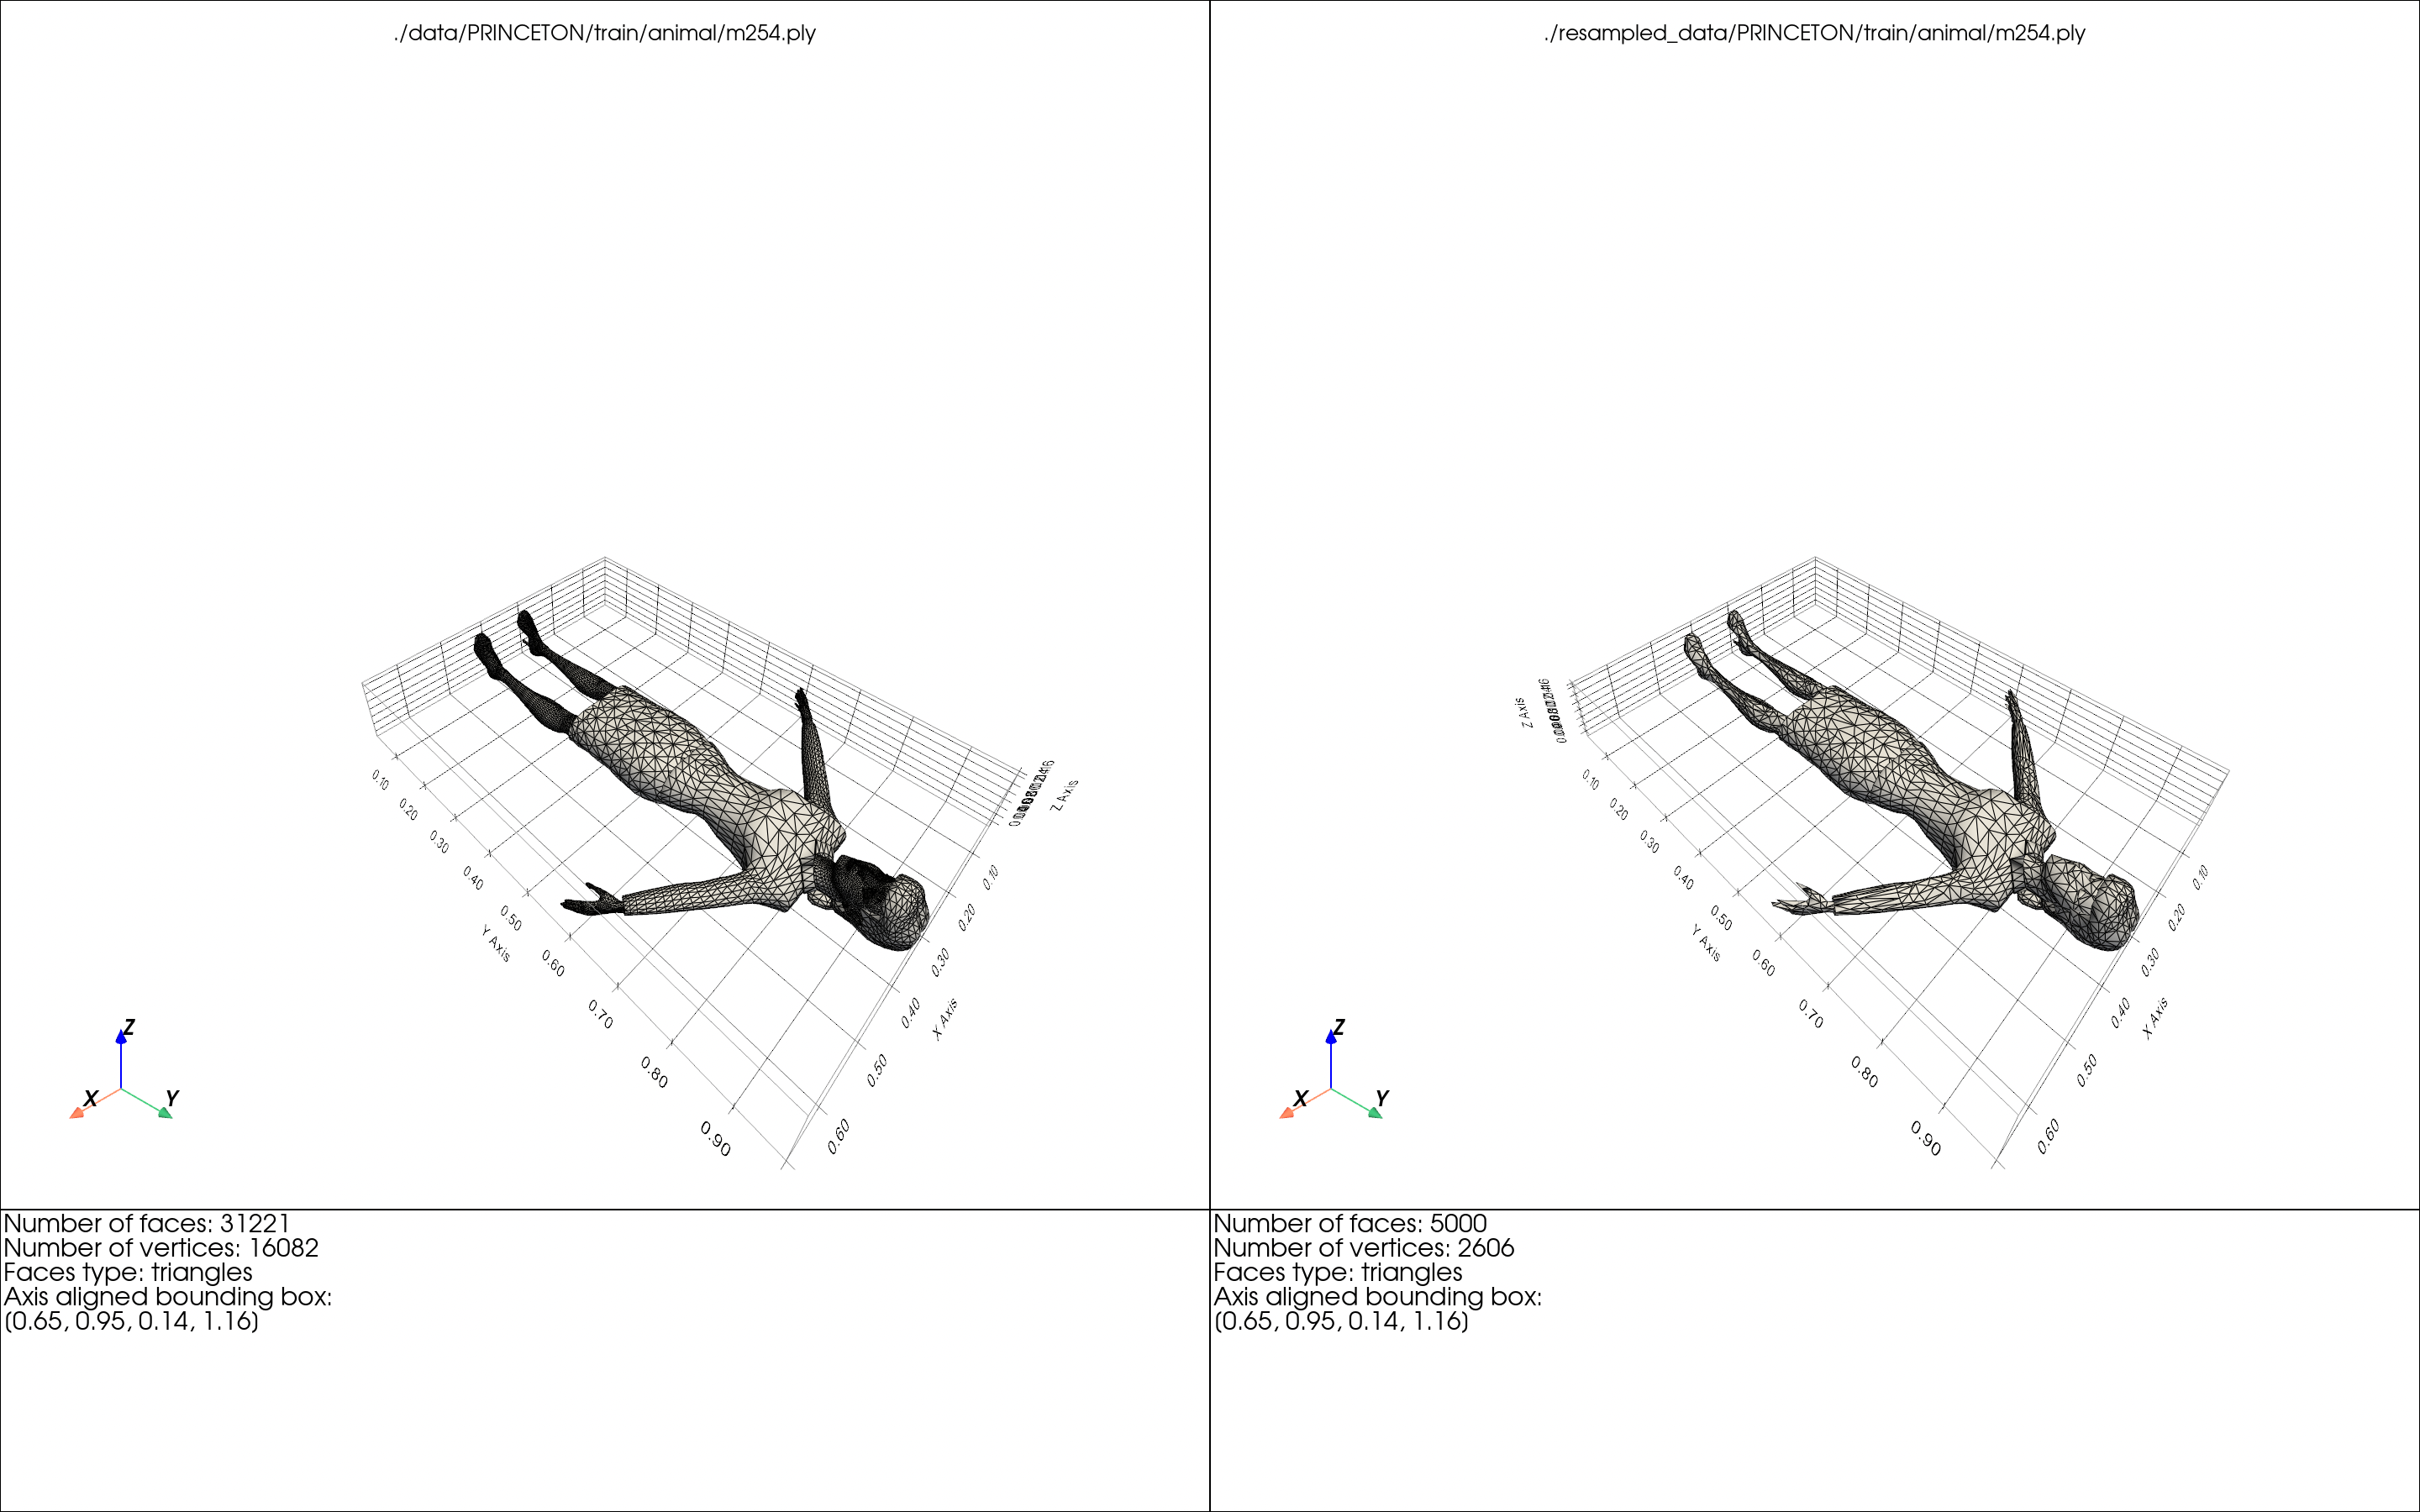
\includegraphics[width=\linewidth]
  {assets/preprocessing/resampling/woman_resampled.png}
  \caption{Comparison of the original 3D mesh of a woman on the left with its resulting sub-sampled mesh on the right.}
  \label{fig:resampled_woman}
\end{figure}

\paragraph{Super-sampling}
When we have to perform super-sampling on a mesh with a low number of faces, we are currently using the ``Meshing
Surface Subdivision Midpoint'' filter.
This filter splits each edge on its midpoint, creating a new set of faces, each of which is constructed in the
interior of the original face.
Since our database consists of 3D meshes that only have triangles as faces, every triangle face is replaced by the four triangle faces that can be formed in its interior.
Thus, every iteration of this algorithm multiplies the number of faces of the model by $4$.
Knowing this, we can calculate the exact number of iterations needed to reach (at least) the target amount of $5000$
faces.
This proves very useful as one of the required parameters for the subdivision algorithm implementation in PyMeshLab is
the number of iterations.
The implementation of super-sampling using this filter is somewhat more involved than for the sub-sampling.
The pipeline for our super-sampling implementation is as follows:
\renewcommand{\labelenumii}{\theenumii}
\renewcommand{\theenumii}{\theenumi.\arabic{enumii}.}
\begin{enumerate}
    \item Perform the subdivision algorithm to reach $5000$ or more faces, given the number of iterations needed.
    \item If the algorithm raises an error:
    \begin{enumerate}
        \item Try to repair the mesh with the ``Meshing Repair Non-Manifold Edges'' filter.
        \item If the repair is successful, try to perform the subdivision algorithm on the repaired mesh.
    \end{enumerate} 
    \item If the number of faces exceeds the wanted amount of faces, call the sub-sampling functionality described
    above to achieve exactly the target number of faces.
\end{enumerate}

%We provide this iteration amount as an argument to the filter to obtain a mesh with $5000$ faces or more. If the amount of faces exceeds $5000$ we use the sub-sampling to make sure that the target amount of faces is exactly $5000$.
As seen in step 2 of the workflow, the subdivision algorithm might fail if a mesh is not 2-manifold, i.e.\ if it
contains holes.
To account for this, we have implemented functionality that attempts to repair the mesh.
If the mesh is successfully repaired, we try to run the subdivision algorithm on the repaired mesh as necessary.
For the repairing of a mesh, we use the ``Meshing Repair Non-Manifold Edges'' filter.
Using this filter, we have the option of either removing the smallest area faces until the mesh becomes 2-manifold,
or splitting vertices in such a way that each non-manifold edge-chain will become a border.
The default behavior is to remove the faces with the smallest area, which is what we chose.
Finally, after the super-sampling is performed, we re-use the sub-sampling implementation to get meshes with exactly
$5000$ faces.

An example of the super-sampling process can be seen in Figure \ref{fig:resampled_castle}.
Here, a comparison is made between the original mesh of the 3D shape of a castle and a super-sampled version of this
mesh.
This comparison shows that the super-sampling happens quite uniformly, which is not trivial and very satisfactory for
us.
The resulting mesh is practically identical to the original mesh, with the difference of having $5000$ faces.

\begin{figure}[ht]
  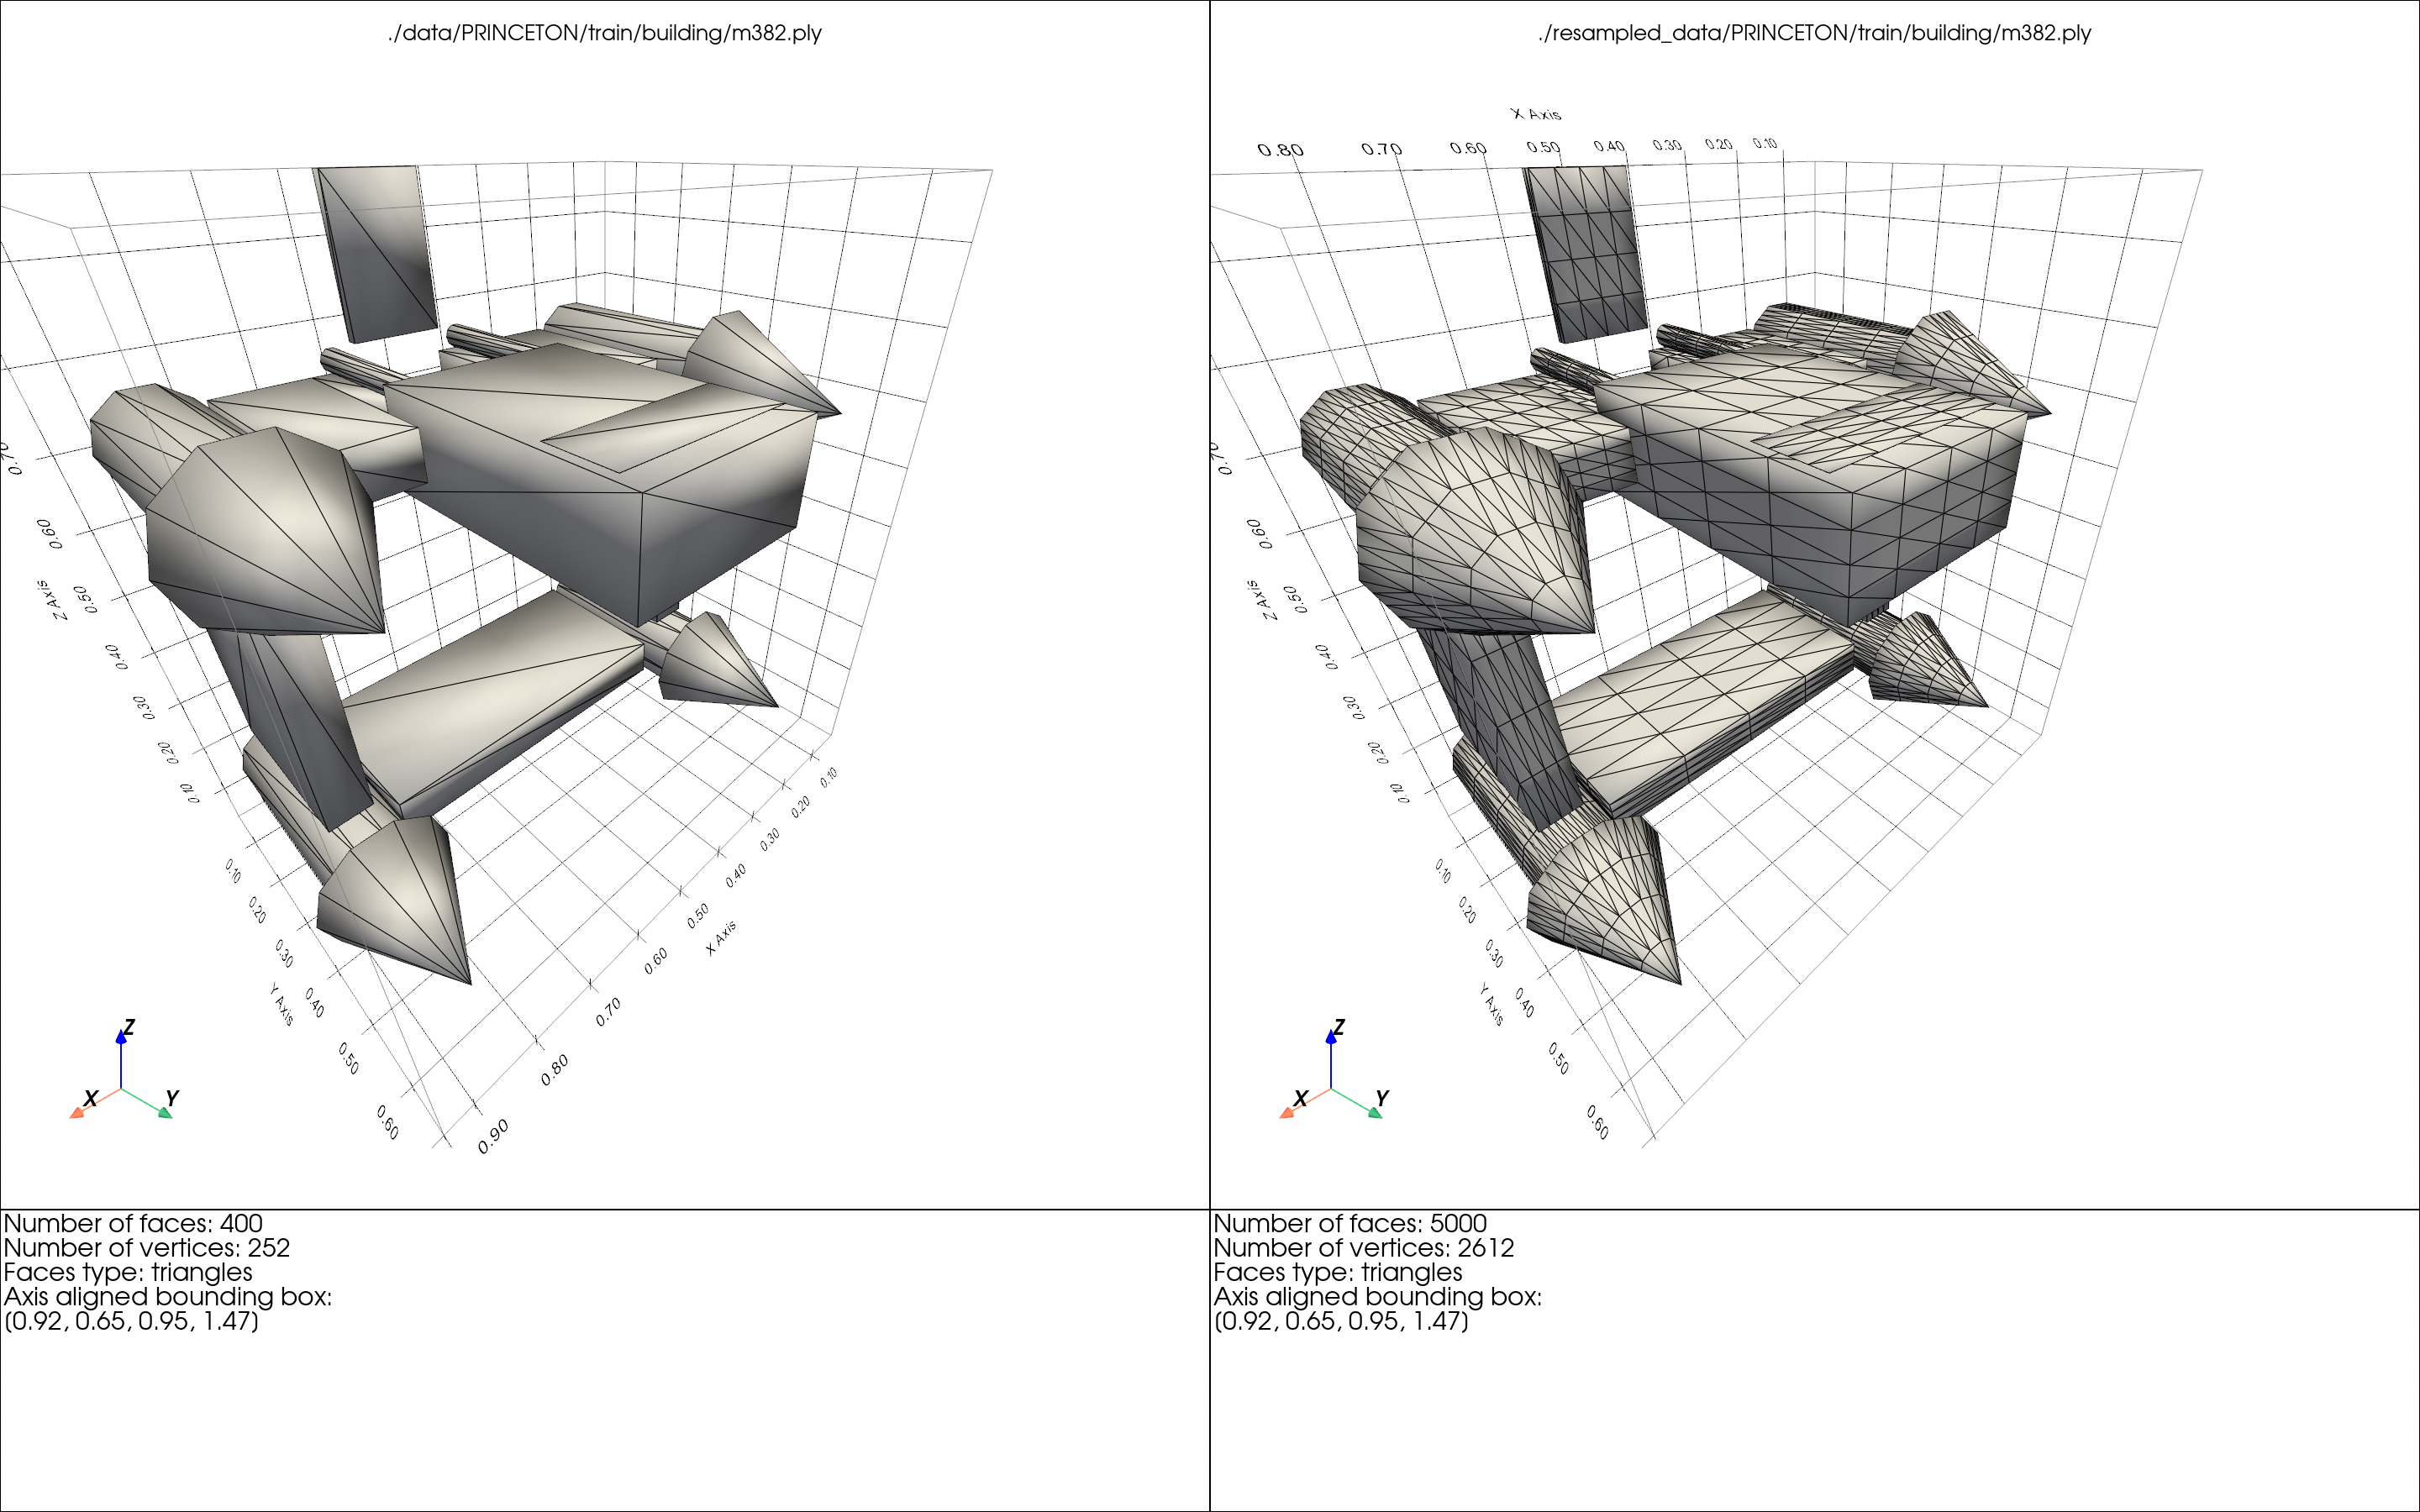
\includegraphics[width=\linewidth]
  {assets/preprocessing/resampling/castle_resampled.png}
  \caption{Comparison of the original 3D mesh of a castle on the left with its resulting super-sampled mesh on the right.}
  \label{fig:resampled_castle}
\end{figure}

\subsection{Normalizing Shapes}
Besides the remeshing of all 3D meshes, we also have to normalize the shapes.
This is very important because the some of the features we extract will be skewed, giving inconsistent results, if the
shapes are not normalized.
The normalization process consists of four steps, each of which is described in detail:
\begin{enumerate}
    \item Translating barycenter to the origin of the centre of the coordinate system
    \item Aligning the shape such as the major eigenvector corresponds to the $x$ axis, the medium corresponds to the $y$ axis and the minor to $z$ axis
    \item Flipping the shape such that the number of vertices at the positive side of each axis is greater than on the negative side
    \item Rescaling the shape to the unit cube
\end{enumerate}

We describe our shapes as meshes.
This is, a shape $\mathcal{S} = (V_{\mathcal{S}}, F_{\mathcal{S}})$, where $V_{\mathcal{S}} \in \mathbb{M}_{N,3}(\mathbb{R})$ and $F_{\mathcal{S}} \in \mathbb{M}_{M,3}(\mathbb{N})$.
We will describe each of these steps as a function of the vertices of a shape: $f_{TR},f_{AL},f_{FL},f_{RS}: \mathbb{M}_{N,3}(\mathbb{R}) \times \mathbb{M}_{M,3}(\mathbb{N}) \rightarrow \mathbb{M}_{N,3}(\mathbb{R}) \times \mathbb{M}_{M,3}(\mathbb{N})$.
The normalisation process then becomes a simple composition of these functions:
\begin{equation}
    \mathcal{S}_{norm} = f_{RS}(f_{FL}(f_{AL}(f_{TR} (\mathcal{S})))) 
\end{equation}

\subsubsection{Translation of the barycenter to the origin}
The shape is described by the vertices 3D coordinates $V_{\mathcal{S}} = 
\begin{pmatrix}
    v_{1,x} & v_{1,y} & v_{1,z} \\
    \vdots & \vdots & \vdots \\
    v_{N,x} & v_{N,y} & v_{N,z} \\
\end{pmatrix}$
The translation to the barycenter is done as follows:
\begin{enumerate}
    \item Compute the barycenter \ref{barycenter_not} of the shape by averaging all vertex locations weighted by their triangle surfaces.
    \item Apply the translation matrix $Tr =
        \begin{pmatrix}
        -b_{\mathcal{S},x} & 0 & 0 \\
        0 & -b_{\mathcal{S},y} & 0 \\
        0 & 0 & -b_{\mathcal{S},z} \\
        \end{pmatrix}$
to the matrix of vertices such that:
\begin{equation}
    f_{TR}(V_{\mathcal{S}}, \cdot) = ((Tr \cdot V_{\mathcal{S}}^T)^T, \cdot)
\end{equation}
This subtracts the barycenter coordinates from all vertices such that the whole shape is translated to a coordinate
system with the barycenter at its origin.
\end{enumerate}


\subsubsection{Aligning the shape eigenvectors to the axes of coordinates}
In order to align the shape along its principal axes (i.e.\ its eigenvectors), we first need to determine the
eigenvectors by performing a principal component analysis.
That is solving the equations:
\begin{equation}
    det(Cov(V_{\mathcal{S}}) - \lambda \cdot \mathbb{I}_N) = 0
\end{equation}
\begin{equation}
    Cov(V_{\mathcal{S}}) \cdot \overrightarrow{v_{\lambda}} = \lambda \cdot \overrightarrow{v_{\lambda}}
\end{equation}

This results in a set of 3 eigenvectors ($\overrightarrow{v_{\lambda_1}}, \overrightarrow{v_{\lambda_2}}, \overrightarrow{v_{\lambda_3}}$).
Observe that the covariance matrix is symmetric, thus, not only do the eigenvectors form a basis in the 3D space, but they are orthogonal to each other.
Therefore, we can simply align the coordinate axes to the eigenvectors by simply applying a rotation matrix to the set of vertices of the shape of interest.
We want all our shapes to be aligned such that the biggest spread is in the direction of the $x$ axis, the medium
spread in the direction of the $y$ axis, and the smallest in the direction of the $z$ axis.
Therefore, prior to constructing the rotation matrix, we do a rearrangement of the eigenvectors such that $\lambda_1 \geq \lambda_2 \geq \lambda_3$.
With this rearrangement, we can define the procedure of aligning to the coordinate axes as follows:
\begin{equation}
    f_{AL}(V_{\mathcal{S}}, \cdot) = ((Ro \cdot V_{\mathcal{S}}^T)^T, \cdot)    
\end{equation}
, where $Ro = \begin{pmatrix}
        v_{\lambda_1,x} & v_{\lambda_1,y} & v_{\lambda_1,z} \\
        v_{\lambda_2,x} & v_{\lambda_2,y} & v_{\lambda_2,z} \\
        v_{\lambda_3,x} & v_{\lambda_3,y} & v_{\lambda_3,z} \\
        \end{pmatrix}$ 
is the rotation matrix that we use for the alignment. 

\subsubsection{Flipping the shape on momentum}
We want to flip the shape with respect to the planes defined by $x=0$, $y=0$ and $z = 0$ such that the shape is more
concentrated in the subspaces $x > 0$, $y > 0$ and $z > 0$ than in the subspaces $x < 0$, $y < 0$ and $z < 0$ respectively.
For simplicity, suppose that we want the shape only to be more concentrated (i.e.\ have more mass) in the subspace $x>0$ than in $x < 0$.
A simple idea is to consider the number of vertices appertaining to each subspace and flip the shape w.r.t.\ the plane $x=0$ if there are more vertices in $x < 0$.
However, this approach would not be ideal.

Consider a case where we have a lot of small triangles faces in $x < 0$, and a few very big triangles in $x > 0$.
Obviously, we would like to flip the shape such that the mass is more in $x > 0 $, which is not the case if we would
only consider the vertex count in each subspace.

A better approach is to consider the centres of the triangles described by vertices instead and their coordinates.
This idea is incorporated in the descriptor $f_i$ (see Table \ref{tab:notations}).
We compute such a descriptor for each plane of interest, namely $f_x, f_y, f_z$.
Using the sign of these descriptors, we can determine whether the shape has to be flipped w.r.t.\ a
certain plane.
This is incorporated in the following formula:
\begin{equation}
    f_{FL}(V_{\mathcal{S}}, \cdot) = ((Fl \cdot V_{\mathcal{S}}^T)^T, \cdot)
\end{equation},
where $Fl = \begin{pmatrix}
    sign(f_x) & 0 & 0 \\
    0 & sign(f_y) & 0 \\
    0 & 0 & sign(f_z) \\
\end{pmatrix}$ is the flipping decision matrix.

\subsubsection{Rescale shape to unit cube}
Since 3D models can be rescaled, in our application, we do not care about the size of the shapes in our database.
So that this does not cause issues for us when we compute features, we want to standardize the size of all shapes.
We chose to rescale them relative to their unit cube.
To achieve this, we simply multiply each vertex by a rescaling factor \ref{rescale_not}.

\begin{equation}
    f_{RS}(V_{\mathcal{S}}, \cdot) = (\sigma_{unit}(S) \cdot V_{\mathcal{S}}, \cdot)
\end{equation}

\subsection{Preprocessing results}

\subsubsection{Resampling}
In order to test how well our resampling pipeline worked, we compute the distribution histograms of the number of
faces and vertices before and after processing our processing.

The results are shown in Figure \ref{fig:resampling-faces-vertices}.
After resampling, nearly all shapes have exactly $5000$ faces and $2500$ vertices.

\begin{figure}[H]
    \centering
    \begin{subfigure}[b]{0.45\textwidth}
        \centering
        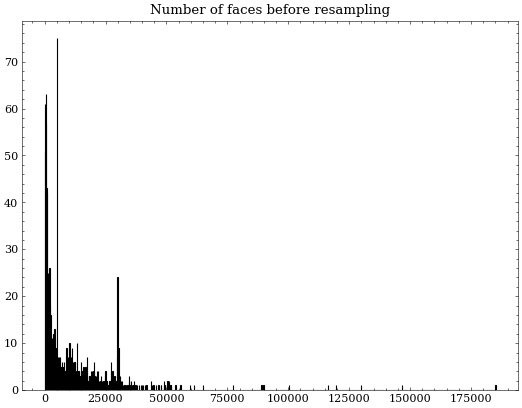
\includegraphics[width=\textwidth]{assets/preprocessing/Number_of_faces_before_resampling.png}
        \caption{Faces before resampling}
        \label{fig:resampling-faces-before}
    \end{subfigure}
    \hfill
    \begin{subfigure}[b]{0.45\textwidth}
        \centering
        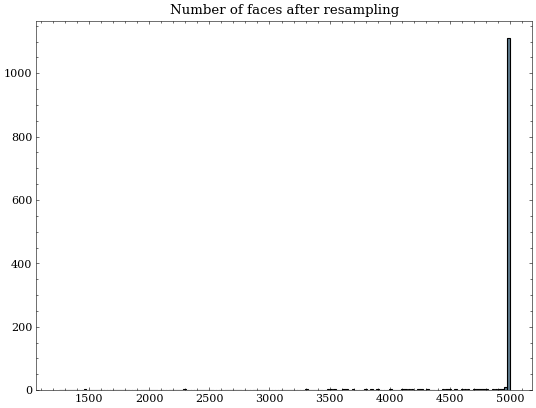
\includegraphics[width=\textwidth]{assets/preprocessing/Number_of_faces_after_resampling.png}
        \caption{Faces after resampling}
        \label{fig:resampling-faces-after}
    \end{subfigure}

\vspace{1cm}
    \begin{subfigure}[b]{0.45\textwidth}
        \centering
        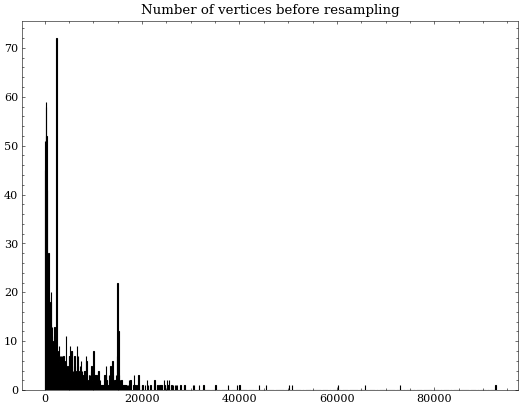
\includegraphics[width=\textwidth]{assets/preprocessing/Number_of_vertices_before_resampling.png}
        \caption{Vertices before resampling}
        \label{fig:resampling-vertices-before}
    \end{subfigure}
    \hfill
    \begin{subfigure}[b]{0.45\textwidth}
        \centering
        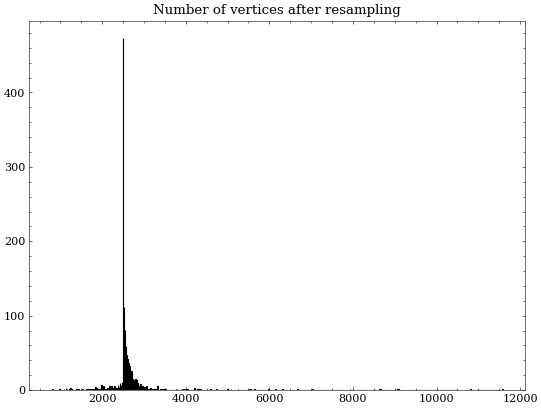
\includegraphics[width=\textwidth]{assets/preprocessing/Number_of_vertices_after_resampling.png}
        \caption{Vertices after resampling}
        \label{fig:resampling-vertices-after}
    \end{subfigure}
    \caption{Distribution of the number the number of faces \& vertices}
    \label{fig:resampling-faces-vertices}
\end{figure}

\subsubsection{Normalisation}
For testing the results of the normalisation, we compute histograms before and after, which we use to check some
pre-defined requirements regarding each step.

\paragraph{Centering}
In order to check that the barycenter of the shape is in the origin of the coordinate system, we compute the distance from the barycenter to the origin: $d(b_{\mathcal{S}}, (0,0,0))$.
For the processed - centered, shapes, we would expect the distance to be $0$.
We then plot a histogram to show the distribution of these distances, shown in Figure \ref{fig:resampling-barycenter}.

Before the normalisation, a small number of shapes have the barycenter far away from the origin (i.e.\ $d
($\ref{barycenter_not}$, (0,0,0)) \approx 3^{21}$.
After the normalisation, the biggest distance is approximately $0.002$.

The fact that we have a couple of shapes that deviate from our ideal distance is because of floating-point
approximations when computing the barycenter.
All in all, the results for this normalisation step are satisfying.

\begin{figure}[H]
    \centering
    \begin{subfigure}[b]{0.45\textwidth}
        \centering
        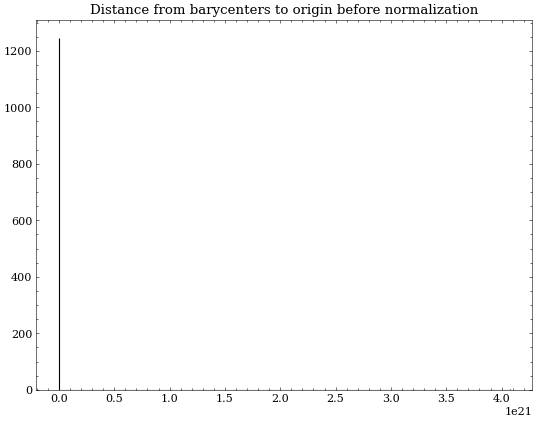
\includegraphics[width=\textwidth]{assets/preprocessing/Distance_from_barycenters_to_origin_before_normalization.png}
        \caption{Distance before normalisation}
        \label{fig:resampling-barycenter-before}
    \end{subfigure}
    \hfill
    \begin{subfigure}[b]{0.45\textwidth}
        \centering
        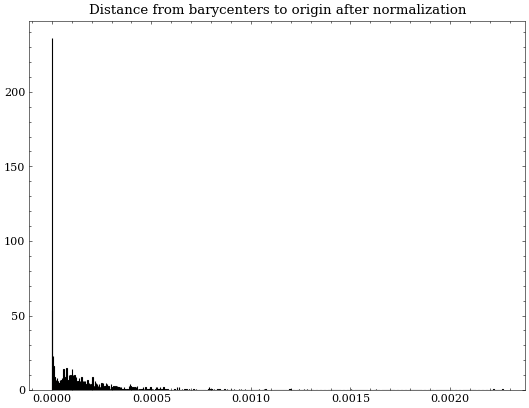
\includegraphics[width=\textwidth]{assets/preprocessing/Distance_from_barycenters_to_origin_after_normalization.png}
        \caption{Distance after normalisation}
        \label{fig:resampling-barycenter-after}
    \end{subfigure}
    \caption{Distribution of the distance from the barycenter to the origin}
    \label{fig:resampling-barycenter}
\end{figure}

\paragraph{Alignment}
After aligning to the principal component axes (i.e.\ eigenvectors), we expect the shape eigenvectors to be exactly equal to the coordinate axis vectors.

To test this, for each axis, we compute the distribution of the dot product of the corresponding eigenvector to that axis.
For instance, for the $x$-axis, we compute $ \overrightarrow{x} \cdot \overrightarrow{v_{\lambda_1}}$ where $\overrightarrow{x} = (1, 0, 0)$ and $\overrightarrow{v_{\lambda_1}}$ is the vector indicating the direction in which the shape have the maximal spread of the vertices.
The histograms from before and after this step can be seen in Figure \ref{fig:resampling-alignment}.
If the shapes are aligned correctly, this dot product should be equal to 1, since the angle should be 0.
This is what we observe in our histograms.

\begin{figure}[H]
    \centering
    \begin{subfigure}[b]{0.45\textwidth}
        \centering
        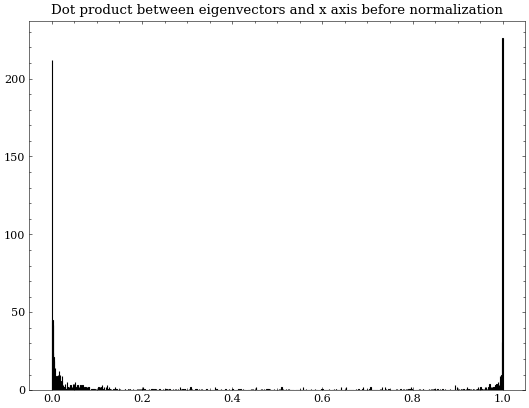
\includegraphics[width=\textwidth]{assets/preprocessing/Dot_product_between_eigenvectors_and_x_axis_before_normalization.png}
        \caption{Major eigenvector \& $x$ axis before normalisation}
        \label{fig:resampling-alignment-x-before}
    \end{subfigure}
    \hfill
    \begin{subfigure}[b]{0.45\textwidth}
        \centering
        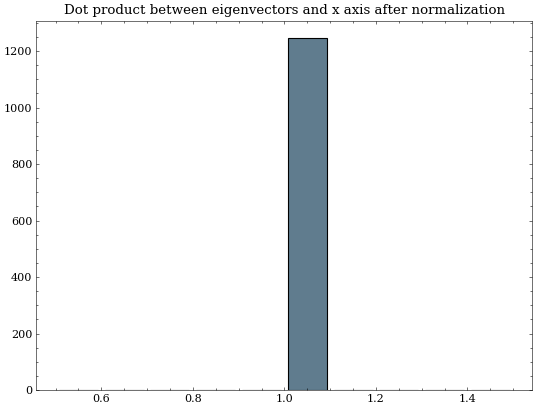
\includegraphics[width=\textwidth]{assets/preprocessing/Dot_product_between_eigenvectors_and_x_axis_after_normalization.png}
        \caption{Major eigenvector\& $x$ axis after normalisation}
        \label{fig:resampling-alignment-x-after}
    \end{subfigure}
    
\vspace{1cm}
    \begin{subfigure}[b]{0.45\textwidth}
        \centering
        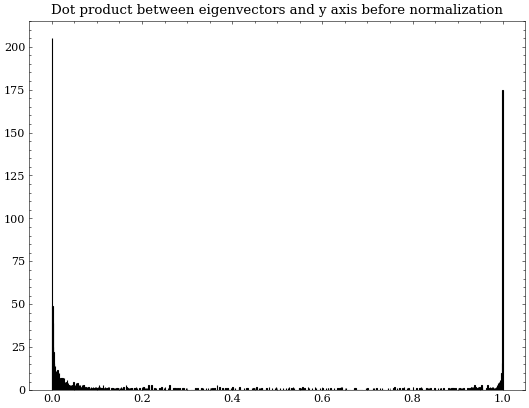
\includegraphics[width=\textwidth]{assets/preprocessing/Dot_product_between_eigenvectors_and_y_axis_before_normalization.png}
        \caption{Medium eigenvector \& $y$ axis before normalisation}
        \label{fig:resampling-alignment-y-before}
    \end{subfigure}
    \hfill
    \begin{subfigure}[b]{0.45\textwidth}
        \centering
        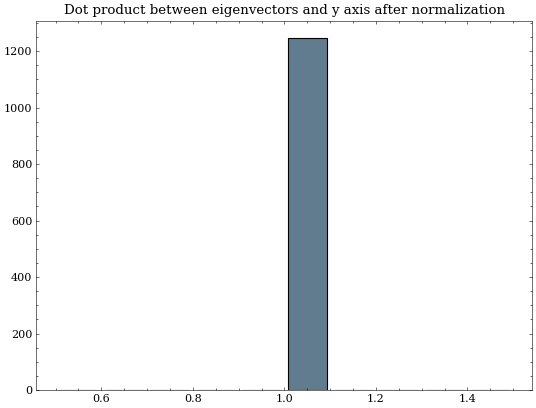
\includegraphics[width=\textwidth]{assets/preprocessing/Dot_product_between_eigenvectors_and_y_axis_after_normalization.png}
        \caption{Medium eigenvector \& $y$ axis after normalisation}
        \label{fig:resampling-alignment-y-after}
    \end{subfigure}

\vspace{1cm}
    \begin{subfigure}[b]{0.45\textwidth}
        \centering
        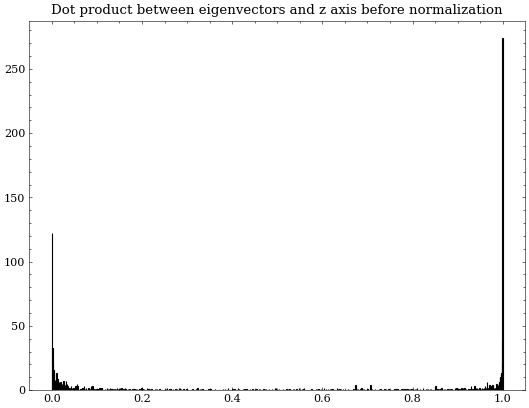
\includegraphics[width=\textwidth]{assets/preprocessing/Dot_product_between_eigenvectors_and_z_axis_before_normalization.png}
        \caption{Minor eigenvector \& $z$ axis before normalisation}
        \label{fig:resampling-alignment-z-before}
    \end{subfigure}
    \hfill
    \begin{subfigure}[b]{0.45\textwidth}
        \centering
        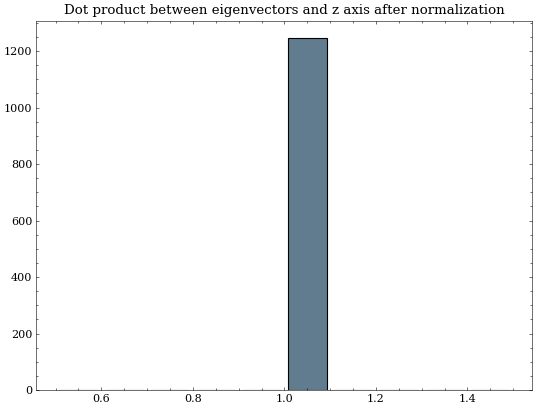
\includegraphics[width=\textwidth]{assets/preprocessing/Dot_product_between_eigenvectors_and_z_axis_after_normalization.png}
        \caption{Minor eigenvector \& $z$ axis after normalisation}
        \label{fig:resampling-alignment-z-after}
    \end{subfigure}
    \caption{Distribution of the dot product between an eigenvector and its respective coordinate axis}
    \label{fig:resampling-alignment}
\end{figure}


\paragraph{Flipping}
In a correctly implemented flipping step, we would expect the shape to have more mass on the positive side of
each plane $x = 0, y = 0, z = 0$.
We check whether this is the case by computing the flipping momentum components (i.e.\ \ref{flip_axis_not}) and
testing if they are positive.
If they are, then we flipped the shape correctly.

We calculate the weighted difference in the number of vertices on the positive and negative sides of $x = 0, y = 0, z
= 0$.
We plot the distributions before and after normalisation, shown in Figure \ref{fig:resampling-flipping}.
The histograms show that, after normalisation, we do have a positive difference - meaning, the flipping process is working as intended.

\begin{figure}[H]
    \centering
    \begin{subfigure}[b]{0.45\textwidth}
        \centering
        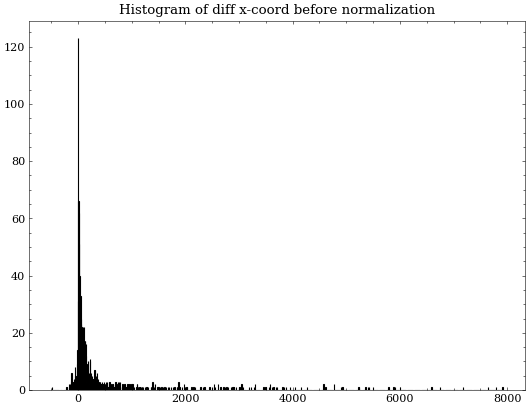
\includegraphics[width=\textwidth]{assets/preprocessing/Histogram_of_diff_x-coord_before_normalization.png}
        \caption{$x=0$ plane before normalisation}
        \label{fig:resampling-flipping-x-before}
    \end{subfigure}
    \hfill
    \begin{subfigure}[b]{0.45\textwidth}
        \centering
        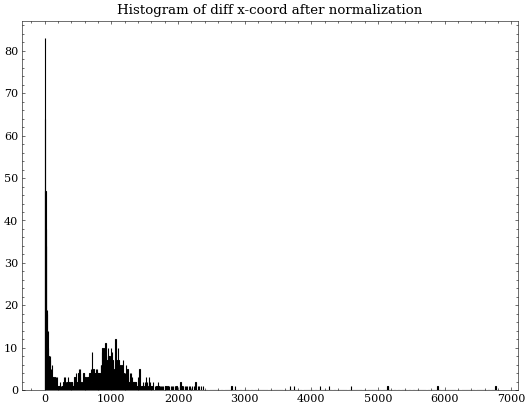
\includegraphics[width=\textwidth]{assets/preprocessing/Histogram_of_diff_x-coord_after_normalization.png}
        \caption{$x=0$ plane after normalisation}
        \label{fig:resampling-flipping-x-after}
    \end{subfigure}
    
\vspace{1cm}
    \begin{subfigure}[b]{0.45\textwidth}
        \centering
        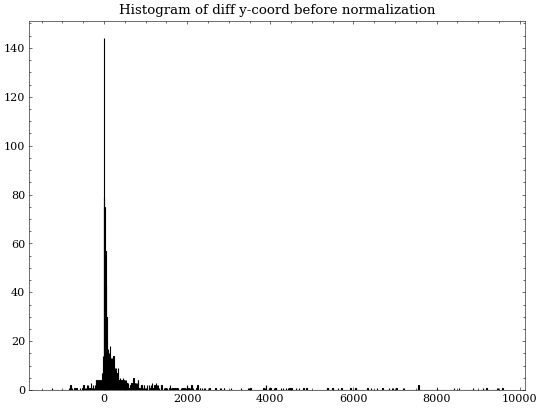
\includegraphics[width=\textwidth]{assets/preprocessing/Histogram_of_diff_y-coord_before_normalization.png}
        \caption{$y=0$ plane before normalisation}
        \label{fig:resampling-flipping-y-before}
    \end{subfigure}
    \hfill
    \begin{subfigure}[b]{0.45\textwidth}
        \centering
        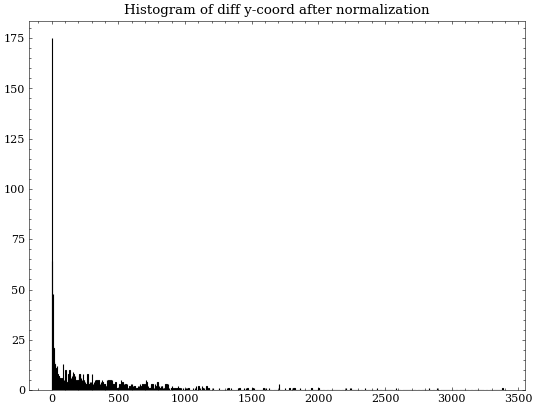
\includegraphics[width=\textwidth]{assets/preprocessing/Histogram_of_diff_y-coord_after_normalization.png}
        \caption{$y=0$ plane after normalisation}
        \label{fig:resampling-flipping-y-after}
    \end{subfigure}

\vspace{1cm}
    \begin{subfigure}[b]{0.45\textwidth}
        \centering
        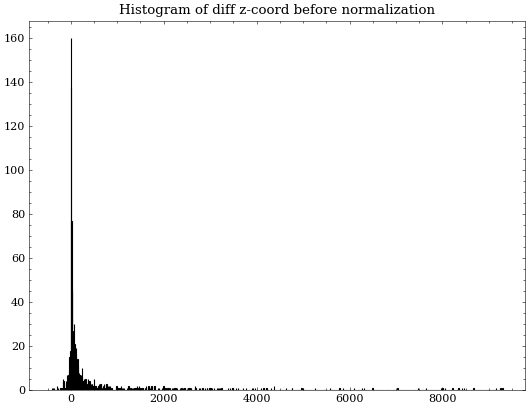
\includegraphics[width=\textwidth]{assets/preprocessing/Histogram_of_diff_z-coord_before_normalization.png}
        \caption{$z=0$ plane before normalisation}
        \label{fig:resampling-flipping-z-before}
    \end{subfigure}
    \hfill
    \begin{subfigure}[b]{0.45\textwidth}
        \centering
        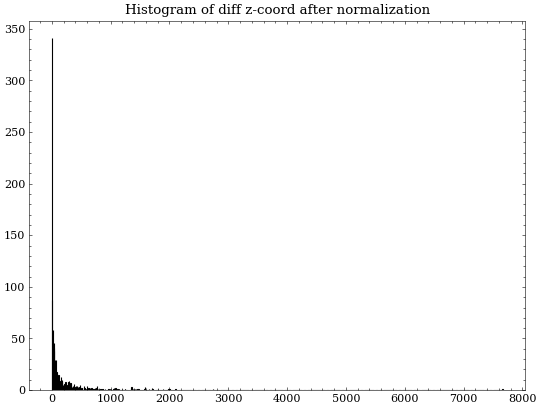
\includegraphics[width=\textwidth]{assets/preprocessing/Histogram_of_diff_z-coord_after_normalization.png}
        \caption{$z=0$ plane after normalisation}
        \label{fig:resampling-flipping-z-after}
    \end{subfigure}
    \caption{Distribution of the weighted difference of the number of vertices on the positive and negative sides of all axis planes}
    \label{fig:resampling-flipping}
\end{figure}


\paragraph{Scaling}
To check whether the shapes are rescaled correctly, we analyse the bounding box diagonal of the shape.
For a shape contained in the unit cube, the bounding box diagonal cannot be greater than $\sqrt{3} \approx 1.732$.

We plot the distribution of the diagonals before and after normalisation, shown in Figure \ref{fig:resampling-diagonal}.
After normalisation, all lengths are between $1$ and $1.73$, which is what we would expect for correctly rescaled shapes.

\begin{figure}[ht]
    \centering
    \begin{subfigure}[b]{0.45\textwidth}
        \centering
        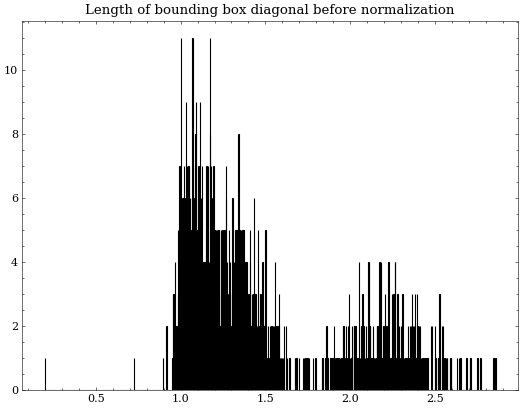
\includegraphics[width=\textwidth]{assets/preprocessing/Length_of_bounding_box_diagonal_before_normalization.png}
        \caption{Length before normalisation}
        \label{fig:resampling-diagonal-before}
    \end{subfigure}
    \hfill
    \begin{subfigure}[b]{0.45\textwidth}
        \centering
        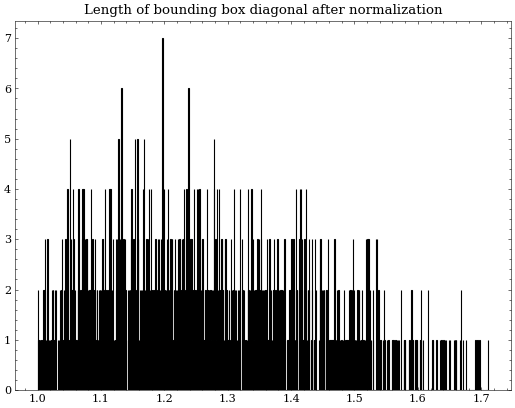
\includegraphics[width=\textwidth]{assets/preprocessing/Length_of_bounding_box_diagonal_after_normalization.png}
        \caption{Length after normalisation}
        \label{fig:resampling-diagonal-after}
    \end{subfigure}
    \caption{Distribution of the lengths of the bounding box diagonals}
    \label{fig:resampling-diagonal}
\end{figure}

\begin{figure}[ht]
    \centering
    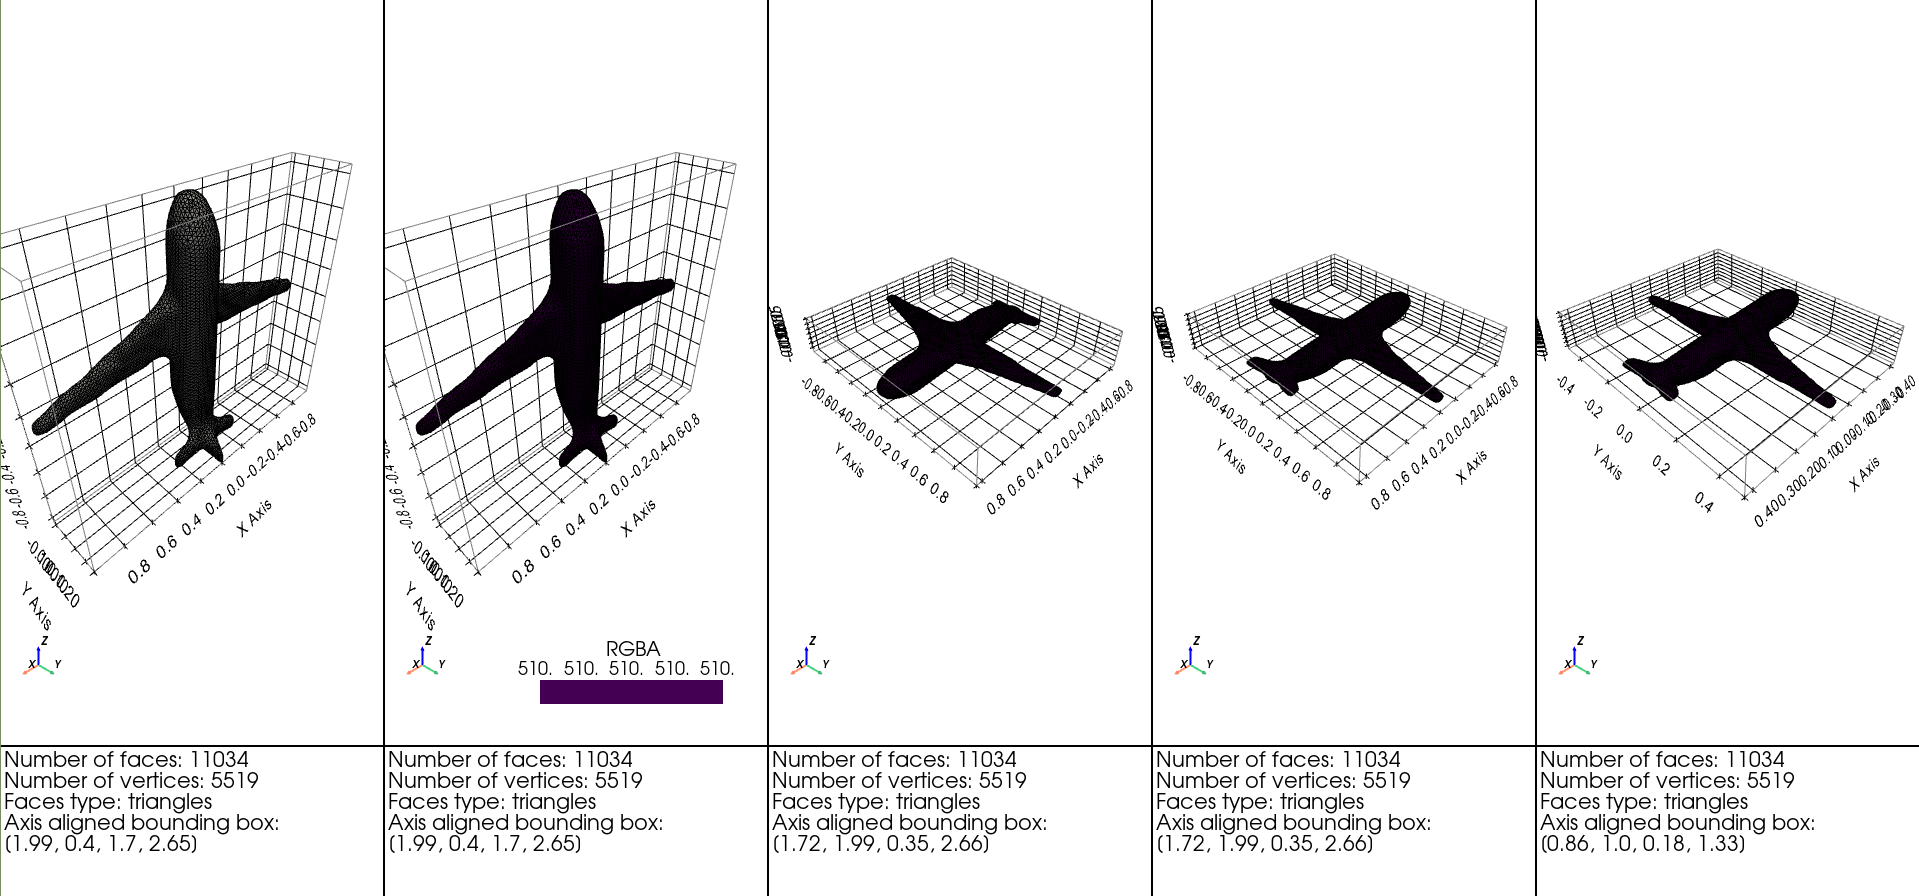
\includegraphics[width = 0.9\textwidth]{assets/visualisation/normalization_process.png}
    \caption{Normalisation process by steps}
    \label{fig:normalization-by-steps}
\end{figure}

Figure \ref{fig:normalization-by-steps} presents the step-by-step process of an airplane model going through
the normalization process.

\section{Feature extraction}
\label{section:feature-extraction}
In order to discriminate the shapes in our database, we describe each shape by a set of features.
We then use these features to compute a distance between a pair of shapes, which is relative to how dissimilar the two
shapes are.
This section discusses exactly what features we determine for each shape, how we calculate them, and how we
implemented these calculations.
An overview of all features that will be extracted for the 3D shapes can be seen in Table \ref{tab:features}.

\paragraph{Global descriptors}
Firstly, we compute some elementary descriptors for 3D objects, which are single values describing a shape from a
global perspective.
These features are the surface area, volume, diameter, eccentricity, and compactness of the shape, as well as three
ratios for comparisons between the shape and its bounding box or convex hull.

The bounding box of a 3D shape is the smallest rectangular box which fully encompasses the volume of the 3D shape.
We use the ratio between the volume of the shape  the volume of its bounding box, to moderately indicate how tightly
the shape fits in a rectangular box.

The convex hull of a 3D shape is the convex shape with the smallest volume that fully encompasses the shape.
Another way to think of the convex hull is the shape with the smallest total surface area which encompasses the 3D shape.
We determine the ratio between the volume of the shape and the volume of its convex hull, as well as the
ratio of the surface area to the surface area of its convex hull.
These two ratios give an indication of how convex the shape is.

\paragraph{Local descriptors}
The local descriptors we use are the so-called $A3$, $D1$, $D2$, $D3$ and $D4$ descriptors.
The descriptors follow a naming convention, measuring either an angle, $A$, or a distance, $D$, and considering a
certain number of vertices, either $1$, $2$, $3$ or $4$.
The $A3$ descriptor measures the angle between three vertices, $D1$ measures the distance of a vertex to the barycenter of the shape, $D2$ measures the distance between two vertices, $D3$ measures the area of the surface constructed from three vertices and $D4$ measures the volume of the tetrahedron formed by four vertices.
The $D3$ and $D4$ descriptors are not directly measuring distances, but in order to give equal power to the distance descriptors, these two descriptors are scaled to the same unit of measurement, a distance.

We are using the local descriptors $A3$, $D1$, $D2$, $D3$ and $D4$, because they are easy to compute and generally have
the same distribution of values for similar shapes - shapes of the same classes.
Although the computations are easy to do for one configuration of vertices, we have to perform the calculations many times, since the values describe the shape at a local level.

Looking at only one such descriptor might not be sufficient for distinguishing different shapes, but collectively they are very powerful in recognizing similar shapes.
Each one of the five local descriptors gives information about a narrow part of a shape, but what we would like to
have is an intuition about how these local features change from one shape to another.
Thus, we would like to capture the feature with respect to a shape over all its regions, rather than only a snapshot
of a region of the shape.
In order to do this, we compute the distribution of the values of the descriptor given the shape.
For most descriptors, calculating the distribution exhaustively is unfeasible, since the entire search space for the
combinations of local areas can grow very large.
Consequently, for all of these descriptors, we compute an approximation of the distribution by considering several
samples from the shape and computing the histogram of the descriptor values given these samples.
We would like to use these histograms (i.e.\ approximations of distributions) as feature vectors .

However, just considering the values and their frequencies would not work, because this will make the feature vector
large and have a variable size.
To mitigate this, we aggregate these values to get a fixed-size relative small feature vector for each such descriptor.
For this approach we need to know beforehand the range in which the values for such a descriptor are.
Luckily, due to the fact that our shapes are re-scaled to the unit cube in the preprocessing step, we can compute
such ranges.
The exact values can be found in Table \ref{tab:feature-histogram-ranges}.
We typically aggregate these values such that we end up with a histogram with $20-30$ bins, the exact dimension for each feature vector as well as the number of samples considered to compute them are specified in Table \ref{tab:features}.

\begin{table}[ht]
    \centering
    \resizebox{\textwidth}{!}{
    \begin{tabular}{c|c|c}
        \textbf{Feature name} & \textbf{Notation} & \textbf{Description/Formula}  \\
        \hline
        Surface area & $A_{\mathcal{S}}$ & $A_{\mathcal{S}} = \sum_{\mathcal{T} \in F} A_{\mathcal{T}}$ \\
        \hline
        Volume & $Vol_{\mathcal{S}}$ & $Vol_{\mathcal{S}} = | \sum\limits_{\mathcal{T}h_O = \mathcal{T},\mathcal{T} \in F} Vol_{\mathcal{T}h_O} |$ \\
        \hline
        Diameter & $d_{\mathcal{S}}$ & $d_{\mathcal{S}} = max_{v_1, v_2 \in V_{\mathcal{S}}} || (v_2 - v_1) ||$ \\
        \hline
        Eccentricity & $ecc_{\mathcal{S}}$ & $ecc_{\mathcal{S}} = |\lambda_{\mathcal{S}, 1}| / |\lambda_{\mathcal{S}, 3}|$ \\
        \hline
        Compactness & $compactness_{\mathcal{S}}$ & $compactness_{\mathcal{S}} = A_{\mathcal{S}}^3 / (36\pi \cdot Vol_{\mathcal{S}}^2)$ \\
        \hline
        Ratio volume to bounding box volume & $Vol_{\mathcal{S}} / Vol_{\mathcal{S}}^{bbox}$ & An indicator of how close is the shape volume to its bounding box volume\\
        \hline
        Ratio volume to convex hull volume & $Vol_{\mathcal{S}} / Vol_{\mathcal{S}}^{CH}$ & An indicator of how close if the shape volume to the volume of the convex hull of the shape\\
        \hline
        Ratio area to convex hull area & $A_{\mathcal{S}} / A_{\mathcal{S}}^{CH}$ & An indicator of how close if the shape surface to the surface of the convex hull of the shape\\
        \hline
        
        & & Normalized histogram of the distribution of the angles between  \\
        Angle distribution & $A3$ & 3 random vertices of the shape (Figure \ref{fig:local_descriptor_visualisation_A3}) \\
        & & as an \textbf{26}-dimensional vector (\textbf{700} samples of vertices triplets)\\
        \hline

        & & Normalized histogram of the distribution of the distance between  \\
        Distance distribution 1 & $D1$ & a random vertex of the shape and the origin (Figure \ref{fig:local_descriptor_visualisation_D1})\\
        & & as a \textbf{21}-dimensional vector (\textbf{1500} samples of vertices)\\
        \hline
        
        & & Normalized histogram of the distribution of the distance between  \\
        Distance distribution 2 & $D2$ & two random vertices of the shape (Figure \ref{fig:local_descriptor_visualisation_D2})\\
        & & as a \textbf{23}-dimensional vector (\textbf{1000} samples of vertices pairs)\\
        \hline
        
        & & Normalized histogram of the distribution of the squared root of triangle area \\
        Distance distribution 3 & $D3$ & formed by 3 random vertices of the shape (Figure \ref{fig:local_descriptor_visualisation_D3})\\
        & & as a \textbf{26}-dimensional vector (\textbf{700} samples of vertices triplets)\\
        \hline
        
        & & Normalized histogram of the distribution of cube root of tetrahedron volume \\
        Distance distribution 4 & $D4$ & formed by 4 random vertices of the shape (Figure \ref{fig:local_descriptor_visualisation_D4})\\
        & & as a \textbf{30}-dimensional vector (\textbf{500} samples of vertices quadruplets)\\
    \end{tabular}
    }
    \caption{Features for a shape $\mathcal{S}$}
    \label{tab:features}
\end{table}

\begin{table}[ht]
    \centering
    \begin{tabular}{c|c}
        Feature & Range \\
        \hline
        A3 & $[0, \pi]$ \\
        D1 & $[0, \sqrt{3}]$\\
        D2 & $[0, \sqrt{3}]$\\
        D3 & $[0, \sqrt{\sqrt{3}/2}]$\\
        D4 & $[0, \sqrt[3]{1/3}]$\\
    \end{tabular}
    \caption{Theoretical lower and upper bounds for features A3,D1,D2,D3,D4}
    \label{tab:feature-histogram-ranges}
\end{table}

\paragraph{Theoretical bounds for local descriptors}
The $A3$ descriptor computes the angle between 3 random vertices.
Since we consider the smaller angle in radians we  know that the values must be in the range $[0, 180^{\circ}]$, or
$[0, \pi]$.

For each of the distance descriptors $D1, D2, D3, D4$, the lower bound for the values is 0 because the distance is
positive.

For $D1$, we compute the distance from the barycenter to a random vertex.
The worst-case scenario is when the barycenter and the vertex coincide with two diametral opposite vertices of the unit cube, meaning the distance between them is the diagonal of the unit cube, which is $\sqrt{3}$.
The same argumentation also holds for $D2$.

For $D3$, we compute the area between 3 random vertices.
The maximum area of a triangle inscribed in the unit cube is $\sqrt{3}/2$.
Since for $D3$ we consider the square root of the area in order to have the same dimensionality as $D1$ and $D2$ the upper bound of the range of the values of $D3$ is $\sqrt{\sqrt{3} /2 }$.

Lastly, for $D4$ we look at four random vertices and compute the volume of the tetrahedron formed by these vertices.
Let us denote the unit cube by $A, B, C, D, A', B', C', D'$.
For example, consider the tetrahedron $A, B, C, B'$ - a tetrahedron with the maximum volume inscribed in the unit cube.
The volume of this tetrahedron is $1/3$.
Here we again want to have the same dimensionality as the other distance descriptors, therefore we need to take the cube root of this value, since we are dealing with a volume.
Thus the theoretical maximum value for the $D4$ descriptor is $\sqrt[3]{1/3}$.

\paragraph{Checking the global descriptors}
In order to check that our computations of the global descriptors are performed correctly, we check using 3 basic
shapes, for which we can easily compute the expected values from the formulas, and compare them to our results.
In Table \ref{tab:proof-global-features} we present the theoretical values of the global descriptors for a Sphere,
a Cylinder and a Torus.
Figures \ref{fig:sphere-scalars}, \ref{fig:cylinder-scalars} and \ref{fig:torus-scalars} present these shapes and the
values our system computed for the global descriptors.

Notice that the computed values are approximately the same as the theoretical ones.
Obviously, the computed values are approximations of the theoretical ones because the shapes from which we compute them represent a sampled signal of the original one.
In other words, the shape from which we compute our descriptors is already an approximation of the theoretical shape from which we compute the theoretical values for the descriptors.
However, the fact that differences between the theoretical values and the computed ones are negligible proves that our implementation for the computation of these descriptors is correct.

\subsection{Results}
\paragraph{Global descriptors}
In Figure \ref{fig:global-descriptors-dataset} we show the global descriptors for some shapes from our dataset.
Comparing the scalar values for these shapes, we see that indeed they tend to describe the shape correctly.

Consider Figures \ref{fig:bridge-scalars} and \ref{fig:cup-scalars}, and notice how the volume and surface area of the
cup is bigger than the volume of the bridge.
On the other hand, notice how the eccentricity of elongated shapes is considerably larger - take again the cup-bridge
example.
Also, notice how the diameter value for the shape presented in Figure \ref{fig:table-scalars} is almost the same as
the bounding box diameter which is what we would expect, because the elements that compose the table
(i.e.\ 4 legs and the table top) are very close to the boundaries of the bounding box.

\paragraph{Local descriptors}
For the local descriptors, we perform an empirical experiment to test the correctness of our implementation.
For each descriptor, we take a sample of 20 shapes from each class in our dataset and display the computed histograms.
Usually, shapes from similar classes would tend to have similar local features.
Thus, the distributions over the shapes of a local feature should be similar if the shapes are similar.

Figures \ref{fig:A3-signatures-1} and \ref{fig:A3-signatures-2} show the result of these experiments per class for the descriptor $A3$.
Notice how for each class the shapes' signatures (i.e.\ histograms) are similar.
This proves empirically that our implementation of $A3$ is correct.
The same argumentation is valid for the other descriptors - $D1$ (see Figures \ref{fig:D1-signatures-1} and
\ref{fig:D1-signatures-2}), $D2$ (see Figures \ref{fig:D2-signatures-1} and \ref{fig:D2-signatures-2}), $D3$ (see
Figures \ref{fig:D3-signatures-1} and \ref{fig:D3-signatures-2}) and $D4$ (see Figures \ref{fig:D4-signatures-1} and \ref{fig:D4-signatures-2}).

\begin{table}[ht]
    \centering
    \begin{tabular}{c|c}
        \textbf{Scalar Feature} & \textbf{Theoretical value} \\
        \hline
        \multicolumn{2}{c}{\textbf{Sphere} $R = 1$} \\
        \hline
        Volume & $\frac{4}{3} \pi R^3 = \frac{4}{3} \pi$ \\
        Surface area & $4 \pi R^2 = 4 \pi$\\
        Compactness & 1\\
        Eccentricity & 1\\
        Bounding box volume & 1\\
        Diameter & $2R = 2$\\
        Convex hull volume & $\frac{4}{3} \pi R^3 = \frac{4}{3} \pi$\\
        Convex hull area & $4 \pi R^2 = 4 \pi$\\
        
        \hline
        \multicolumn{2}{c}{\textbf{Cylinder} $r = 1, h = 5$} \\
        \hline
        Volume & $\pi \cdot r^2 \cdot h = 5 \pi$ \\
        Surface area & $2 \pi \cdot r^2 + 2 \pi \cdot r \cdot h = 2\pi + 10\pi = 12\pi$\\
        Compactness & $Area_{cylinder}^3 / (36\pi \cdot Vol_{cylinder}^2) = (12\pi)^3 / (36\pi \cdot 5\pi) = 9.6\pi$\\
        Eccentricity & -\\
        Bounding box volume & $2 \cdot 2 \cdot 5 = 20$\\
        Diameter & $\sqrt{(2r)^2 + h^2} = \sqrt{29}$\\
        Convex hull volume & $5\pi$\\
        Convex hull area & $12\pi$\\

        \hline
        \multicolumn{2}{c}{\textbf{Torus} $r = 1/2, R = 1$} \\
        \hline
        Volume & $2 \pi^2 \cdot R \cdot r^2 = \frac{\pi^2}{2}$ \\
        Surface area & $4 \pi^2 \cdot R \cdot r = 2 \pi^2$\\
        Compactness & $Area_{torus}^3 / (36\pi \cdot Vol_{torus}^2) = 8\pi^6 / (9\pi^5) = \frac{8}{9}\pi$\\
        Eccentricity & -\\
        Bounding box volume & $3 \cdot 3 \cdot 1 = 9$\\
        Diameter & $R + 2r = 3$\\
        Convex hull volume & $2\pi \cdot R \cdot 2r + \frac{4}{3}\pi r^3=  2\pi + \frac{\pi}{6}$\\
        Convex hull area & $2\cdot 2\pi R + 2\pi \cdot \pi r = 4\pi + \pi^2$\\
        
    \end{tabular}
    \caption{Feature theoretical values for several shapes}
    \label{tab:proof-global-features}
\end{table}

\begin{figure}[ht!p]
    \centering
    \begin{subfigure}[b]{0.45\textwidth}
        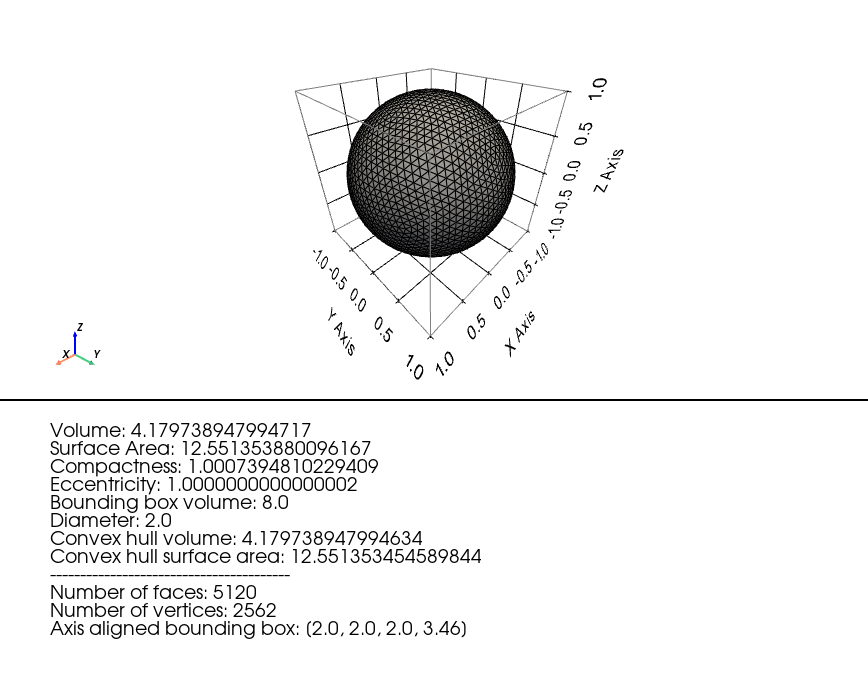
\includegraphics[width=\textwidth]{assets/feature_extraction/scalar_features/sphere.png}
    \caption{Sphere scalar features}
    \label{fig:sphere-scalars}    
    \end{subfigure}
    \hfill
    \begin{subfigure}[b]{0.45\textwidth}
        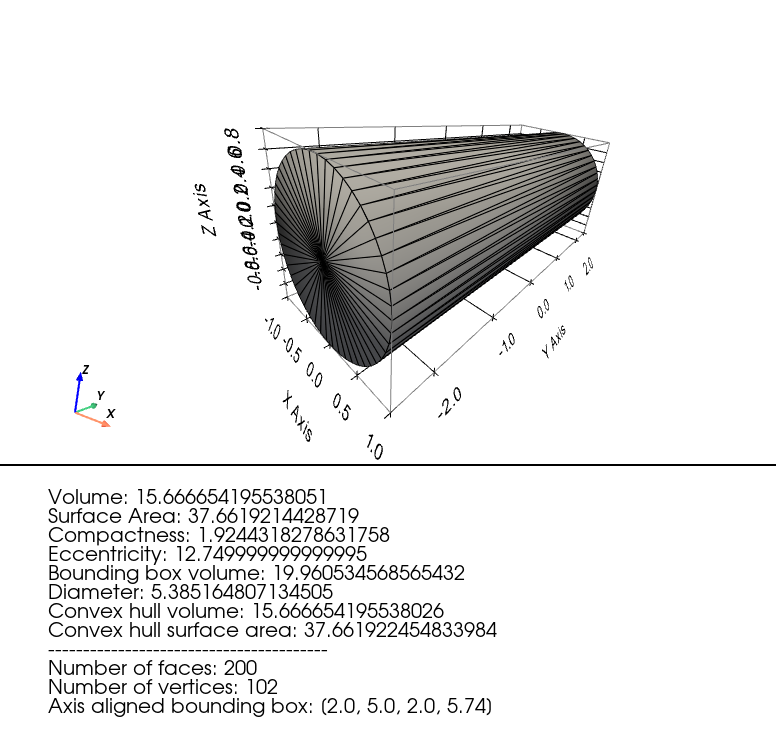
\includegraphics[width=\textwidth]{assets/feature_extraction/scalar_features/cylinder.png}
    \caption{Cylinder scalar features}
    \label{fig:cylinder-scalars}
    \end{subfigure}
    \hfill
    
    \begin{subfigure}[b]{0.45\textwidth}
        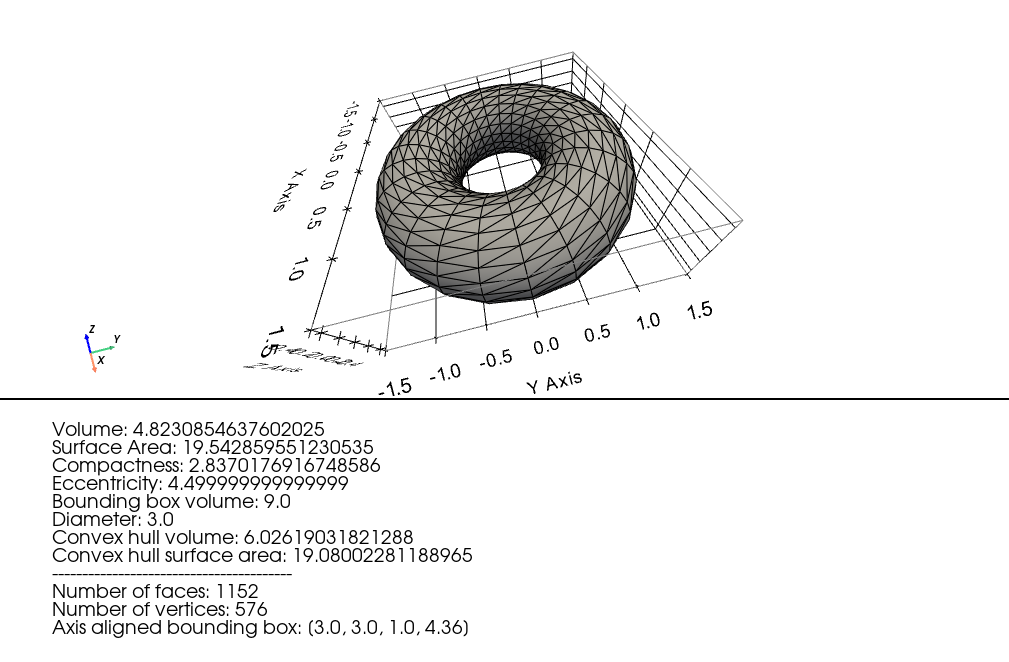
\includegraphics[width=\textwidth]{assets/feature_extraction/scalar_features/torus.png}
    \caption{Torus scalar features}
    \label{fig:torus-scalars}   
    \end{subfigure}

    \caption{Global descriptors for several 3D shapes}
    \label{fig:global-descriptors-proof} 
\end{figure}


\begin{figure}[ht!p]
    \centering
    \begin{subfigure}[b]{0.45\textwidth}
        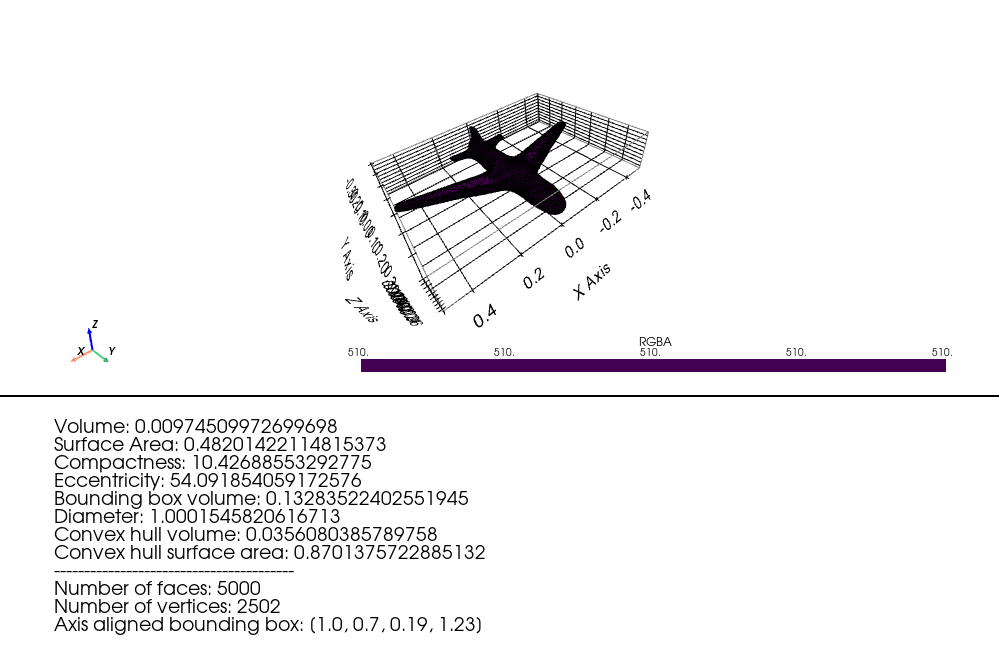
\includegraphics[width=\textwidth]{assets/feature_extraction/scalar_features/airplane.png}
        \caption{Airplane}
        \label{fig:airplane-scalars}
    \end{subfigure}
    \hfill
    \begin{subfigure}[b]{0.45\textwidth}
        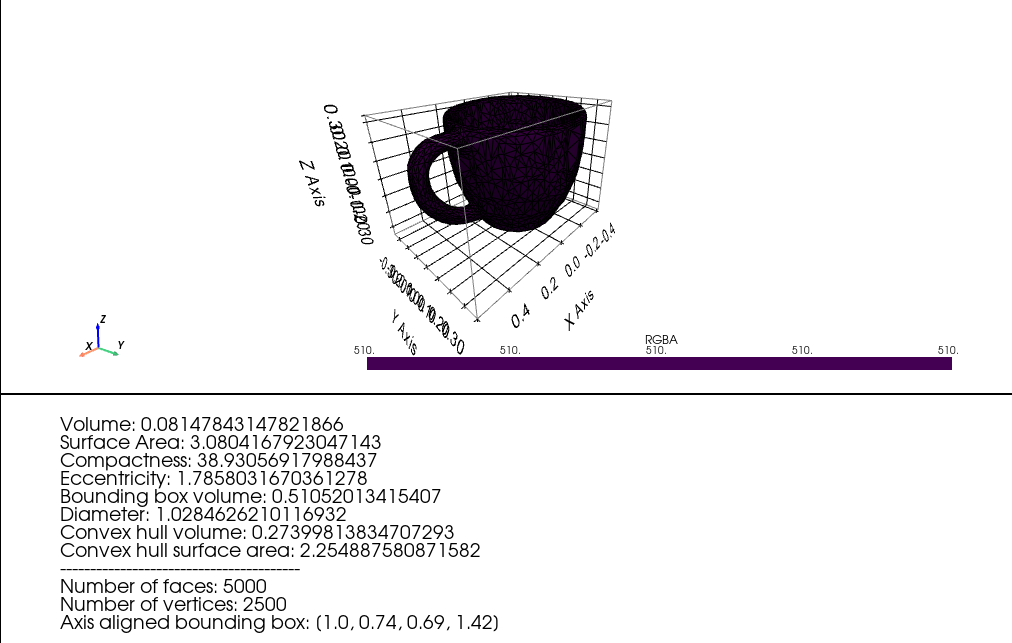
\includegraphics[width=\textwidth]{assets/feature_extraction/scalar_features/cup.png}
        \caption{Cup}
        \label{fig:cup-scalars}
    \end{subfigure}
    \hfill
    
    \begin{subfigure}[b]{0.45\textwidth}
        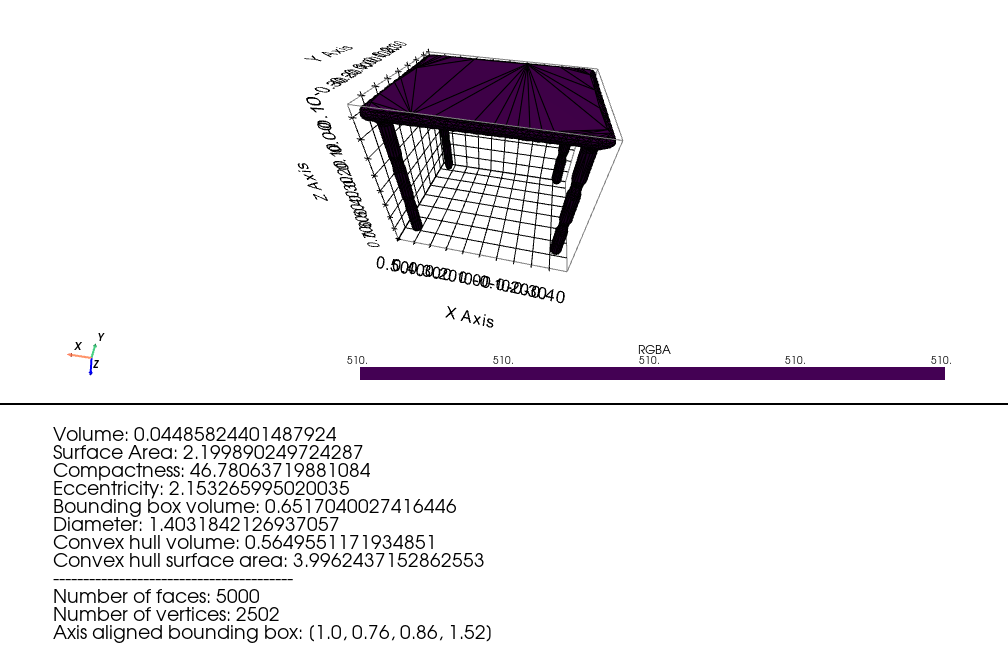
\includegraphics[width=\textwidth]{assets/feature_extraction/scalar_features/table.png}
        \caption{Table}
        \label{fig:table-scalars}
    \end{subfigure}
    \hfill
    \begin{subfigure}[b]{0.45\textwidth}
        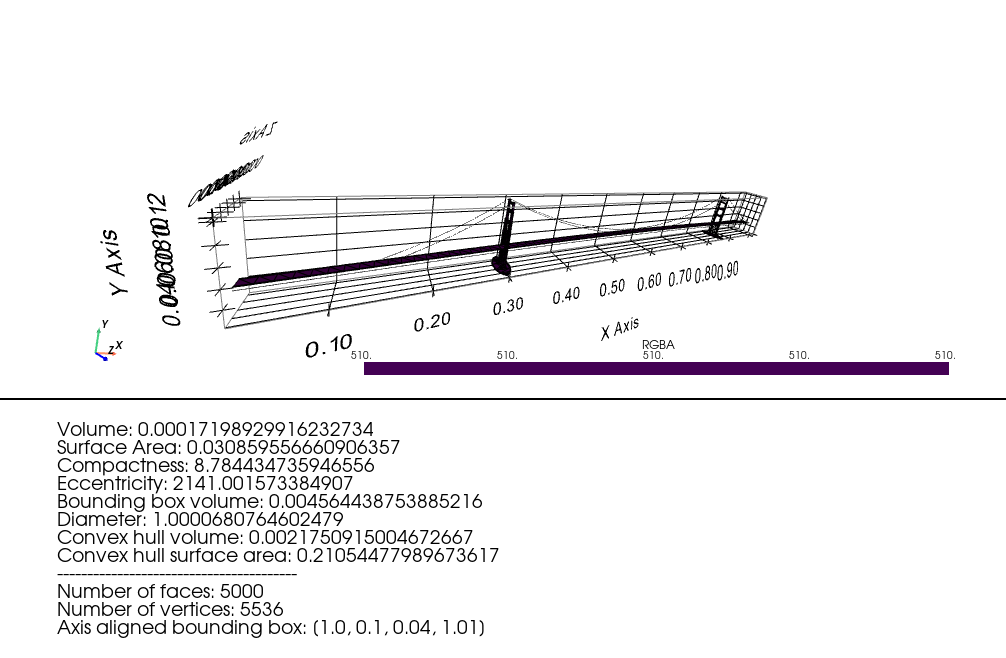
\includegraphics[width=\textwidth]{assets/feature_extraction/scalar_features/bridge.png}
        \caption{Bridge}
        \label{fig:bridge-scalars}
    \end{subfigure}
    \caption{Global descriptors for 3D shapes from our data set}
    \label{fig:global-descriptors-dataset}
\end{figure}

\section{Discriminating Shapes}
\label{section:discriminating-using-features}
The end goal of our retrieval system is that, when provided with a query shape, the system must find the most
shapes from our database that are most similar to it.
For this to happen, we have to determine the similarities - or rather, the dissimilarities - between the shapes in our
database and the query shape.
Instead of using the similarity to determine how similar shapes are, we use the dissimilarity to determine how dissimilar they are, because this is far easier to work with.
The dissimilarity between two shapes can be seen as the inverse notion of the similarity between two shapes.
We take this dissimilarity to be the distance between the feature vector representations of the shapes.
The intuition is that the lower this distance is between two shapes, the more similar these shapes are to each other.
Since our feature vector consists of many values and different types of data (i.e.\ scalars and histograms), we have to define a distance measure that is able to properly take all these values into account in order to distinguish between shapes accurately.
This section discusses how the features are normalized and how these normalized values are subsequently used for calculating distances between shapes.
We have implemented several ways of performing these normalizations and distance calculation tasks.
We will discuss which methods can be used and explain why we have chosen the default configuration that is used for the matching of shapes.

\subsection{Feature normalization}
The feature vectors contain many values, and all these values have different ranges.
If one feature has a far larger range of values than others, this feature would be dominant in determining whether shapes are similar.
So, in order to give equal power to all features, we have to normalize their values.
One way to achieve this goal is to use `Min-Max Normalization' to bring all values into the range of real numbers $[0, 1]$.
Given the minimum value $x_{min}^{f_s}$ and the maximum value $x_{max}^{f_s}$ for a scalar feature ${f_s}$ a value $x_i^{f_s}$ of that given feature is standardized following the formula
\begin{equation}
    x_i^{f'_s} = \frac{x_i^{f_s} - x_{min}^{f_s}}{x_{max}^{f_s} - x_{min}^{f_s}}.
\end{equation} 
This normalization method subtracts the minimum value from each value before dividing them by the complete range of values, the maximum value minus the minimum value, to get values ranging between $0$ and $1$.
Next to `min-max normalization', our system provides the user with the option to choose `z-score normalization'.
This normalization method standardizes, again for a scalar feature ${f_s}$, a value $x_i^{f_s}$ using the formula
\begin{equation}
    x_i^{f'_s} = \frac{x_i^{f_s} - x_{avg}^{f_s}}{x_{stddev}^{f_s}},
\end{equation} 
where $x_{avg}^{f_s}$ is the average value and $x_{stddev}^{f_s}$ is the standard deviation for the feature ${f_s}$.
Here the average value is subtracted from all values before dividing by the standard deviation for that value.
This generally does not bring all values in the range of real numbers $[0, 1]$.
However, most values will be contained either in or just outside that range (i.e.\ 95\% of the time the values will be in range $[0,1]$).
If there are significant outliers, these will also be far outside this range.
It is up to the user whether this is wanted or not.

The normalization discussed so far, the `min-max normalization' and the `z-score normalization', only applies to the scalar features.
The values for the histograms of the local descriptors are normalized separately because it does not make sense to perform the same normalization on these features.
For these histograms, the bin values are divided by the sum of the bin values for that feature, such that the area of the histogram/distribution is equal to $1$.
Mathematically, given a histogram feature $f_h$ with bin values $b_1^{f_h}, b_2^{f_h}, \dots, b_n^{f_h}$, the normalized bin values are calculated with
\begin{equation}
    b_i^{f'_h} = \frac{b_i^{f_h}}{\sum_{j=1}^n b_j^{f_h}}.
\end{equation}
This normalization is performed on each histogram feature separately.

\subsection{Distance calculation}
Using the normalized feature values, we can calculate a distance between feature vectors using some distance function.
An overview of the definitions for the implemented distance measures can be found in Table \ref{tab:distance-functions}.
In addition to their general formulas, we have also specified some advantages of the different distance measures.
The distance functions are also included in the table containing the global notations, Table \ref{tab:notations}.
In the following subsection we will discuss these distance measures in more detail and explain the weighing that is
performed as part of the distance calculations.

Firstly, we will talk about the weighing that is performed for the features.
Then, we will discuss the distance functions that can be used for both the scalar features and the histogram
features separately.
Finally, we will the reasoning behind our choices for the default values and distance functions we use in the final
system.

\begin{table}[ht]
    \centering
    \resizebox{\textwidth}{!}{
        \begin{tabular}{c|c|c}
            Distance Name & Formula & Advantages \\
            \hline
            
            \multirow{2}{*}{LP norm} & $L_p(\overrightarrow{x},\overrightarrow{y}) = \left( \sum_{i = 1}^n \left| x_i - y_i \right| ^p \right)^{\frac{1}{p}}$ & \multirow{2}{*}{Easy to compute} \\
            & $L_{\infty}(\overrightarrow{x},\overrightarrow{y}) = \max\limits_{i \in \{1, \dots , n\}} \left| x_i - y_i \right|$ & \\
            \hline

            Cosine distance & $d_{cos}(\overrightarrow{x}, \overrightarrow{y}) = 1 - \frac{\overrightarrow{x} \cdot \overrightarrow{y}}{||\overrightarrow{x}||\cdot ||\overrightarrow{y}||}$ & Easy to compute, Scale Invariant \\
            \hline
            Mahalanobis Distance & $d_{mahalanobis}(\overrightarrow{x}, \overrightarrow{y}) = \sqrt{(\overrightarrow{x} - \overrightarrow{y})^T Cov^{-1}(X) (\overrightarrow{x} - \overrightarrow{y})}$ & Accounts for correlations between features \\
            \hline
            \multirow{2}{*}{Earth's Mover's Distance} & \multirow{2}{*}{$emd(A,B) = \min \sum_{a \in A} \sum_{b \in B} f_{a, b} d_{a, b}$} & Applicable on histograms, Intuitive \\
            & & Measure on full distribution range \\
            \hline
            \multirow{2}{*}{Kullback-Leibler Divergence} & \multirow{2}{*}{$d_{KL}(A, B) = \sum_{i=1}^n (a_i - b_i) \log \left( \frac{a_i}{b_i} \right)$} & Applicable on histograms \\
            & & Measures shared information \\
        \end{tabular}
    }
    \caption{Distance functions}
    \label{tab:distance-functions}
\end{table}

\subsubsection{Feature weighing}
Each feature in the feature vector measures a certain aspect/property of the shape.
It is important to note that, while some features might measure totally different, independent, aspects of the shape,
other features could have a lot of overlap in what they measure.
Moreover, some features might be more informative than others, especially for certain classes.
Due to this, we chose to add the ability to weigh every feature by a certain user-chosen factor.
When these weights are not specified by the user, we simply apply an equal weighing across the feature vector.

We perform two kinds of weighing - weighing of the global features, and weighing between the importance of the distance
calculated from the global features and the distances of the local features.

By default, the values of the global features are weighed equally with weights of $1$, so this actually leaves the
distance calculation for the scalar features unweighted.
But, if the user considers it necessary, there is a possibility to assign an individual weight to each global feature.
However, this weight assignment is dependent on the distance function that is used to calculate the distance between
the scalar values.
Therefore, we will discuss this scalar weighing together with the distance measures used for the scalar features, in
section \ref{subsubsec:scalar_distance}.

We calculate one distance over the scalar features and one distance per each histogram feature.
Since we are using five histogram features, we end up with a total of six distances between two shapes.
The final distance is calculated as a weighted sum of these distances.
This weighing is simply

\begin{equation}
    \begin{aligned}[b]
    & d_{final}(\overrightarrow{x}, \overrightarrow{y}) = w_{scalar} d_{scalar}(\overrightarrow{x}, \overrightarrow{y}) + w_{A_3} d_{A_3}(\overrightarrow{x}, \overrightarrow{y}) + \\
    & + w_{D_1} d_{D_1}(\overrightarrow{x}, \overrightarrow{y}) + w_{D_2} d_{D_2}(\overrightarrow{x}, \overrightarrow{y}) + w_{D_3} d_{D_3}(\overrightarrow{x}, \overrightarrow{y}) + w_{D_4} d_{D_4}(\overrightarrow{x}, \overrightarrow{y}) \\
    \end{aligned}
    \label{eq:weighing}
\end{equation}

where we can assign a value to the weight of every single distance - both for the scalar distance and for each histogram feature.
By default, we use the weights $w_{scalar} = 3$ and $w_{A_3} = w_{D_1} = w_{D_2} = w_{D_3} = w_{D_4} = 1$.
This weighing makes the distance between the global features three times more important than the distance between local descriptors.
To balance this, the local descriptors all-together have a higher weight than the scalar features - a weight of $5$ versus a weight of $3$.

\subsubsection{Distance between global features}\label{subsubsec:scalar_distance}
For the scalar values, we can calculate their distance using Minkowski distances, or the LP norm, like the well-known
and often used $L_1$ or $L_2$ metrics, which are also known as the Manhattan and Euclidean distance respectively.
These distances are defined as
\begin{equation}
    L_p(\overrightarrow{x}, \overrightarrow{y}) = \left( \sum_{i = 1}^n w_i \left| x_i - y_i \right|^p \right)^\frac{1}{p}\label{eq:lpdistance}
\end{equation}
where $\overrightarrow{x} = {x_1, \dots, x_n}$ and $\overrightarrow{y} = {y_1, \dots, y_n}$ are the feature vectors between which this distance is calculated, and $\overrightarrow{w} = {w_1, \dots, w_n}$ are the weights that we apply to the scalar values.
We have implemented both these $L_1$ and $L_2$ metrics, as well as the $L_{\infty}$ distance.

This $L_{\infty}$ is the LP norm corresponding to the limit where $p$ converges to $\infty$, and is therefore
calculated slightly differently, as
\begin{equation}
    L_{\infty}(\overrightarrow{x}, \overrightarrow{y}) =  \max\limits_{i \in \{
    1, \dots, n\}} w_i \left| x_i - y_i \right|,
\end{equation}
with $\overrightarrow{x} = {x_1, \dots, x_n}$, $\overrightarrow{y} = {y_1, \dots, y_n}$ and $\overrightarrow{w} = {w_1, \dots, w_n}$ defined as in \ref{eq:lpdistance}.

Apart from the $L$ metric distances, we have also implemented the cosine distance and the Mahalanobis distance.
The cosine distance is useful to determine how different vectors are based on the angle between them.
As a result, this metric is independent of the length of the vectors.
The cosine distance is defined as $1$ minus the cosine similarity, which is the value $cos(\theta)$ with $\theta$ the angle between the vectors.
Therefore, the cosine distance is defined as
\begin{equation}
    d_{cos}(\overrightarrow{x}, \overrightarrow{y}) = 1 - \frac{\overrightarrow{w} \cdot\overrightarrow{x} \cdot \overrightarrow{y}}{\sqrt{\overrightarrow{w} \cdot\overrightarrow{x} \cdot \overrightarrow{x}} \cdot \sqrt{\overrightarrow{w} \cdot\overrightarrow{y} \cdot \overrightarrow{y}}}.
\end{equation}

Lastly, we have also implemented the Mahalanobis distance.
This metric gives a distance between two vectors with respect to a probability distribution.
The Mahalanobis distance accounts for the correlation between features by using the covariance matrix in its formula.
The definition is somewhat similar to the Euclidean distance, where these distances coincide when this covariance matrix is the identity matrix.
The definition of the Mahalanobis distance is
\begin{equation}
    d_{mahalanobis}(\overrightarrow{x}, \overrightarrow{y}) = \sqrt{(\overrightarrow{x} - \overrightarrow{y})^T Cov^{-1}(X) (\overrightarrow{x} - \overrightarrow{y})},
\end{equation}
where $X$ is the set of the scalar part of all the feature vectors in our database, $\overrightarrow{x}, \overrightarrow{y} \in X$.
Notice that this distance does not require any weighting.
Rather, the weighting is performed by means of the covariance matrix.

\subsubsection{Distance between local (histogram) features}\label{subsubsec:hist_distance}
Weighing the feature distances in the final distance calculation is not enough to properly deal with the histogram
features - the features corresponding to the local descriptors.
Simply using the same distance measure as for the scalars does not make sense for the histogram features, which is why
we must handle them separately from the scalar features.

Consider that the feature values corresponding to one local descriptor together form a feature.
Therefore, for one such local descriptor we have to use the full range of values in order to determine a relevant
distance, instead of comparing value by value like we do for the scalar values.

Since the values of a histogram feature represent the bins of a distribution, we can calculate the Earth's Mover
Distance (EMD) \cite{rubner_emd_2000} between two histograms.
This distance function measures the amount of work that is needed to transform one distribution into another one,
which gives a meaningful distance measure between two histograms corresponding to the same local descriptor.

The EMD measure is defined as the minimum work that is needed to move from one distribution to the other.
Since we are working with histograms with equal amounts of bins representing the same bin ranges, this distance calculation is a simplified version of the general case.
Define $f_{a, b}$ as the amount that is moved from bin $a$ of histogram $A$ to bin $b$ of histogram $B$.
Furthermore, define $d_{a, b}$ as the distance between the ranges of values of bin $a$ of histogram $A$ and bin $b$ of histogram $B$.
Then the Earth's Mover's Distance is defined as
\begin{equation}
    emd(A,B) = \min \frac{\sum_{a \in A} \sum_{b \in B} f_{a, b} d_{a, b}}{\sum_{a \in A} \sum_{b \in B} f_{a, b}}.
\end{equation}
Instead of an exhaustive search over all possible solutions, much smarter approaches can be made in order to calculate this distance.
We used the implementation by the $scipy.stats$ library in order to calculate this efficiently.
In this implementation this distance is called the Wasserstein distance, which is a different name for the EMD.

This is the default distance measure that is used for calculating distances between histograms.
In addition to EMD, we also implemented, the Kullback-Leibler Divergence \cite{kullback1951information} and in the final system allow the user to specify it as the distance measure for local descriptors.
The Kullback-Leibler Divergence - also called the relative entropy, measures the relative entropy between two distributions.
It expresses how surprising one distribution is given we expect the other distribution.
It therefore somewhat measures how much information the two distributions share.

The measure that we implement is not exactly this relative entropy, since we add the distance in the reverse direction to the calculated distance in order to make the distance symmetric.
That is
\begin{equation}
    d_{KL}(A, B) = d_{KL}^{pure}(A, B) + d_{KL}^{pure}(B, A),
\end{equation}
where $d_{KL}$ denotes our implementation of the Kullback-Leibler Divergence, and $d_{KL}^{pure}$ is the original (pure) Kullback-Leibler Divergence.
The formula for our implementation is
\begin{equation}
    d_{KL}(A, B) = \sum_{i=1}^n (a_i - b_i) \log \left( \frac{a_i}{b_i} \right).\label{eq:kl-d}
\end{equation}

\subsection{Motivation for default distance measures}
In the scalar feature normalization, we have opted for using the `z-score' normalization.
We use this as the default since this normalization method is much more invariant to outliers, in comparison to `min-max' normalization, which is heavily affected by outliers.
Moreover, for shapes that are not in our data set, we need to compute the feature vector on the fly, and it could be the case that applying a min-max normalization with the minimum and maximum values from our data set would lead to values outside the [0,1] range.
For the histogram features, there is only one appropriate option for normalization, which is the bin normalization discussed in the corresponding section.
This is also the only option implemented in our tool.

We have chosen the cosine distance for calculating the distance for the scalar values since this distance measure is not affected by the length of the feature values.
It is only dependent on the feature values relative to each other, giving a fair calculation across all features in the feature vector.
Using the cosine distance, features with large value ranges, which can still happen even after normalization, will not dominate the distance calculation.

For the distance calculation with respect to the local features, we have chosen the EMD measure, since this gives a more intuitive difference between two distributions.
Moreover, the EMD measure is a metric, whereas the (pure) Kullback-Leibler Divergence is not, since it does not satisfy the symmetry condition and the triangle inequality.
The symmetry condition is forced onto the measure in our implementation, as outlined in Equation \ref{eq:kl-d}.

In the final system, the default measures used are the cosine distance for the global features and the EMD for the local features.
These distances are weighed following Equation \ref{eq:weighing} to get our final distance measure.
The final measure is what determines how similar/dissimilar two shapes are.

%\subsection{Matching output}
%With the above defined distances we can perform matching on the 3D models. An example of this can be found in Figure \ref{fig:query-response-example}, where several query shapes are shown together with the five shapes that are found most similar to them. Furthermore we can show the feature vectors in 2D using dimensionality reduction. The output of this can be seen in Figure \ref{fig:feature-vectors-2D}.

\section{Scalability}
\label{section:scalability}
We take several approaches to improve the system's performance at scale.
First, consider that we store all of the features we extracted for the shapes from our database (See Figure \ref{fig:mr-pipeline}).
Therefore, when a new shape is queried, we first search for it in our data set.
If it is found, we will not need to preprocess it and compute features for it, since they are already in the database.
Only in the case where the query shape is not found in the database, do we preprocess it and compute its feature vector.

Our implementation of the computation of the distance function (See Sections \ref{subsubsec:scalar_distance} \& \ref{subsubsec:hist_distance}) is linear in terms of the number
of shapes in the database (i.e. $O(N)$, where $N$ is the number of feature vectors).
This complexity is good for small databases (in the thousands), but does not scale well as the number of shapes increases.
An improvement would be to achieve a sublinear complexity.
In the following two subsections we discuss two ways we go about doing so.

\subsection{A decision trees-based index}
To achieve sublinear time complexity for querying a database, an often-used approach is to precompute an index (i.e.\ a tree or a set of trees) that partitions the database.
An informed querying can then be made, based on that index.
We take this approach and compute an index that is composed of $500$ trees using the Approximate Nearest Neighbours (ANN) technique.
We further refer to the search using the precomputed index as $ANN$, and the search using our custom distance function, outlined in \ref{section:discriminating-using-features}, as $KNN$ (where $K$ stands for the $k$ nearest shapes returned on querying).

\paragraph{ANN}
This approach is considering the geometric properties of the $n$-dimensional space to compute a partition of the feature vector space.
We would guide the reader to \cite{rp_trees, ann} for an in-depth overview of how the index is computed.
The implementation we use is the one in the \ref{Annoy_t} package.
It creates an accurate tree, with a trade-off between accuracy and the final size of the stored tree.
Since our database is small compared to the size that the \ref{Annoy_t} implementation is intended for (i.e.\ Spotify), this is not a large worry for us.
To compute an accurate index, we use $500$ trees and the final index file size is $>5mb$.

There is another limitation with this approach however - namely that not all distance functions can be used for computing the index.
The distance functions we implemented, and we can use, are the $L_p$ metrics and cosine distance (described in Section \ref{subsubsec:scalar_distance}).

Because some distance functions perform a normalization as part of their calculation, and we want to allow the user to choose between them in the final system, we store the pre-normalized scalar features in our database.
We precompute the ANN index with these un-normalized scalar feature values.
Note from Figures \ref{fig:A3-signatures-1} to \ref{fig:D4-signatures-2}, that for the majority of the classes, the histograms tend to have a lot of zeros in them.
Therefore, the vectors of the features are both very high-dimensional and sparse.
Due to these reasons, the cosine similarity is preferred over the $L_p$ metrics when computing our index.

\subsubsection{Results}
To quantify our theoretical discussion and evaluate our approach, we performed a set of experiments.
We ran both the basic, $O(N)$, approach and the index-based, $O(log (N))$, approach on 400 shapes from our data set and recorded the CPU runtime taken for each shape.
In Table \ref{tab:environment-knn-vs-ann} we show the configuration of the machine we run our experiments on.
The results of the first experiment are presented in Figure \ref{fig:ann-vs-knn-run-times}.
Observe that the index-based approach, denoted as ANN, is an order of magnitude faster than the basic KNN approach.
For the second experiment, we used a set of 3 randomly picked shapes and performed the query using both the ANN approach (Figure \ref{fig:query-response-example-ann}) and the KNN approach (Figure \ref{fig:query-response-example}).
As one might notice, the results are very poor for the ANN approach, however, this does not mean that this approach is giving poor results in general.
Moreover, for some shapes, the ANN (i.e.\ index based) approach is even performing better than the custom function approach (See Figure \ref{fig:query-response-example-ann-good}).
Notice how for a teddy bear, the ANN approach is returning only teddy bears, whilst the custom function approach is returning a chair and a spider as well.

\begin{table}[H]
    \centering
    \begin{tabular}{c|c}
        Characteristic & Value \\
        \hline
        Architecture &                    x86\_64 \\
        CPU op-mode(s) &                  32-bit, 64-bit \\
        Address sizes &                   39 bits physical, 48 bits virtual \\
        CPU(s)&                          4 \\
        Thread(s) per core &              2 \\
        Core(s) per socket&              2 \\
        Socket(s)&                       1 \\
        NUMA node(s)&                    1 \\
        Vendor ID&                       GenuineIntel \\
        CPU family&                      6 \\
        Model&                           142 \\
        Model name&                      Intel(R) Core(TM) i7-7500U CPU @ 2.70GHz \\
        Stepping&                        9 \\
        CPU MHz&                         3500 \\
        CPU max MHz&                     3500 \\
        CPU min MHz&                     400 \\
    \end{tabular}
    \caption{Information about the machine on which the experiments were performed}
    \label{tab:environment-knn-vs-ann}
\end{table}


\begin{figure}[H]
    \centering
    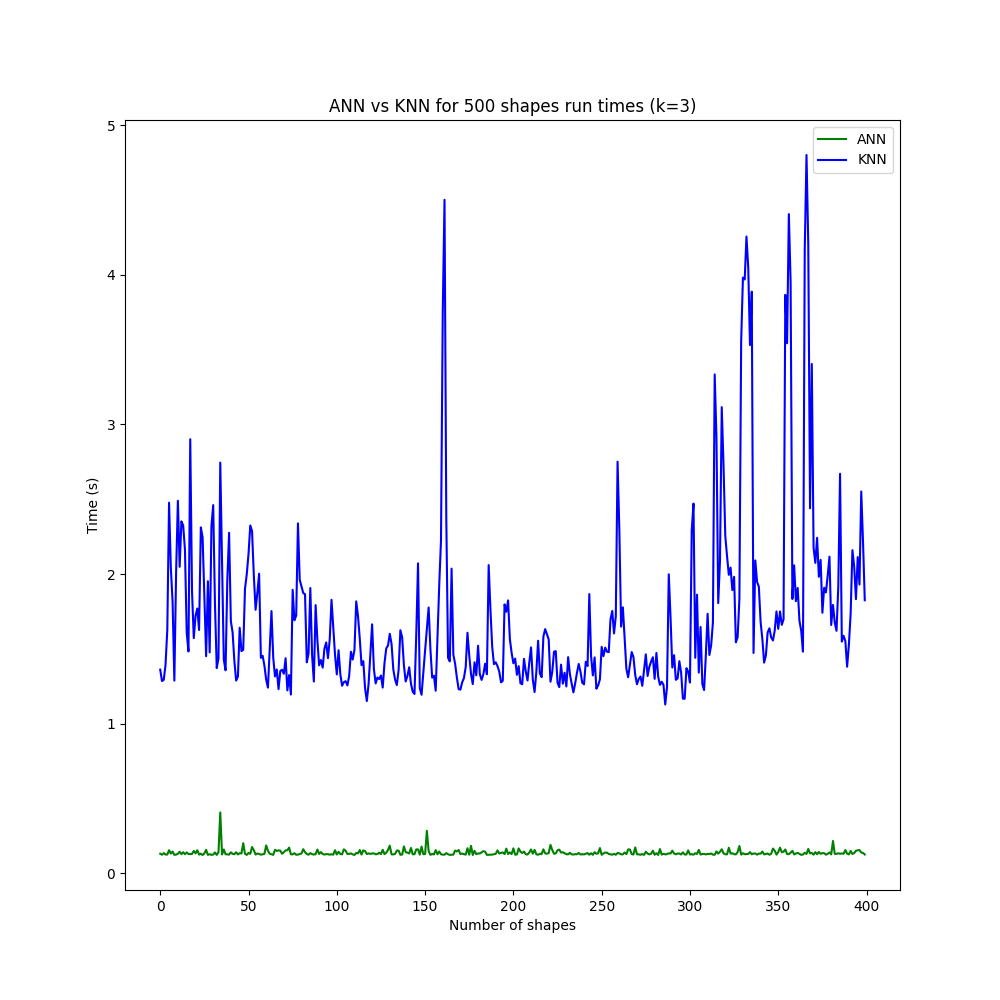
\includegraphics[width = 0.5\textwidth]{assets/evaluation_results/ANN_vs_KNN_run_time.png}
    \caption{ANN vs KNN in terms of run times (k=3)}
    \label{fig:ann-vs-knn-run-times}
\end{figure}


\begin{figure}[H]
    \centering

    \begin{subfigure}[b]{0.3\textwidth}
        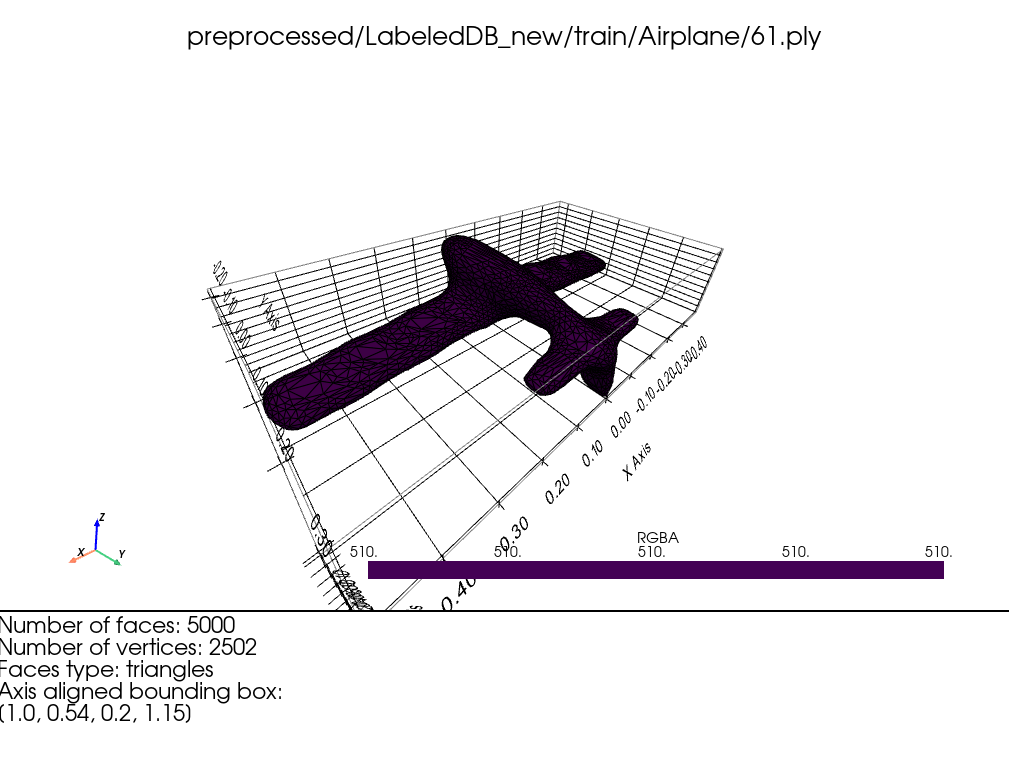
\includegraphics[width=\textwidth]{assets/queries/airplane/input.png}
        \caption{Query input \newline}
        \label{fig:query-input-knn-1}
    \end{subfigure}
    \hfill
    \begin{subfigure}[b]{0.65\textwidth}
        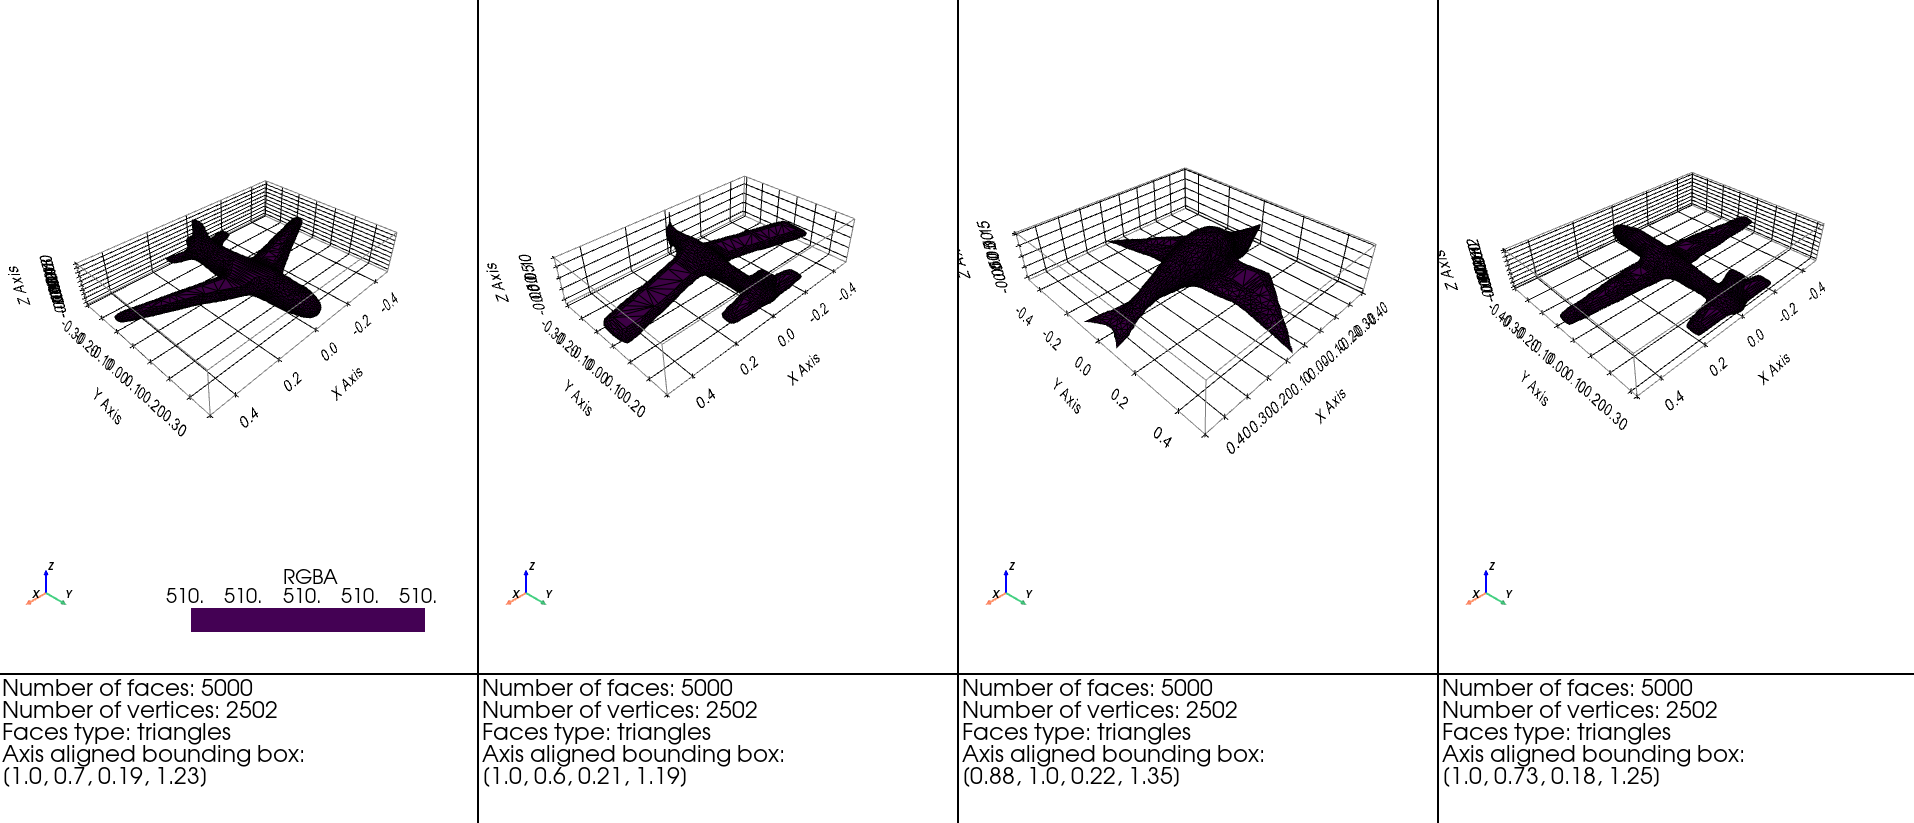
\includegraphics[width=\textwidth]{assets/queries/airplane/output.png}
        \caption{Query output; Respective distances: $7.651\cdot10^{-5}, 8.359\cdot10^{-5}, 9.412\cdot10^{-5}, 10.658\cdot10^{-5}$ }
        \label{fig:query-output-knn-1}
    \end{subfigure}
    \hfill

    \begin{subfigure}[b]{0.3\textwidth}
        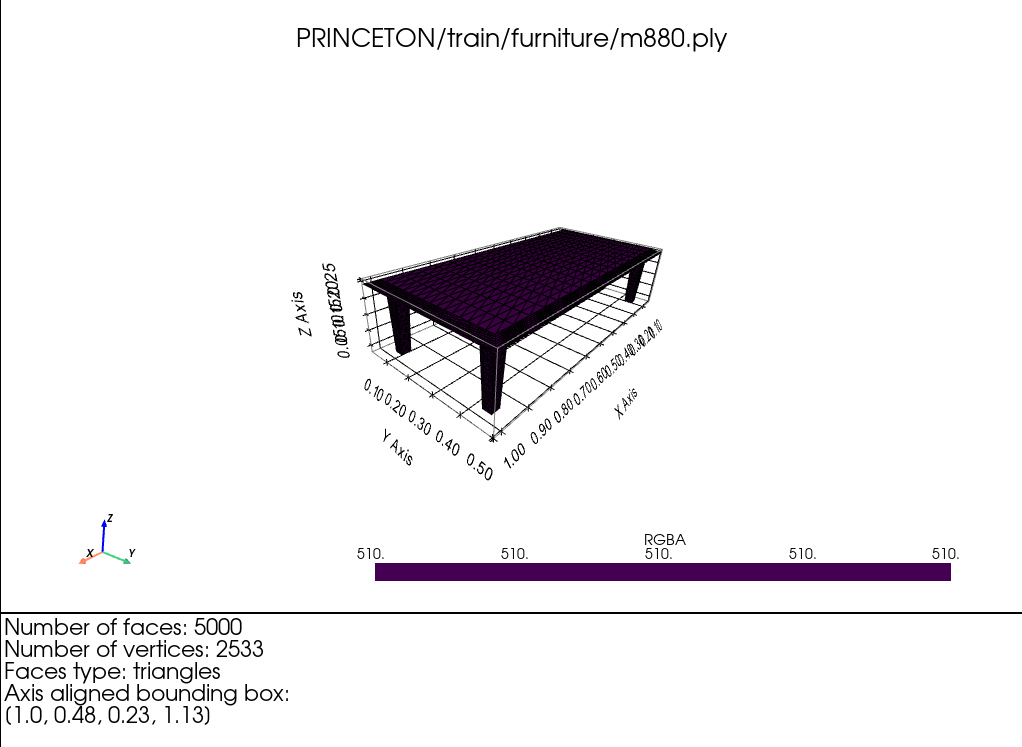
\includegraphics[width=\textwidth]{assets/queries/furniture/input.png}
        \caption{Query input}
        \label{fig:query-input-knn-2}
    \end{subfigure}
    \hfill
    \begin{subfigure}[b]{0.65\textwidth}
        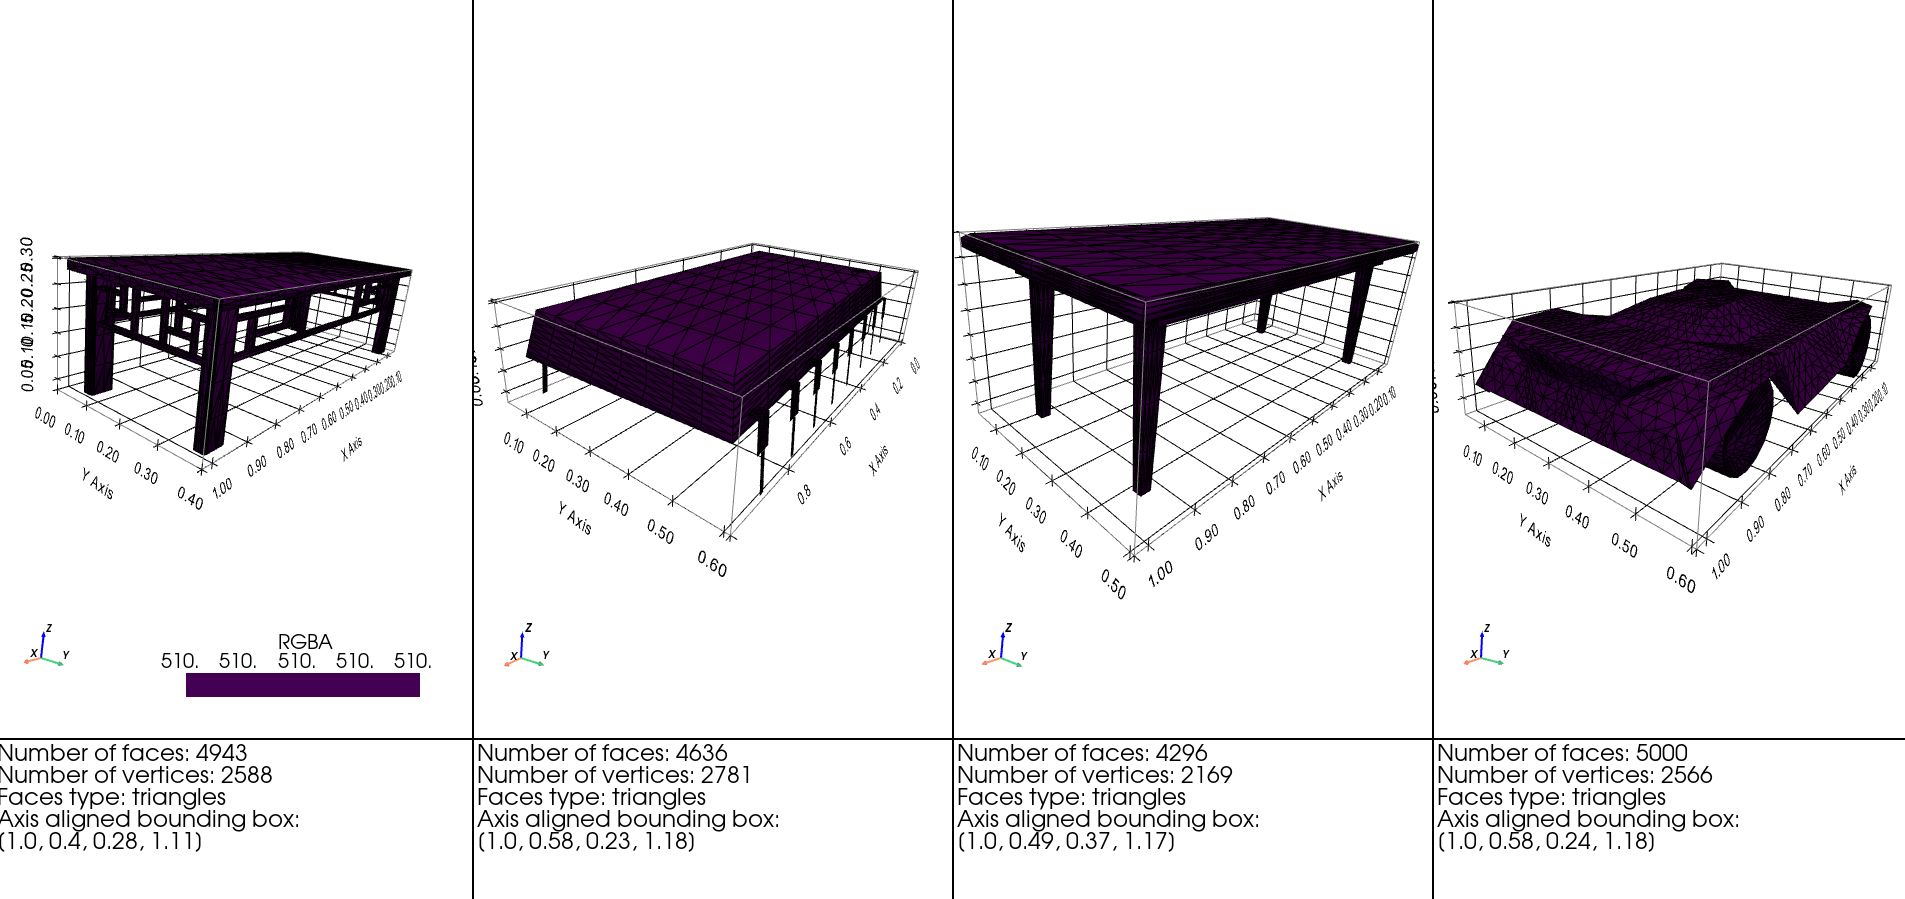
\includegraphics[width=\textwidth]{assets/queries/furniture/output.png}
        \caption{Query output; Respective distances: $ 16.322\cdot10^{-5}, 16.381\cdot10^{-5}, 17.903\cdot10^{-5}, 18.798\cdot10^{-5}$}
        \label{fig:query-output-knn-2}
    \end{subfigure}
    \hfill
    
    \begin{subfigure}[b]{0.3\textwidth}
        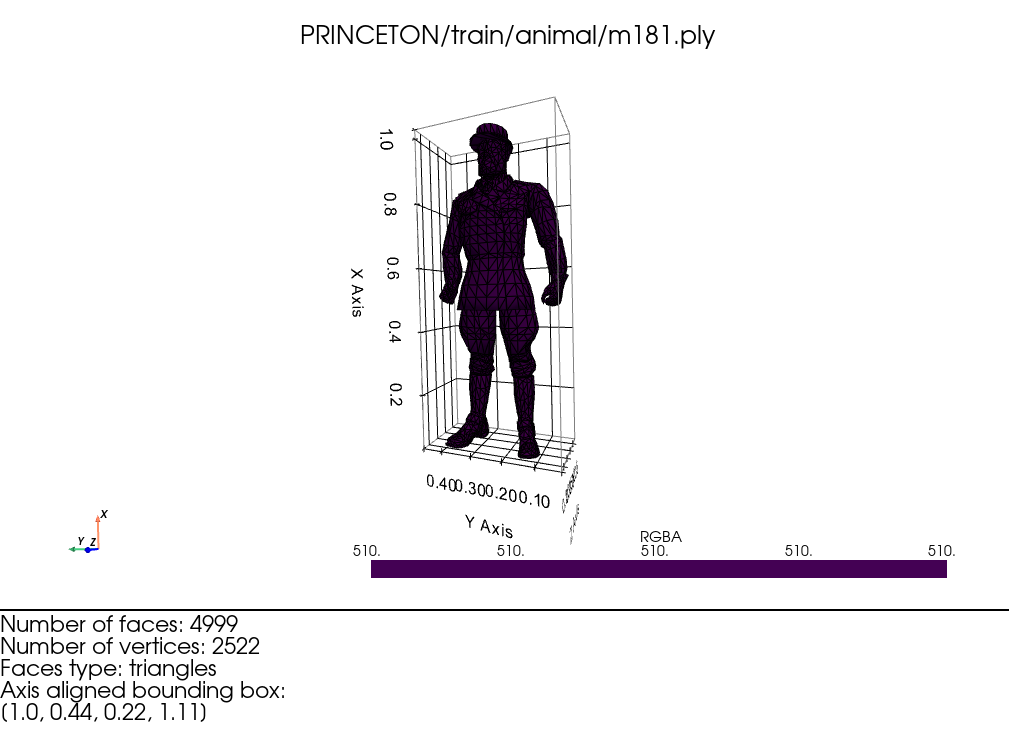
\includegraphics[width=\textwidth]{assets/queries/human/input.png}
        \caption{Query input}
        \label{fig:query-input-knn-3}
    \end{subfigure}
    \hfill
    \begin{subfigure}[b]{0.65\textwidth}
        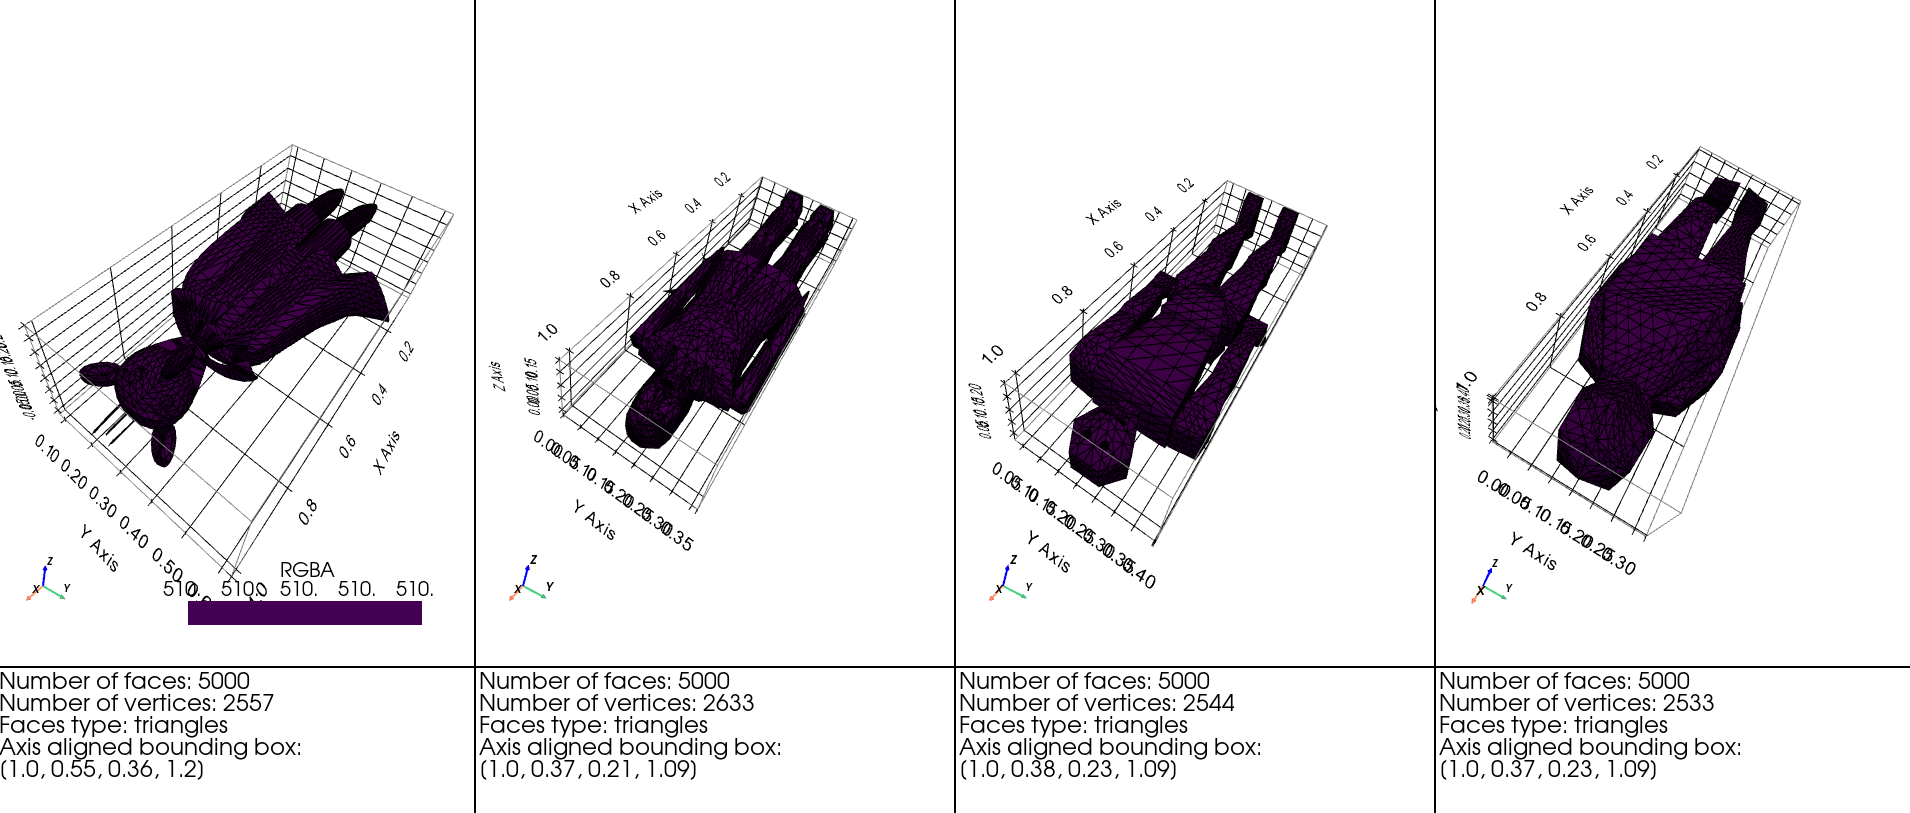
\includegraphics[width=\textwidth]{assets/queries/human/output.png}
        \caption{Query output; Respective distances: $10.354\cdot10^{-5}, 10.799\cdot10^{-5}, 12.264\cdot10^{-5}, 13.187\cdot10^{-5}$}
        \label{fig:query-output-knn-3}
    \end{subfigure}
    \hfill
    
    \caption{Example of the query response using KNN}
    \label{fig:query-response-example}
\end{figure}


\begin{figure}[H]
    \centering
    \begin{subfigure}[b]{0.3\textwidth}
        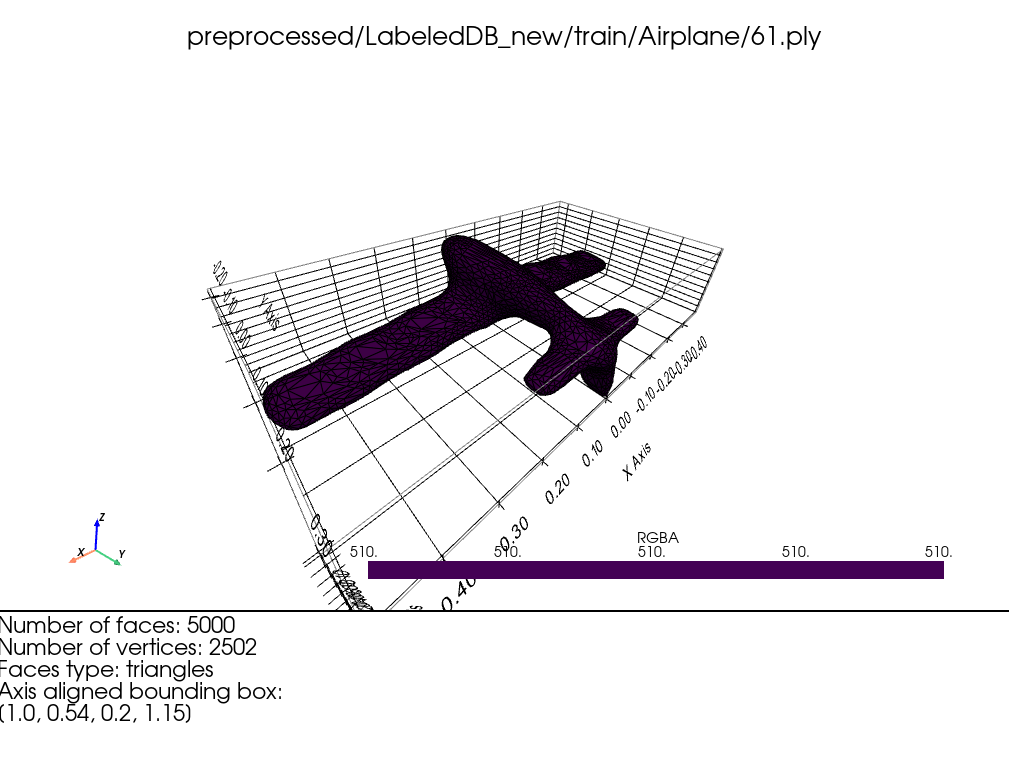
\includegraphics[width=\textwidth]{assets/queries/airplane/input.png}
        \caption{Query input}
        \label{fig:query-input-ann-1}
    \end{subfigure}
    \hfill
    \begin{subfigure}[b]{0.65\textwidth}
        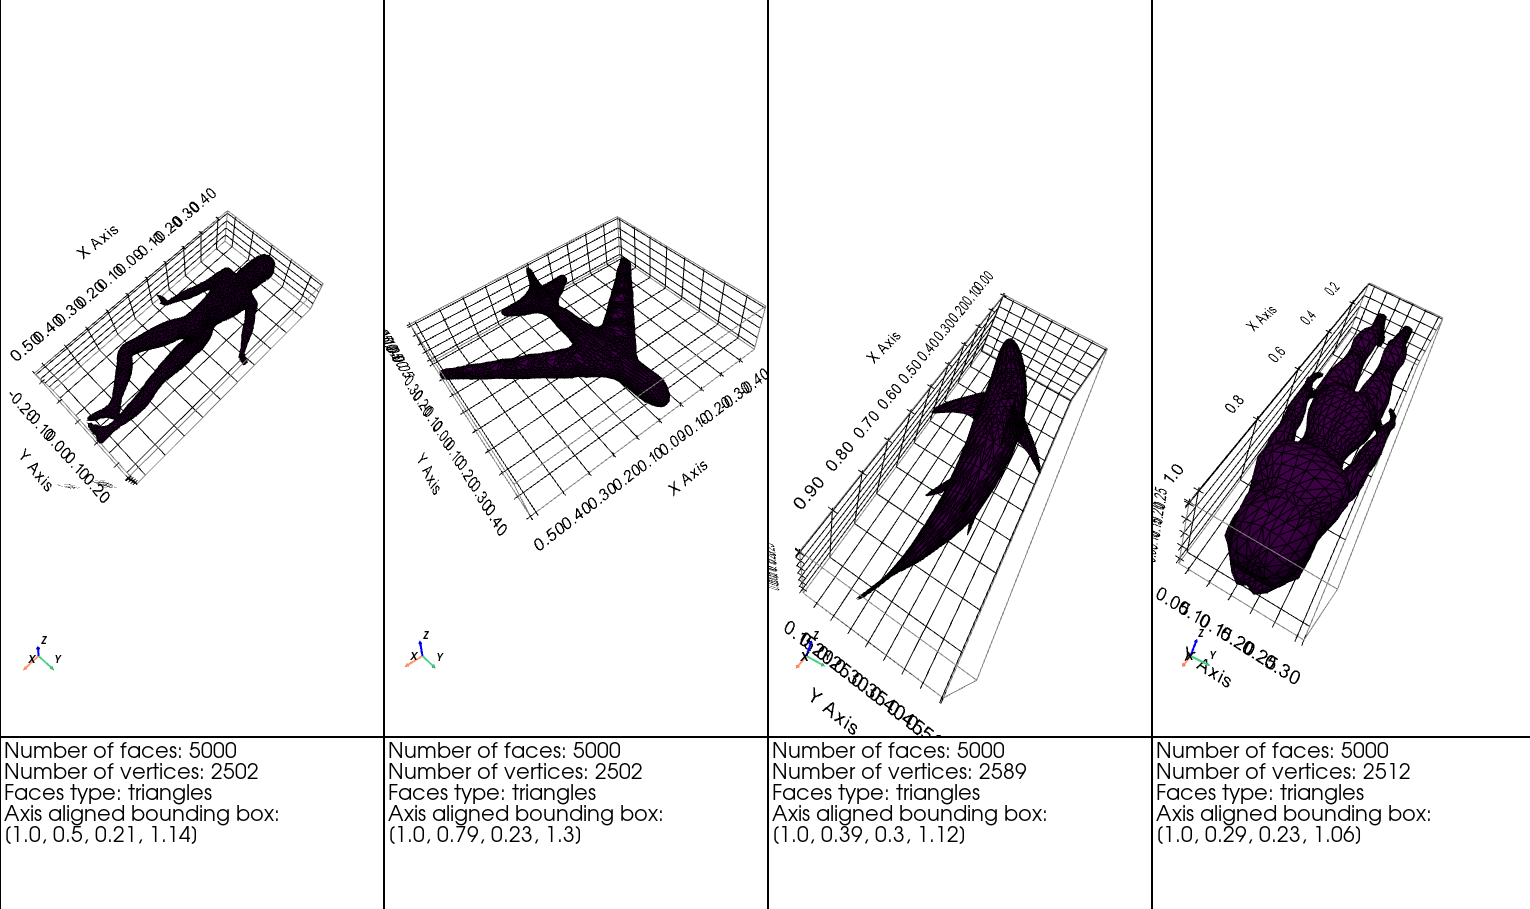
\includegraphics[width=\textwidth]{assets/queries/airplane_ann/output.png}
        \caption{Query output; Respective distances: 0.010, 0.015, 0.018, 0.021}
        \label{fig:query-output-ann-1}
    \end{subfigure}
    \hfill
    
    \begin{subfigure}[b]{0.3\textwidth}
        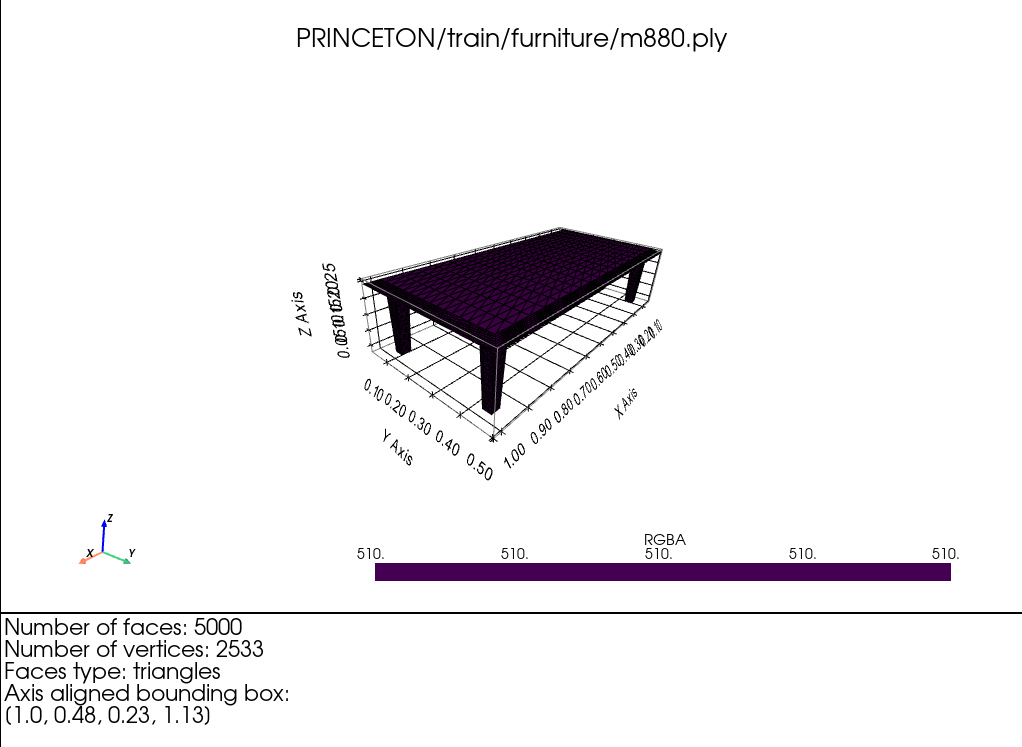
\includegraphics[width=\textwidth]{assets/queries/furniture/input.png}
        \caption{Query input}
        \label{fig:query-input-ann-2}
    \end{subfigure}
    \hfill
    \begin{subfigure}[b]{0.65\textwidth}
        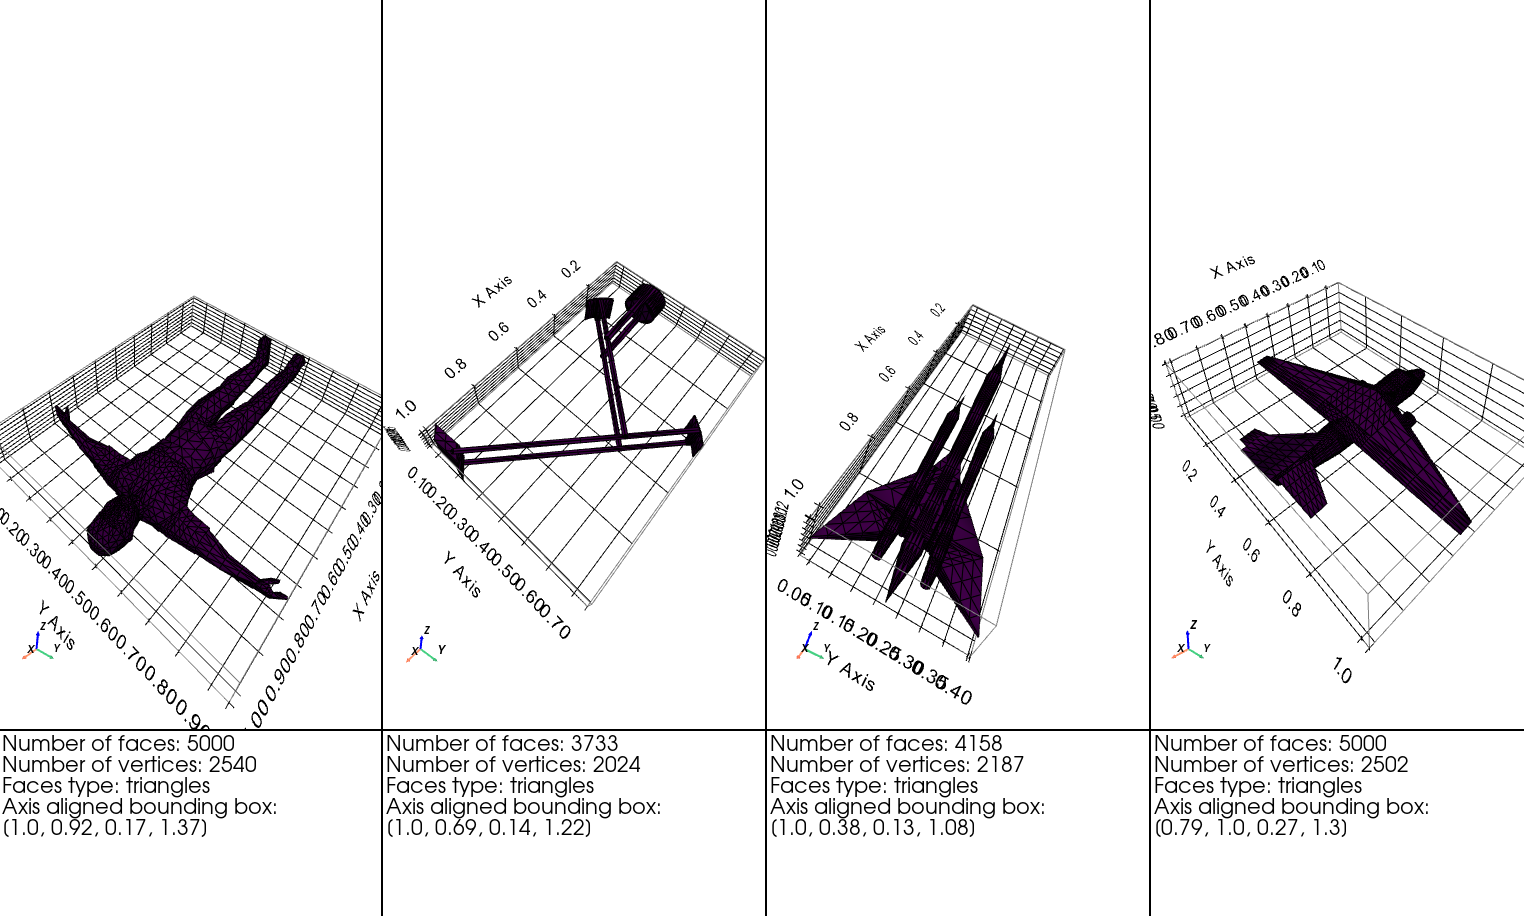
\includegraphics[width=\textwidth]{assets/queries/furniture_ann/output.png}
        \caption{Query output; Respective distances: 0.007, 0.013, 0.015, 0.019}
        \label{fig:query-output-ann-2}
    \end{subfigure}
    \hfill
    
    \begin{subfigure}[b]{0.3\textwidth}
        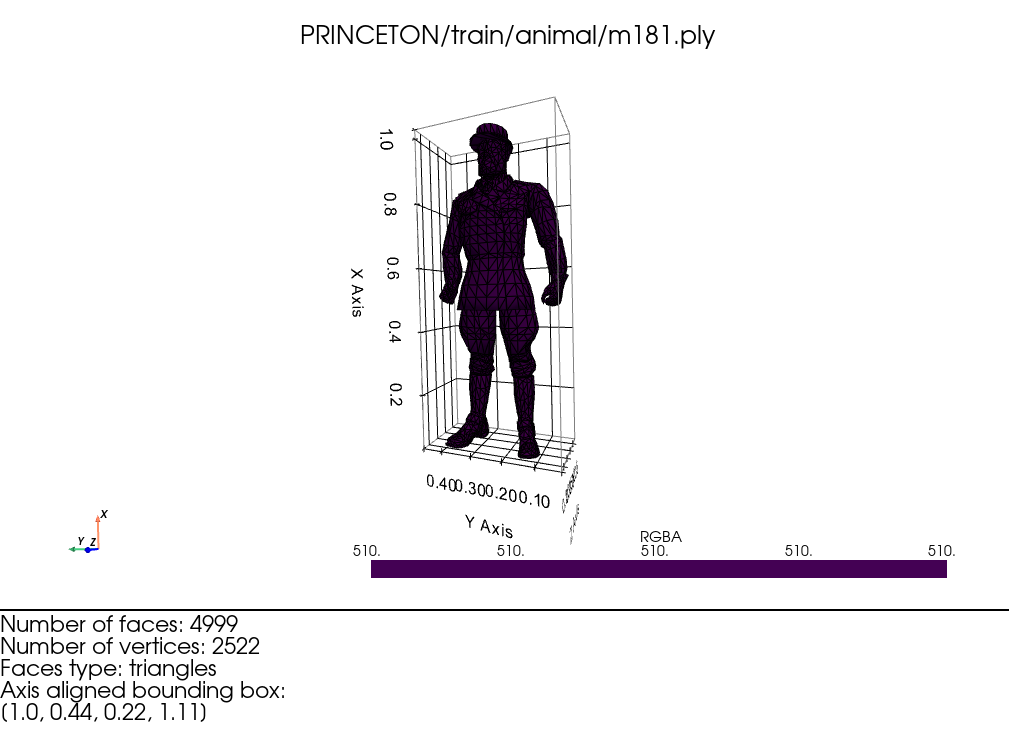
\includegraphics[width=\textwidth]{assets/queries/human/input.png}
        \caption{Query input}
        \label{fig:query-input-ann-3}
    \end{subfigure}
    \hfill
    \begin{subfigure}[b]{0.65\textwidth}
        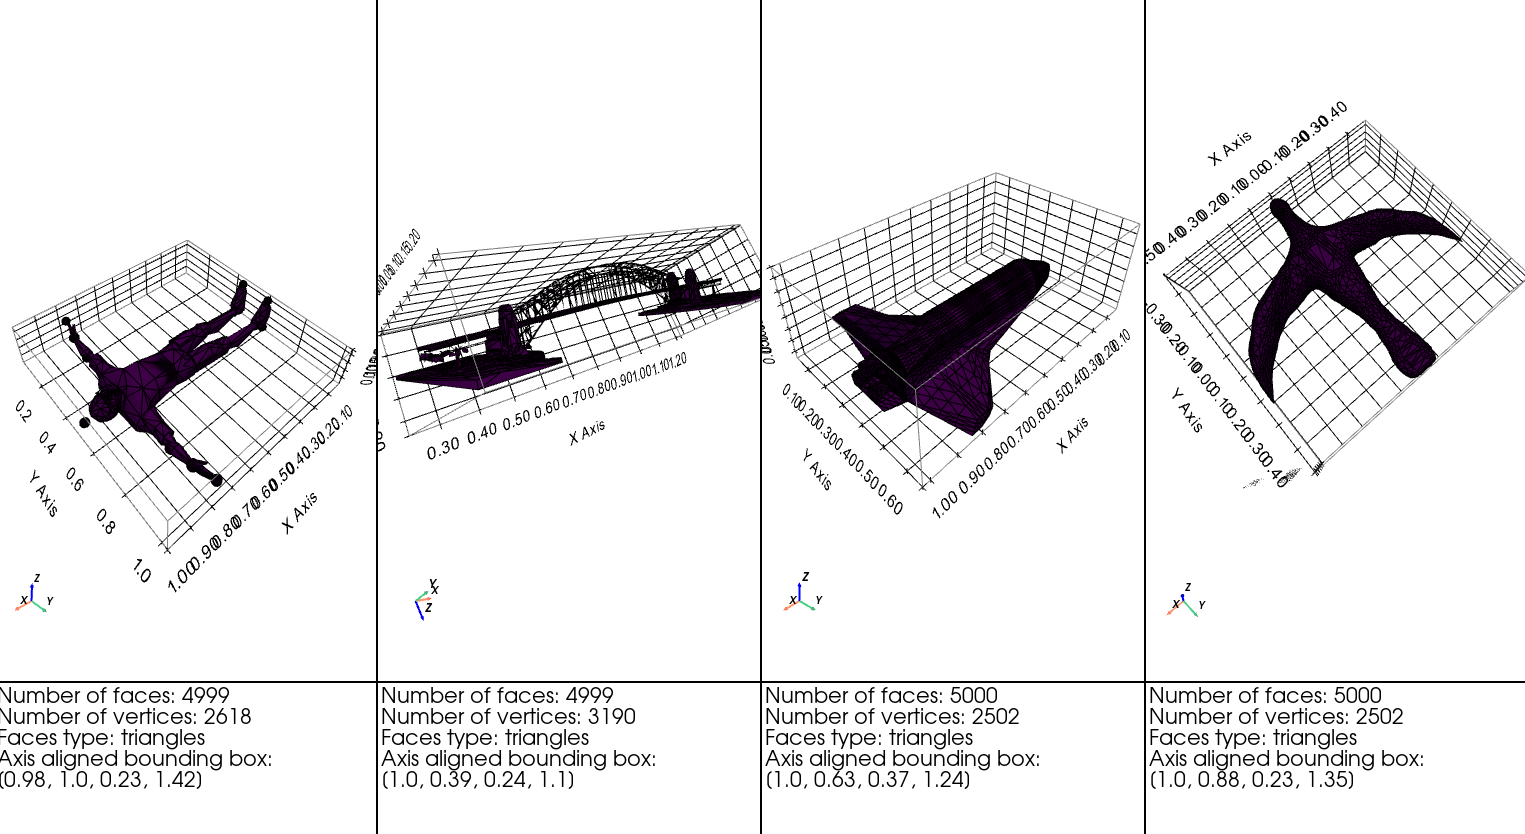
\includegraphics[width=\textwidth]{assets/queries/human_ann/output.png}
        \caption{Query output; Respective distances: 0.0181, 0.0189, 0.0222, 0.0310}
        \label{fig:query-output-ann-3}
    \end{subfigure}
    \hfill
    
    \caption{Example of the query response using ANN}
    \label{fig:query-response-example-ann}
\end{figure}

\begin{figure}[H]
    \centering
    \begin{subfigure}[b]{0.3\textwidth}
        \includegraphics[width=\textwidth]{assets/queries/ann_good/input.png}
        \caption{Query input \newline}
    \end{subfigure}
    \hfill
    \begin{subfigure}[b]{0.65\textwidth}
        \includegraphics[width=\textwidth]{assets/queries/ann_good/output_ann.png}
        \caption{Query output with ANN; \newline Respective distances: 0.0242, 0.0245, 0.0428, 0.0434}
    \end{subfigure}
    \hfill
    
    \begin{subfigure}[b]{0.3\textwidth}
        \includegraphics[width=\textwidth]{assets/queries/ann_good/input.png}
        \caption{Query input \newline}
    \end{subfigure}
    \hfill
    \begin{subfigure}[b]{0.65\textwidth}
        \includegraphics[width=\textwidth]{assets/queries/ann_good/output_knn.png}
        \caption{Query output with KNN;  Respective distances: \newline $10.384\cdot10^{-5}, 10.416\cdot10^{-5}, 10.713\cdot10^{-5}, 10.783\cdot10^{-5}$}
    \end{subfigure}
    \caption{Good example of the query response using ANN vs KNN (with tuned distance functions)}
    \label{fig:query-response-example-ann-good}
\end{figure}

\subsection{Dimensionality reduction}\label{subsec:dimensionality-reduction}
When making a query, the complexity when using a KNN is $O(N \cdot d)$, where $N$ is the number of shapes in the database, and $d$ is the length of their feature vectors.
Dimensionality reduction (DR) techniques aim to reduce the length of $d$, while still preserving as much of the discriminative information as possible.
This would result in smaller - and therefore easier to process, feature vectors, which will reduce the complexity of the querying operation.
While one could design a system which uses the reduced feature vectors for querying, we chose not to explore this approach, considering our ANN approach sufficient.
Instead, we use the technique to visualize the spatial relations of shapes in the database relative to each other.

Consider a feature vector reduction to a size of $2$ across our database.
The reduced vectors can then be plotted in a simple $2D$ plot, where the distance between points represents the difference between different shapes.
The result is shown in Figure (\ref{fig:feature-vectors-2D}).

\paragraph{t-SNE}
To perform the DR, we use an algorithm called t-distributed stochastic neighbour embedding (t-SNE) (see \cite{van2008visualizing} for details).
The algorithm consists of two main stages.
First, a probability distribution over pairs of high-dimensional feature vectors is computed, where similar vectors are assigned a higher probability, while dissimilar ones are assigned a lower one.
In assigning these probabilities, the algorithm uses Gaussian distributions, where the standard deviation is a user-given parameter called $perplexity$.
This parameter indirectly describes the radius of the $n$-dimensional ball centred at a point of the $n$-dimensional space (i.e.\ a feature vector), for which we assign probabilities.
Informally, assigning bigger values for perplexity is useful in sparse data spaces, whilst smaller values are useful in spaces where data is dense.
After the probability distribution for the high-dimensional space is created, a probability distribution is created over the points in the low-dimensional space (i.e.\ 2D) by using a form of $T$-distribution.
To find the new locations in the low-dimension space, the algorithm minimizes the Kullback–Leibler divergence (KL divergence) between the two distributions.

\subsubsection{Results}
Figure \ref{fig:feature-vectors-2D} presents a 2D visualization of our feature vectors with different values for the $perplexity$ parameter.
The technique produces informative results, however a limitation of the resulting is that, due to the fact we have $20$ shape classes, the colours of points can be close and therefore difficult to distinguish.
Also note that the colors of classes are randomly assigned on computation and as a result do not match between the two figures.
Still, there are clear clusters created and there are consistent patterns between Figures \ref{fig:feature-vectors-2D-perplexity-20} and \ref{fig:feature-vectors-2D-perplexity-40}.


The \textit{Mech} and \textit{Plant} classes result in very good clusters in both cases.
Another indication that the technique works well is the fact that clusters from not only within, but also between classes with similar features.
For instance, the \textit{Airplane} and \textit{Bird} classes - which we would expect to have similar features (i.e.\ a large flat area in the wings of both an airplane and a bird).

Still, the results are not perfect.
Notice how in both Figures \ref{fig:feature-vectors-2D-perplexity-20} and \ref{fig:feature-vectors-2D-perplexity-40}, there are some classes (e.g. \textit{vehicle}) tend to not form a cluster.
The feature vectors are rather spread out along the 2D space.
The reason for this is that, in these classes we have shapes that perceptually might be from the same class for a user, but do not share common features.
For instance, the \textit{vehicle} class contains cars, starships, ships, airplanes, tanks, and more.
Conceptually, all of the above are vehicles, but they have very divergent features.

\begin{figure}[H]
    \centering
    \begin{subfigure}[b]{0.55\textwidth}
         \includegraphics[width=\textwidth]{assets/evaluation_results/tsne_20.png}     
        \caption{$perplexity$=20}
        \label{fig:feature-vectors-2D-perplexity-20}
    \end{subfigure}
    \hfill
    \begin{subfigure}[b]{0.55\textwidth}
         \includegraphics[width=\textwidth]{assets/evaluation_results/tsne_40.png}
         \caption{$perplexity$=40}
         \label{fig:feature-vectors-2D-perplexity-40}
    \end{subfigure}    
    \caption{Feature vectors in 2D}
    \label{fig:feature-vectors-2D}
\end{figure}


\section{Retrieval System}
\label{section:retrieval-system}
In this section, we describe the interface with which a user can interact with our retrieval system.
Figure \ref{fig:gui-overview-app} shows the window that is opened to the user when the application is launched.
The user can select a folder with 3D shapes (the system will show only the files that have the extension \verb!".ply"!),
as shown in Figure \ref{fig:gui-overview-file-browser}.
To retrieve similar shapes, the user selects what shape they want to query on, and after clicking, a preview 
of the 3D shape is opened.
After closing the preview window, a query is performed when the \textbf{Retrieve similar shapes} button is selected.
The system returns a list of shapes according to the query, and a preview of 1--5 retrieved shapes is displayed.
The user also has the ability to use the system for retrieving all the shapes within a distance range in both default
and advanced modes.

If the query shape is present in our database, the system will find it internally with a distance of 0 - since it
is most similar to itself.
We don't consider this to be desirable for an end user, so the query shape is not returned as part of the results.
After closing the preview, the user can see the retrieved shapes' filenames, as well as the distance between each 
retrieved shape and the query.
Clicking on a shape from the retrieved list opens a 3D preview window with that shape. 

By default, the system uses a pre-computed index on the features database.
This index is constructed with a technique called Approximate Nearest Neighbours (ANN), which is discussed in detail 
in Section \ref{section:scalability}.
\begin{figure}[H]
    \centering
    \begin{subfigure}[b]{0.45\textwidth} 
        \includegraphics[width = \textwidth]{assets/GUI/retrieval_ann_example.png}
        \caption{System overview}
        \label{fig:gui-overview-app}
    \end{subfigure}
    \hfill
    \begin{subfigure}[b]{0.45\textwidth} 
        \includegraphics[width = \textwidth]{assets/GUI/folder_browser.png}
        \caption{Browsing shapes folders}
        \label{fig:gui-overview-file-browser}
    \end{subfigure}
    
    \caption{Multimedia retrieval system overview}
    \label{fig:gui-overview}
\end{figure}

\subsection{Advanced mode}
Optionally, the user can enter an advanced query mode by checking the\textbf{Advanced search} checkbox.
This allows the user to tune the distance functions, change the weights of certain features, and more.
Figure \ref{fig:gui-advanced-knn} shows the options which are available to the user when in advanced mode.

A set of new fields are displayed, in which the user can indicate how to weigh different parts of the feature
vector and which distance function they would prefer to use.
By default, the scalar distance function is the cosine distance, and the distance function for the histograms is the
Earth Mover's Distance (EMD).
The scalar distance functions are weighted in a 3:1 ratio to the histogram distance function.

\begin{figure}[H]
    \centering
    \begin{subfigure}[b]{0.45\textwidth} 
        \includegraphics[width = \textwidth]{assets/GUI/retrieval_knn_example.png}
        \caption{Advanced retrieval indicating $k$}
        \label{fig:gui-advanced-knn}
    \end{subfigure}
    \hfill
    \begin{subfigure}[b]{0.45\textwidth} 
        \includegraphics[width = \textwidth]{assets/GUI/retrieval_threshold_based.png}
        \caption{Advanced threshold-based retrieval}
        \label{fig:gui-advanced-threshold-based}
    \end{subfigure}
    \hfill
    
    \caption{Advanced retrieval}
    \label{fig:gui-advanced}
\end{figure}

\section{Evaluation}
\label{section:evaluation}
Evaluating a retrieval system is complex because we need to come up with a distance to compare how far is one result from another.
However, if we had such a perfect distance that tells us perfectly how similar an object is to another we would have included it in our system.
Notice that we can not use our own distance functions as evaluation metrics because in this case, the evaluation is not fair.

In order to overcome this problem we need to use in our evaluation metrics some information the system does not know about.
Luckily we have such information in the class labels of the shapes.
We must still note that, these class labels are not very detailed and each class can contain models that differ significantly, such as the \textit{Vehicle} class.
Still, in lieu of a better alternative, we consider the class labels the ground truth for our system. 
This allows us to use several metrics from machine learning for the evaluation of our retrieval results.

To visualize the process, consider the case in which the user makes a query with a shape of the \textit{Airplane} class and expects $k=1$ items to be returned.
A result is correct (True Positive ($TP$)) when a shape that is also of the \textit{Airplane} class is returned.
On the other hand, if a shape of any other class is returned, the result is incorrect (False Positive ($FP$)).
We compute the number of $TP$, $TN$, $FP$ and $FN$ results (see Table \ref{tab:tp-tn-fp-fn}) for our multi-class problem by means of a confusion matrix.

Extending this beyond $k=1$, the approach is to take the user-given shape and to create $k$ pairs of ground truth and predicted labels.

\begin{table}[ht]
    \centering
    \begin{tabular}{c|c|c|c}
         \multicolumn{2}{c|}{} & \multicolumn{2}{c}{Predicted class} \\
        \cline{3-4}
         \multicolumn{2}{c|}{} & 1 & 0 \\
        \hline
        \multirow{2}{*}{True class} & 1 & $TP$ (true positive)  & $FP$ (false positive) \\
        \cline{2-4}
        & 0 & $FN$ (false negative) & $TN$ (true negative) \\
    \end{tabular}
    \caption{Results notations}
    \label{tab:tp-tn-fp-fn}
\end{table}

After computing the confusion matrix we use a set of classical evaluation metrics from the machine learning field as described in Table \ref{tab:evaluation-metrics}.
Each metric aims to describe the system's performance from a different perspective (see Description column of Table \ref{tab:evaluation-metrics}).

\begin{table}[ht]
    \centering
    \resizebox{\textwidth}{!}{
        \begin{tabular}{c|c|c}
            Name & Formula & Description \\
            \hline
            Accuracy & $\frac{TP}{TP + FP + FN + TN}$ & The ratio of total correct predictions\\
            \hline
            \multirow{2}{*}{Precision} & \multirow{2}{*}{$\frac{TP_i}{TP_i + FP_i}$} & The ratio of the number of correct predictions within \\
            &  & a class to the number of class members\\
            \hline
            \multirow{2}{*}{Recall} & \multirow{2}{*}{$\frac{TP_i}{TP_i + FN_i}$} & The ratio of the number of correct predictions within \\
            & & a class to the total number of predictions assigned to class\\
            \hline
            \multirow{2}{*}{F1 score} &\multirow{2}{*}{$2 \cdot \frac{Precision_i \cdot Recall_i}{Precision_i + Recall_i}$} & Combines the precision and recall of a classifier \\
            & & into a single metric by taking their harmonic mean \\
            \hline
            \multirow{2}{*}{True Positive rate} & \multirow{2}{*}{$\frac{TP_i}{TP_i + FN_i}$} & The probability that an actual positive label \\
            & & will be predicted as positive\\
            \hline
            \multirow{2}{*}{False Positive rate} & \multirow{2}{*}{$\frac{FP_i}{FP_i + TN_i}$} &  The probability of wrongly predicting \\
            & & the label of a negative class\\
        \end{tabular}
    }
    \caption{Notations for the evaluation metrics}
    \label{tab:evaluation-metrics}
\end{table}

\paragraph{Receiver Operating Characteristic (ROC) curve}
We use an ROC curve to measure the performance of our system at different query sizes. \footnote{We direct readers without a background understanding of ROC curves to \cite{fawcett2006introduction}.}  % make a note below page
The \textbf{True Positive Rate} and \textbf{False Positive Rate} of the system are used to compute it as follows.
For each of the $20$ classes in our system, we consider one as the positive class and all of the other classes as negative ones (i.e.\ a one-vs-all approach).
We consider values of the query size $k$ from $1$ to $5$ and for each one, compute the True Positive and False Positive rates.
This process gives 5 points of the ROC curve, which we interpolate to give an approximation of the ROC curve for all classes.

There is a detail to note in our computation of the ROC curve in the cases where $k>1$.
We had to decide on what are considered a $TP$ and $FP$ result.
If a user requests $5$ shapes in their query, is $1$ correct one enough to consider the result successful;
conversely, if $1$ of the shapes returned is incorrect, but $4$ are, should the result be considered wrong in its entirety?
In our evaluation, we consider both a strict and a relaxed definition of the above.
The relaxed definition is, in cases where $k>1$, to consider a result correct if at least $k-1$ of the returned shapes are of the same class as the query shape.
While a compromise, we consider this to be the more informative metric as it is more consistent with what a user would consider satisfactory, at least at the sizes of $k$ (i.e.\ $<=5$) which we are interested in.

\subsection{Results and Discussion}
Table \ref{tab:accuracy} presents overall accuracy figures for our system at several query sizes.
Notice how the $KNN$ approach achieves a better accuracy overall than the faster $ANN$ approach.
As expected, the accuracy decreases as the query size increases.
 
\begin{table}[ht]
    \centering
    \begin{tabular}{c|c|c}
        \textbf{k} & \textbf{KNN} & \textbf{ANN} \\
        \hline
        1 & \textbf{62.10} & 60.29\\
        2 & \textbf{58.75} & 58.21\\
        3 & \textbf{55.70} & 52.73\\
        4 & \textbf{52.47} & 48.87\\
        5 & \textbf{50.26} & 44.90\\
    \end{tabular}
    \caption{KNN vs ANN in terms of accuracy}
    \label{tab:accuracy}
\end{table}

We compute the \textbf{Precision}, \textbf{Recall}, and \textbf{F1 score} for all classes at query sizes ($k \in  \{1, 3, 5\}$) using the relaxed evaluation condition.
Figures \ref{fig:knn-confusion-matrix-results} and \ref{fig:ann-confusion-matrix-results} show the confusion matrices for each query size.
Tables \ref{tab:precision-recall-f1-k-1}, \ref{tab:precision-recall-f1-k-3} and \ref{tab:precision-recall-f1-k-5} present the values of the above metrics for each class for both the $KNN$ and $ANN$ approaches.

Notice that for some classes we have higher values for all the metrics of interest and for other classes these values are quite low.
That is, our system deals better with discriminating against certain classes and performs poorly in discriminating against other certain classes.
This makes sense given that some class labels are more informative about the shape than others (recall the vehicle class contains cars, starships, ships, airplanes, tanks, and more).

The values for the \textbf{Precision} range between $27$ and $100$ and for \textbf{Recall} range between $19$ and $100$.
Notice inverse relationship between the average values of these metrics and $k$.
Moreover, observe again how the $KNN$ approach overall performs better than $ANN$.

\begin{table}[H]
    \centering
    \begin{tabular}{c|c|c|c|c|c|c}
         & \multicolumn{3}{c|}{KNN} & \multicolumn{3}{c}{ANN} \\
        \hline
        Class & Precision & Recall & F1 score & Precision & Recall & F1 score \\
        \hline
        plant & 71.43 & 68.72 & 70.05 & 80.28 & 76.05 & 78.11 \\ 
        furniture & 59.78 & 59.03 & 59.4 & 69.72 & 69.13 & 69.43 \\ 
        household & 57.77 & 39.43 & 46.87 & 67.96 & 21.79 & 33.0 \\ 
        vehicle & 62.38 & 44.69 & 52.07 & 68.16 & 32.99 & 44.46 \\ 
        building & 36.36 & 59.24 & 45.07 & 69.57 & 58.47 & 63.54 \\ 
        animal & 51.06 & 62.9 & 56.37 & 53.79 & 35.49 & 42.76 \\ 
        miscellaneous & 38.26 & 54.45 & 44.94 & 58.1 & 46.73 & 51.8 \\ 
        Bust & 42.86 & 45.0 & 43.9 & 41.67 & 54.64 & 47.28 \\ 
        Hand & 47.37 & 45.0 & 46.15 & 50.0 & 26.85 & 34.94 \\ 
        Bird & 68.75 & 55.0 & 61.11 & 38.71 & 72.14 & 50.38 \\ 
        Ant & 60.71 & 85.0 & 70.83 & 33.33 & 30.24 & 31.71 \\ 
        Table & 84.62 & 55.0 & 66.67 & 55.17 & 97.06 & 70.35 \\ 
        FourLeg & 38.89 & 35.0 & 36.84 & 52.38 & 65.98 & 58.4 \\ 
        Octopus & 47.06 & 40.0 & 43.24 & \textbf{100.0} & 36.23 & 53.19 \\ 
        Cup & 95.0 & \textbf{95.0} & \textbf{95.0} & 73.08 & 97.94 & 83.7 \\ 
        Airplane & 94.12 & 80.0 & 86.49 & 42.86 & 80.77 & 56.0 \\ 
        Human & 75.0 & 60.0 & 66.67 & 46.67 & 44.19 & 45.4 \\ 
        Plier & 95.0 & \textbf{95.0} & \textbf{95.0} & 63.64 & 85.09 & 72.82 \\ 
        Teddy & 63.64 & 70.0 & 66.67 & 79.17 & 99.52 & 88.18 \\ 
        Bearing & \textbf{100.0} & 86.05 & 92.5 & 47.06 & 83.8 & 60.27 \\ 
        Fish & 50.0 & 75.0 & 60.0 & 61.29 & 99.12 & 75.75 \\ 
        Chair & 71.43 & 75.0 & 73.17 & 95.24 & \textbf{100.0} & \textbf{97.56} \\ 
        Vase & 40.0 & 40.0 & 40.0 & 62.5 & 78.1 & 69.43 \\ 
        Armadillo & 31.82 & 35.0 & 33.33 & 66.67 & 68.41 & 67.53 \\ 
        Glasses & 90.48 & \textbf{95.0} & 92.68 & 69.23 & 64.16 & 66.6 \\ 
        Mech & 75.0 & 78.11 & 76.52 & 60.0 & 53.13 & 56.36 \\ 
        \hline
        \textbf{Average} & 63.41 & 62.79 & 62.37 & 61.78 & 64.54 & 60.34\\
    \end{tabular}
    \caption{KNN vs ANN in terms of Precision, Recall and F1 score for k=1}
    \label{tab:precision-recall-f1-k-1}
\end{table}

\begin{table}[H]
    \centering
    \begin{tabular}{c|c|c|c|c|c|c}
         & \multicolumn{3}{c|}{KNN} & \multicolumn{3}{c}{ANN} \\
        \hline
        Class & Precision & Recall & F1 score & Precision & Recall & F1 score \\
        \hline
        plant & 67.02 & 68.05 & 67.53 & 62.44 & 60.63 & 61.52 \\ 
        furniture & 53.98 & 55.62 & 54.79 & 49.06 & 48.47 & 48.76 \\
        household & 53.78 & 32.05 & 40.16 & 51.06 & 17.59 & 26.17 \\ 
        vehicle & 53.85 & 39.45 & 45.54 & 53.56 & 26.31 & 35.29 \\ 
        building & 27.41 & 49.14 & 35.19 & 46.15 & 51.54 & 48.7 \\ 
        animal & 45.68 & 61.46 & 52.4 & 48.1 & 24.38 & 32.36 \\ 
        miscellaneous & 33.66 & 42.82 & 37.7 & 50.38 & 36.61 & 42.4 \\ 
        Bust & 51.61 & 53.33 & 52.46 & 54.29 & 63.97 & 58.73 \\ 
        Hand & 39.66 & 38.33 & 38.98 & 28.17 & 38.05 & 32.37 \\ 
        Bird & 58.18 & 53.33 & 55.65 & 32.47 & 48.73 & 38.97 \\ 
        Ant & 51.9 & 68.33 & 58.99 & 42.37 & 46.21 & 44.21 \\ 
        Table & 74.36 & 50.17 & 59.91 & 51.06 & 71.32 & 59.52 \\ 
        FourLeg & 41.82 & 38.33 & 40.0 & 40.28 & 56.23 & 46.94 \\ 
        Octopus & 33.33 & 21.67 & 26.26 & 38.1 & 28.65 & 32.71 \\ 
        Cup & \textbf{91.38} & 88.33 & \textbf{89.83} & 59.74 & \textbf{91.71} & 72.35 \\ 
        Airplane & 71.83 & 85.0 & 77.86 & 45.07 & 68.98 & 54.52 \\ 
        Human & 40.62 & 43.33 & 41.94 & 40.38 & 42.83 & 41.57 \\ 
        Plier & 90.74 & 81.67 & 85.96 & 60.0 & 87.96 & 71.34 \\ 
        Teddy & 48.28 & 70.0 & 57.14 & 74.63 & 91.63 & \textbf{82.26} \\ 
        Bearing & 84.21 & 61.28 & 70.94 & 53.03 & 70.82 & 60.65 \\ 
        Fish & 46.34 & 63.33 & 53.52 & 62.86 & 78.78 & 69.92 \\ 
        Chair & 64.41 & 63.33 & 63.87 & 71.43 & 91.63 & 80.28 \\ 
        Vase & 46.0 & 38.33 & 41.82 & 66.67 & 66.81 & 66.74 \\ 
        Armadillo & 38.33 & 38.33 & 38.33 & 61.76 & 75.62 & 67.99 \\ 
        Glasses & 90.91 & \textbf{84.45} & 87.56 & 46.55 & 66.69 & 54.83 \\ 
        Mech & 70.97 & 76.44 & 73.6 & \textbf{82.14} & 76.67 & 79.31 \\
        \hline
        \textbf{Average} & 56.55 & 56.38 & 55.69 & 52.76 & 58.8 & 54.25\\
    \end{tabular}
    \caption{KNN vs ANN in terms of Precision, Recall and F1 score for k=3}
    \label{tab:precision-recall-f1-k-3}
\end{table}

\begin{table}[H]
    \centering
    \begin{tabular}{c|c|c|c|c|c|c}
         & \multicolumn{3}{c|}{KNN} & \multicolumn{3}{c}{ANN} \\
        \hline
        Class & Precision & Recall & F1 score & Precision & Recall & F1 score \\
        \hline
        plant & 65.68 & 62.86 & 64.24 & 56.39 & 48.27 & 52.01 \\ 
        furniture & 48.64 & 49.16 & 48.9 & 37.52 & 32.63 & 34.91 \\ 
        household & 52.74 & 29.21 & 37.6 & 40.82 & 12.8 & 19.49 \\ 
        vehicle & 49.7 & 35.96 & 41.73 & 47.26 & 20.02 & 28.12 \\ 
        building & 25.21 & 47.8 & 33.01 & 37.96 & 40.78 & 39.32 \\ 
        animal & 41.75 & 57.6 & 48.41 & 41.46 & 18.01 & 25.11 \\ 
        miscellaneous & 32.37 & 39.27 & 35.48 & 40.42 & 30.65 & 34.86 \\ 
        Bust & 49.5 & 50.0 & 49.75 & 42.61 & 52.98 & 47.23 \\ 
        Hand & 37.89 & 36.0 & 36.92 & 23.97 & 33.97 & 28.1 \\ 
        Bird & 45.0 & 45.0 & 45.0 & 25.0 & 37.36 & 29.96 \\ 
        Ant & 43.51 & 57.0 & 49.35 & 37.04 & 45.98 & 41.03 \\ 
        Table & 65.71 & 48.21 & 55.62 & 34.44 & 61.73 & 44.22 \\ 
        FourLeg & 37.23 & 35.0 & 36.08 & 34.45 & 47.21 & 39.84 \\ 
        Octopus & 27.94 & 19.0 & 22.62 & 34.88 & 31.8 & 33.27 \\ 
        Cup & \textbf{89.69} & \textbf{87.0} & \textbf{88.32} & 49.18 & 84.36 & 62.14 \\ 
        Airplane & 69.03 & 78.0 & 73.24 & 42.48 & 61.66 & 50.3 \\ 
        Human & 33.65 & 35.0 & 34.31 & 29.73 & 41.8 & 34.75 \\ 
        Plier & 75.73 & 78.0 & 76.85 & 54.41 & \textbf{87.95} & 67.23 \\ 
        Teddy & 44.44 & 72.0 & 54.96 & 70.25 & 87.38 & \textbf{77.88} \\ 
        Bearing & 74.51 & 43.64 & 55.04 & 43.0 & 56.51 & 48.84 \\ 
        Fish & 42.22 & 57.0 & 48.51 & 59.13 & 74.4 & 65.89 \\ 
        Chair & 56.7 & 55.0 & 55.84 & 60.95 & 83.38 & 70.42 \\ 
        Vase & 35.79 & 34.0 & 34.87 & 60.98 & 55.77 & 58.26 \\ 
        Armadillo & 31.73 & 33.0 & 32.35 & 56.19 & 66.63 & 60.96 \\ 
        Glasses & 87.34 & 70.19 & 77.83 & 33.01 & 60.68 & 42.76 \\ 
        Mech & 71.58 & 70.27 & 70.92 & \textbf{71.82} & 79.0 & 75.24 \\ 
        \hline
        \textbf{Average} & 51.36 & 50.97 & 50.3 & 44.82 & 52.06 & 46.62\\
    \end{tabular}
    \caption{KNN vs ANN in terms of Precision, Recall and F1 score for k=5}
    \label{tab:precision-recall-f1-k-5}
\end{table}

Figures \ref{fig:knn-roc-curve-results} and \ref{fig:ann-roc-curve-results} present the computed ROC curves for $KNN$ and $ANN$ approaches respectively.
Notice how the ROC curves for certain classes have a higher area under the curve than for other classes for both approaches.
Using the relaxed definition of the correct prediction observe how the area under the curve for all the classes increases considerably.
This means that, even though for certain classes the results are not exclusively of the same class as the query shape, the returned shapes are still overwhelmingly of the correct class.
Figure \ref{fig:knn-vs-ann-human-roc-curve-results} presents two ROC curves for the Human class for the $KNN$ and $ANN$ approaches respectively.
With both the strict and relaxed versions, the area under the curve for the $KNN$ is bigger than for $ANN$, which confirms once again that the $KNN$ approach performs slightly better than the faster $ANN$ one.

\section{Conclusion}
\label{section:conclusions}
This report describes the implementation of a 3D shape retrieval system based on a set of discriminative features.
We describe how a 3D shape dataset should be preprocessed in order to extract good features which are consistent across a variety of shapes.
For each step of the preprocessing, we demonstrate the correctness of the implementation.
An extensive analysis, involving both theoretical shapes and ones from the dataset, is done on the computed features in order to evaluate the correctness of our implementation and ensure the features' discriminative power.
We present and evaluate several functions for computing a distance between shapes based on their features.

Our system allows for the choice between using a precomputed index for searching quickly, useful for large datasets, or a custom combination of weights and distance functions, which allow for the possibility of more accurate results at the cost of the speed.
On the one hand, the precomputed index approach gives results an order of magnitude faster, but on the other hand, the results are less accurate.
Since the priorities differ for different applications, in order to achieve a system that is flexible, we allow the user to make this decision, even though by default our system aims for speed and ease of use, and thus uses the precomputed index.

Our quantitative evaluation shows that overall the system does not perform ideally, but excels at certain, more limited, classes of objects.
Ideally, we would have liked to evaluate the system with more fine-grained ground truth labels for our data, but that was not possible with the dataset we chose.
Of course, the decision about how well the system performs depends on the domain and use-case, and should be decided as the system would be integrated into a larger application.
Used on its own, the system performs relatively well, however, there is room for improvement.
For example, further evaluation could be done to determine the ideal combination of feature weights and distance functions.
Additionally, future work could examine more features (e.g.\ a histogram of the local distribution of curvatures of a shape) to achieve greater discriminative power, as well as evaluate the system on a different dataset with more classes.
A further investigation in the direction of dimensionality reduction with t-SNE is also possible, for example to use icons as representations of certain clusters \& regions of the image, instead of a color for an entire class.

\pagebreak
\bibliographystyle{alpha}
\bibliography{sample}

\pagebreak
\appendix
\section{Appendix 1}
\hrule
\begin{table}[ht]
\centering
\begin{tabular}{|l|}
\hline
"data/PRINCETON/train/plant/m1063.ply",         \\ \hline
"data/PRINCETON/train/plant/m1030.ply",         \\ \hline
"data/PRINCETON/train/animal/m171.ply",         \\ \hline
"data/PRINCETON/train/animal/m8.ply",           \\ \hline
"data/PRINCETON/train/animal/m74.ply",          \\ \hline
"data/PRINCETON/train/animal/m244.ply",         \\ \hline
"data/PRINCETON/train/building/m388.ply",       \\ \hline
"data/PRINCETON/train/building/m407.ply",       \\ \hline
"data/PRINCETON/train/building/m415.ply",       \\ \hline
"data/PRINCETON/train/furniture/m926.ply",      \\ \hline
"data/PRINCETON/train/furniture/m925.ply",      \\ \hline
"data/PRINCETON/train/furniture/m924.ply",      \\ \hline
"data/PRINCETON/train/furniture/m929.ply",      \\ \hline
"data/PRINCETON/train/furniture/m892.ply",      \\ \hline
"data/PRINCETON/train/furniture/m840.ply",      \\ \hline
"data/PRINCETON/train/household/m538.ply",      \\ \hline
"data/PRINCETON/train/household/m570.ply",      \\ \hline
"data/PRINCETON/train/household/m611.ply",      \\ \hline
"data/PRINCETON/train/household/m612.ply",      \\ \hline
"data/PRINCETON/train/household/m690.ply",      \\ \hline
"data/PRINCETON/train/household/m754.ply",      \\ \hline
"data/PRINCETON/train/household/m758.ply",      \\ \hline
"data/PRINCETON/train/household/m1761.ply",     \\ \hline
"data/PRINCETON/train/miscellaneous/m1783.ply", \\ \hline
"data/PRINCETON/train/miscellaneous/m1625.ply", \\ \hline
"data/PRINCETON/train/miscellaneous/m1620.ply", \\ \hline
"data/PRINCETON/train/vehicle/m1399.ply",       \\ \hline
"data/PRINCETON/train/vehicle/m1185.ply",       \\ \hline
"data/PRINCETON/train/vehicle/m1406.ply",       \\ \hline
"data/PRINCETON/train/vehicle/m1300.ply",       \\ \hline
"data/PRINCETON/train/vehicle/m1189.ply",       \\ \hline
"data/PRINCETON/train/vehicle/m1225.ply",       \\ \hline
"data/PRINCETON/train/vehicle/m1221.ply",       \\ \hline
"data/PRINCETON/train/vehicle/m1237.ply",       \\ \hline
"data/PRINCETON/train/vehicle/m1520.ply",       \\ \hline
"data/PRINCETON/train/vehicle/m1197.ply",       \\ \hline
"data/PRINCETON/train/vehicle/m1333.ply",       \\ \hline
"data/PRINCETON/train/vehicle/m1335.ply",       \\ \hline
"data/PRINCETON/train/vehicle/m1233.ply",       \\ \hline
"data/PRINCETON/train/vehicle/m1450.ply",       \\ \hline
\end{tabular}
\caption{List of shapes which were removed from the database.}
\label{tab:my-table}
\end{table}

\begin{figure}[ht]
    \centering
    
    \begin{subfigure}[b]{0.4\textwidth}
        \includegraphics[width=\textwidth]{assets/visualisation/D1.png}
        \caption{D1}
        \label{fig:local_descriptor_visualisation_D1}
    \end{subfigure}
    \hfill
    \begin{subfigure}[b]{0.4\textwidth}
        \includegraphics[width=\textwidth]{assets/visualisation/D2.png}
        \caption{D2}
        \label{fig:local_descriptor_visualisation_D2}
    \end{subfigure}
    \hfill
    
    \begin{subfigure}[b]{0.4\textwidth}
        \includegraphics[width=\textwidth]{assets/visualisation/D3.png}
        \caption{D3}
        \label{fig:local_descriptor_visualisation_D3}
    \end{subfigure}
    \hfill
    \begin{subfigure}[b]{0.4\textwidth}
        \includegraphics[width=\textwidth]{assets/visualisation/D4.png}
        \caption{D4}
        \label{fig:local_descriptor_visualisation_D4}
    \end{subfigure}
    \hfill

    \begin{subfigure}[b]{0.4\textwidth}
        \includegraphics[width=\textwidth]{assets/visualisation/A3.png}
        \caption{A3}
        \label{fig:local_descriptor_visualisation_A3}
    \end{subfigure}
    \hfill
    
    \caption{Local descriptors visualisation}
    \label{fig:local_descriptor_visualisation}
\end{figure}

\begin{figure}[ht]
    \centering
    \begin{subfigure}[b]{0.23\textwidth}
        \includegraphics[width=\textwidth]{assets/feature_extraction/A3/Airplane.png}
        \caption{Airplane}
        \label{fig:features-statistics-A3-a}    
    \end{subfigure}
    \hfill
    \begin{subfigure}[b]{0.23\textwidth}
        \includegraphics[width=\textwidth]{assets/feature_extraction/A3/animal.png}
        \caption{animal}
        \label{fig:features-statistics-A3-b}    
    \end{subfigure}
    \hfill
    \begin{subfigure}[b]{0.23\textwidth}
        \includegraphics[width=\textwidth]{assets/feature_extraction/A3/Ant.png}
        \caption{Ant}
        \label{fig:features-statistics-A3-c}    
    \end{subfigure}
    \hfill    
    \begin{subfigure}[b]{0.23\textwidth}
        \includegraphics[width=\textwidth]{assets/feature_extraction/A3/Armadillo.png}
        \caption{Armadillo}
        \label{fig:features-statistics-A3-d}    
    \end{subfigure}
    \hfill
    
    \begin{subfigure}[b]{0.23\textwidth}
        \includegraphics[width=\textwidth]{assets/feature_extraction/A3/Bearing.png}
        \caption{Bearing}
        \label{fig:features-statistics-A3-e}    
    \end{subfigure}
    \hfill
    \begin{subfigure}[b]{0.23\textwidth}
        \includegraphics[width=\textwidth]{assets/feature_extraction/A3/Bird.png}
        \caption{Bird}
        \label{fig:features-statistics-A3-f}    
    \end{subfigure}
    \hfill
    \begin{subfigure}[b]{0.23\textwidth}
        \includegraphics[width=\textwidth]{assets/feature_extraction/A3/Bust.png}
        \caption{Bust}
        \label{fig:features-statistics-A3-g}    
    \end{subfigure}
    \hfill
    \begin{subfigure}[b]{0.23\textwidth}
        \includegraphics[width=\textwidth]{assets/feature_extraction/A3/building.png}
        \caption{Bird}
        \label{fig:features-statistics-A3-h}    
    \end{subfigure}
    \hfill

    
    \begin{subfigure}[b]{0.23\textwidth}
        \includegraphics[width=\textwidth]{assets/feature_extraction/A3/Chair.png}
        \caption{Chair}
        \label{fig:features-statistics-A3-i}    
    \end{subfigure}
    \hfill
    \begin{subfigure}[b]{0.23\textwidth}
        \includegraphics[width=\textwidth]{assets/feature_extraction/A3/Cup.png}
        \caption{Cup}
        \label{fig:features-statistics-A3-j}    
    \end{subfigure}
    \hfill
    \begin{subfigure}[b]{0.23\textwidth}
        \includegraphics[width=\textwidth]{assets/feature_extraction/A3/Fish.png}
        \caption{Fish}
        \label{fig:features-statistics-A3-k}    
    \end{subfigure}
    \hfill
    \begin{subfigure}[b]{0.23\textwidth}
        \includegraphics[width=\textwidth]{assets/feature_extraction/A3/FourLeg.png}
        \caption{Four Leg}
        \label{fig:features-statistics-A3-l}    
    \end{subfigure}
    \hfill

    \begin{subfigure}[b]{0.23\textwidth}
        \includegraphics[width=\textwidth]{assets/feature_extraction/A3/furniture.png}
        \caption{Furniture}
        \label{fig:features-statistics-A3-m}    
    \end{subfigure}
    \hfill
    \begin{subfigure}[b]{0.23\textwidth}
        \includegraphics[width=\textwidth]{assets/feature_extraction/A3/Glasses.png}
        \caption{Glasses}
        \label{fig:features-statistics-A3-n}    
    \end{subfigure}
    \hfill
    \begin{subfigure}[b]{0.23\textwidth}
        \includegraphics[width=\textwidth]{assets/feature_extraction/A3/Hand.png}
        \caption{Hand}
        \label{fig:features-statistics-A3-o}    
    \end{subfigure}
    \hfill
    \begin{subfigure}[b]{0.23\textwidth}
        \includegraphics[width=\textwidth]{assets/feature_extraction/A3/household.png}
        \caption{Household}
        \label{fig:features-statistics-A3-p}    
    \end{subfigure}
    \hfill

    \begin{subfigure}[b]{0.23\textwidth}
        \includegraphics[width=\textwidth]{assets/feature_extraction/A3/Human.png}
        \caption{Human}
        \label{fig:features-statistics-A3-q}    
    \end{subfigure}
    \hfill
    \begin{subfigure}[b]{0.23\textwidth}
        \includegraphics[width=\textwidth]{assets/feature_extraction/A3/Mech.png}
        \caption{Mech}
        \label{fig:features-statistics-A3-r}    
    \end{subfigure}
    \hfill
    \begin{subfigure}[b]{0.23\textwidth}
        \includegraphics[width=\textwidth]{assets/feature_extraction/A3/miscellaneous.png}
        \caption{Miscellaneous}
        \label{fig:features-statistics-A3-s}    
    \end{subfigure}
    \hfill
    \begin{subfigure}[b]{0.23\textwidth}
        \includegraphics[width=\textwidth]{assets/feature_extraction/A3/Octopus.png}
        \caption{Octopus}
        \label{fig:features-statistics-A3-t}    
    \end{subfigure}
    \hfill
    \caption{A3 signature for different classes}
    \label{fig:A3-signatures-1}
\end{figure}

\begin{figure}[ht]
    \centering
      \begin{subfigure}[b]{0.23\textwidth}
        \includegraphics[width=\textwidth]{assets/feature_extraction/A3/plant.png}
        \caption{Plant}
        \label{fig:features-statistics-A3-u}    
    \end{subfigure}
    \hfill
    \begin{subfigure}[b]{0.23\textwidth}
        \includegraphics[width=\textwidth]{assets/feature_extraction/A3/Plier.png}
        \caption{Plier}
        \label{fig:features-statistics-A3-v}    
    \end{subfigure}
    \hfill
    \begin{subfigure}[b]{0.23\textwidth}
        \includegraphics[width=\textwidth]{assets/feature_extraction/A3/Table.png}
        \caption{Table}
        \label{fig:features-statistics-A3-w}    
    \end{subfigure}
    \hfill
    \begin{subfigure}[b]{0.23\textwidth}
        \includegraphics[width=\textwidth]{assets/feature_extraction/A3/Teddy.png}
        \caption{Teddy bear}
        \label{fig:features-statistics-A3-x}    
    \end{subfigure}
    \hfill

    \begin{subfigure}[b]{0.23\textwidth}
        \includegraphics[width=\textwidth]{assets/feature_extraction/A3/Vase.png}
        \caption{Vase}
        \label{fig:features-statistics-A3-y}    
    \end{subfigure}
    \hfill
    \begin{subfigure}[b]{0.23\textwidth}
        \includegraphics[width=\textwidth]{assets/feature_extraction/A3/vehicle.png}
        \caption{Vehicle}
        \label{fig:features-statistics-A3-z}    
    \end{subfigure}
    \hfill
    
    \caption{A3 signatures for different classes}
    \label{fig:A3-signatures-2}
\end{figure}

\begin{figure}[t!p]
    \centering
    \begin{subfigure}[b]{0.23\textwidth}
        \includegraphics[width=\textwidth]{assets/feature_extraction/D1/Airplane.png}
        \caption{Airplane}
        \label{fig:features-statistics-D1-a}    
    \end{subfigure}
    \hfill
    \begin{subfigure}[b]{0.23\textwidth}
        \includegraphics[width=\textwidth]{assets/feature_extraction/D1/animal.png}
        \caption{animal}
        \label{fig:features-statistics-D1-b}    
    \end{subfigure}
    \hfill
    \begin{subfigure}[b]{0.23\textwidth}
        \includegraphics[width=\textwidth]{assets/feature_extraction/D1/Ant.png}
        \caption{Ant}
        \label{fig:features-statistics-D1-c}    
    \end{subfigure}
    \hfill    
    \begin{subfigure}[b]{0.23\textwidth}
        \includegraphics[width=\textwidth]{assets/feature_extraction/D1/Armadillo.png}
        \caption{Armadillo}
        \label{fig:features-statistics-D1-d}    
    \end{subfigure}
    \hfill
    
    \begin{subfigure}[b]{0.23\textwidth}
        \includegraphics[width=\textwidth]{assets/feature_extraction/D1/Bearing.png}
        \caption{Bearing}
        \label{fig:features-statistics-D1-e}    
    \end{subfigure}
    \hfill
    \begin{subfigure}[b]{0.23\textwidth}
        \includegraphics[width=\textwidth]{assets/feature_extraction/D1/Bird.png}
        \caption{Bird}
        \label{fig:features-statistics-D1-f}    
    \end{subfigure}
    \hfill
    \begin{subfigure}[b]{0.23\textwidth}
        \includegraphics[width=\textwidth]{assets/feature_extraction/D1/Bust.png}
        \caption{Bust}
        \label{fig:features-statistics-D1-g}    
    \end{subfigure}
    \hfill
    \begin{subfigure}[b]{0.23\textwidth}
        \includegraphics[width=\textwidth]{assets/feature_extraction/D1/building.png}
        \caption{Bird}
        \label{fig:features-statistics-D1-h}    
    \end{subfigure}
    \hfill

    
    \begin{subfigure}[b]{0.23\textwidth}
        \includegraphics[width=\textwidth]{assets/feature_extraction/D1/Chair.png}
        \caption{Chair}
        \label{fig:features-statistics-D1-i}    
    \end{subfigure}
    \hfill
    \begin{subfigure}[b]{0.23\textwidth}
        \includegraphics[width=\textwidth]{assets/feature_extraction/D1/Cup.png}
        \caption{Cup}
        \label{fig:features-statistics-D1-j}    
    \end{subfigure}
    \hfill
    \begin{subfigure}[b]{0.23\textwidth}
        \includegraphics[width=\textwidth]{assets/feature_extraction/D1/Fish.png}
        \caption{Fish}
        \label{fig:features-statistics-D1-k}    
    \end{subfigure}
    \hfill
    \begin{subfigure}[b]{0.23\textwidth}
        \includegraphics[width=\textwidth]{assets/feature_extraction/D1/FourLeg.png}
        \caption{Four Leg}
        \label{fig:features-statistics-D1-l}    
    \end{subfigure}
    \hfill

    \begin{subfigure}[b]{0.23\textwidth}
        \includegraphics[width=\textwidth]{assets/feature_extraction/D1/furniture.png}
        \caption{Furniture}
        \label{fig:features-statistics-D1-m}    
    \end{subfigure}
    \hfill
    \begin{subfigure}[b]{0.23\textwidth}
        \includegraphics[width=\textwidth]{assets/feature_extraction/D1/Glasses.png}
        \caption{Glasses}
        \label{fig:features-statistics-D1-n}    
    \end{subfigure}
    \hfill
    \begin{subfigure}[b]{0.23\textwidth}
        \includegraphics[width=\textwidth]{assets/feature_extraction/D1/Hand.png}
        \caption{Hand}
        \label{fig:features-statistics-D1-o}    
    \end{subfigure}
    \hfill
    \begin{subfigure}[b]{0.23\textwidth}
        \includegraphics[width=\textwidth]{assets/feature_extraction/D1/household.png}
        \caption{Household}
        \label{fig:features-statistics-D1-p}    
    \end{subfigure}
    \hfill

    \begin{subfigure}[b]{0.23\textwidth}
        \includegraphics[width=\textwidth]{assets/feature_extraction/D1/Human.png}
        \caption{Human}
        \label{fig:features-statistics-D1-q}    
    \end{subfigure}
    \hfill
    \begin{subfigure}[b]{0.23\textwidth}
        \includegraphics[width=\textwidth]{assets/feature_extraction/D1/Mech.png}
        \caption{Mech}
        \label{fig:features-statistics-D1-r}    
    \end{subfigure}
    \hfill
    \begin{subfigure}[b]{0.23\textwidth}
        \includegraphics[width=\textwidth]{assets/feature_extraction/D1/miscellaneous.png}
        \caption{Miscellaneous}
        \label{fig:features-statistics-D1-s}    
    \end{subfigure}
    \hfill
    \begin{subfigure}[b]{0.23\textwidth}
        \includegraphics[width=\textwidth]{assets/feature_extraction/D1/Octopus.png}
        \caption{Octopus}
        \label{fig:features-statistics-D1-t}    
    \end{subfigure}
    \hfill
    \caption{D1 signature for different classes}
    \label{fig:D1-signatures-1}
\end{figure}

\begin{figure}
    \centering
      \begin{subfigure}[b]{0.23\textwidth}
        \includegraphics[width=\textwidth]{assets/feature_extraction/D1/plant.png}
        \caption{Plant}
        \label{fig:features-statistics-D1-u}    
    \end{subfigure}
    \hfill
    \begin{subfigure}[b]{0.23\textwidth}
        \includegraphics[width=\textwidth]{assets/feature_extraction/D1/Plier.png}
        \caption{Plier}
        \label{fig:features-statistics-D1-v}    
    \end{subfigure}
    \hfill
    \begin{subfigure}[b]{0.23\textwidth}
        \includegraphics[width=\textwidth]{assets/feature_extraction/D1/Table.png}
        \caption{Table}
        \label{fig:features-statistics-D1-w}    
    \end{subfigure}
    \hfill
    \begin{subfigure}[b]{0.23\textwidth}
        \includegraphics[width=\textwidth]{assets/feature_extraction/D1/Teddy.png}
        \caption{Teddy bear}
        \label{fig:features-statistics-D1-x}    
    \end{subfigure}
    \hfill

    \begin{subfigure}[b]{0.23\textwidth}
        \includegraphics[width=\textwidth]{assets/feature_extraction/D1/Vase.png}
        \caption{Vase}
        \label{fig:features-statistics-D1-y}    
    \end{subfigure}
    \hfill
    \begin{subfigure}[b]{0.23\textwidth}
        \includegraphics[width=\textwidth]{assets/feature_extraction/D1/vehicle.png}
        \caption{Vehicle}
        \label{fig:features-statistics-D1-z}    
    \end{subfigure}
    \hfill
    
    \caption{D1 signatures for different classes}
    \label{fig:D1-signatures-2}
\end{figure}

\begin{figure}[t!p]
    \centering
    \begin{subfigure}[b]{0.23\textwidth}
        \includegraphics[width=\textwidth]{assets/feature_extraction/D2/Airplane.png}
        \caption{Airplane}
    \end{subfigure}
    \hfill
    \begin{subfigure}[b]{0.23\textwidth}
        \includegraphics[width=\textwidth]{assets/feature_extraction/D2/animal.png}
        \caption{animal}    
    \end{subfigure}
    \hfill
    \begin{subfigure}[b]{0.23\textwidth}
        \includegraphics[width=\textwidth]{assets/feature_extraction/D2/Ant.png}
        \caption{Ant}
    \end{subfigure}
    \hfill    
    \begin{subfigure}[b]{0.23\textwidth}
        \includegraphics[width=\textwidth]{assets/feature_extraction/D2/Armadillo.png}
        \caption{Armadillo}
    \end{subfigure}
    \hfill
    
    \begin{subfigure}[b]{0.23\textwidth}
        \includegraphics[width=\textwidth]{assets/feature_extraction/D2/Bearing.png}
        \caption{Bearing}
    \end{subfigure}
    \hfill
    \begin{subfigure}[b]{0.23\textwidth}
        \includegraphics[width=\textwidth]{assets/feature_extraction/D2/Bird.png}
        \caption{Bird}
    \end{subfigure}
    \hfill
    \begin{subfigure}[b]{0.23\textwidth}
        \includegraphics[width=\textwidth]{assets/feature_extraction/D2/Bust.png}
        \caption{Bust}
    \end{subfigure}
    \hfill
    \begin{subfigure}[b]{0.23\textwidth}
        \includegraphics[width=\textwidth]{assets/feature_extraction/D2/Bird.png}
        \caption{Bird}
        \label{fig:features-statistics-D2-h}    
    \end{subfigure}
    \hfill

    
    \begin{subfigure}[b]{0.23\textwidth}
        \includegraphics[width=\textwidth]{assets/feature_extraction/D2/Chair.png}
        \caption{Chair}
    \end{subfigure}
    \hfill
    \begin{subfigure}[b]{0.23\textwidth}
        \includegraphics[width=\textwidth]{assets/feature_extraction/D2/Cup.png}
        \caption{Cup}
    \end{subfigure}
    \hfill
    \begin{subfigure}[b]{0.23\textwidth}
        \includegraphics[width=\textwidth]{assets/feature_extraction/D2/Fish.png}
        \caption{Fish}
    \end{subfigure}
    \hfill
    \begin{subfigure}[b]{0.23\textwidth}
        \includegraphics[width=\textwidth]{assets/feature_extraction/D2/FourLeg.png}
        \caption{Four Leg}
    \end{subfigure}
    \hfill

    \begin{subfigure}[b]{0.23\textwidth}
        \includegraphics[width=\textwidth]{assets/feature_extraction/D2/furniture.png}
        \caption{Furniture}
    \end{subfigure}
    \hfill
    \begin{subfigure}[b]{0.23\textwidth}
        \includegraphics[width=\textwidth]{assets/feature_extraction/D2/Glasses.png}
        \caption{Glasses}
    \end{subfigure}
    \hfill
    \begin{subfigure}[b]{0.23\textwidth}
        \includegraphics[width=\textwidth]{assets/feature_extraction/D2/Hand.png}
        \caption{Hand}
    \end{subfigure}
    \hfill
    \begin{subfigure}[b]{0.23\textwidth}
        \includegraphics[width=\textwidth]{assets/feature_extraction/D2/household.png}
        \caption{Household}
    \end{subfigure}
    \hfill

    \begin{subfigure}[b]{0.23\textwidth}
        \includegraphics[width=\textwidth]{assets/feature_extraction/D2/Human.png}
        \caption{Human}
    \end{subfigure}
    \hfill
    \begin{subfigure}[b]{0.23\textwidth}
        \includegraphics[width=\textwidth]{assets/feature_extraction/D2/Mech.png}
        \caption{Mech}
    \end{subfigure}
    \hfill
    \begin{subfigure}[b]{0.23\textwidth}
        \includegraphics[width=\textwidth]{assets/feature_extraction/D2/miscellaneous.png}
        \caption{Miscellaneous}
    \end{subfigure}
    \hfill
    \begin{subfigure}[b]{0.23\textwidth}
        \includegraphics[width=\textwidth]{assets/feature_extraction/D2/Octopus.png}
        \caption{Octopus}
    \end{subfigure}
    \hfill
    \caption{D2 signature for different classes}
    \label{fig:D2-signatures-1}
\end{figure}

\begin{figure}
    \centering
      \begin{subfigure}[b]{0.23\textwidth}
        \includegraphics[width=\textwidth]{assets/feature_extraction/D2/plant.png}
        \caption{Plant}
    \end{subfigure}
    \hfill
    \begin{subfigure}[b]{0.23\textwidth}
        \includegraphics[width=\textwidth]{assets/feature_extraction/D2/Plier.png}
        \caption{Plier}
    \end{subfigure}
    \hfill
    \begin{subfigure}[b]{0.23\textwidth}
        \includegraphics[width=\textwidth]{assets/feature_extraction/D2/Table.png}
        \caption{Table}
    \end{subfigure}
    \hfill
    \begin{subfigure}[b]{0.23\textwidth}
        \includegraphics[width=\textwidth]{assets/feature_extraction/D2/Teddy.png}
        \caption{Teddy bear}
    \end{subfigure}
    \hfill

    \begin{subfigure}[b]{0.23\textwidth}
        \includegraphics[width=\textwidth]{assets/feature_extraction/D2/Vase.png}
        \caption{Vase}
    \end{subfigure}
    \hfill
    \begin{subfigure}[b]{0.23\textwidth}
        \includegraphics[width=\textwidth]{assets/feature_extraction/D2/vehicle.png}
        \caption{Vehicle}
    \end{subfigure}
    \hfill
    
    \caption{D2 signatures for different classes}
    \label{fig:D2-signatures-2}
\end{figure}

\begin{figure}[t!p]
    \centering
    \begin{subfigure}[b]{0.23\textwidth}
        \includegraphics[width=\textwidth]{assets/feature_extraction/D3/Airplane.png}
        \caption{Airplane}
    \end{subfigure}
    \hfill
    \begin{subfigure}[b]{0.23\textwidth}
        \includegraphics[width=\textwidth]{assets/feature_extraction/D3/animal.png}
        \caption{animal}    
    \end{subfigure}
    \hfill
    \begin{subfigure}[b]{0.23\textwidth}
        \includegraphics[width=\textwidth]{assets/feature_extraction/D3/Ant.png}
        \caption{Ant}
    \end{subfigure}
    \hfill    
    \begin{subfigure}[b]{0.23\textwidth}
        \includegraphics[width=\textwidth]{assets/feature_extraction/D3/Armadillo.png}
        \caption{Armadillo}
    \end{subfigure}
    \hfill
    
    \begin{subfigure}[b]{0.23\textwidth}
        \includegraphics[width=\textwidth]{assets/feature_extraction/D3/Bearing.png}
        \caption{Bearing}
    \end{subfigure}
    \hfill
    \begin{subfigure}[b]{0.23\textwidth}
        \includegraphics[width=\textwidth]{assets/feature_extraction/D3/Bird.png}
        \caption{Bird}
    \end{subfigure}
    \hfill
    \begin{subfigure}[b]{0.23\textwidth}
        \includegraphics[width=\textwidth]{assets/feature_extraction/D3/Bust.png}
        \caption{Bust}
    \end{subfigure}
    \hfill
    \begin{subfigure}[b]{0.23\textwidth}
        \includegraphics[width=\textwidth]{assets/feature_extraction/D3/Bird.png}
        \caption{Bird}
        \label{fig:features-statistics-D3-h}    
    \end{subfigure}
    \hfill
    
    \begin{subfigure}[b]{0.23\textwidth}
        \includegraphics[width=\textwidth]{assets/feature_extraction/D3/Chair.png}
        \caption{Chair}
    \end{subfigure}
    \hfill
    \begin{subfigure}[b]{0.23\textwidth}
        \includegraphics[width=\textwidth]{assets/feature_extraction/D3/Cup.png}
        \caption{Cup}
    \end{subfigure}
    \hfill
    \begin{subfigure}[b]{0.23\textwidth}
        \includegraphics[width=\textwidth]{assets/feature_extraction/D3/Fish.png}
        \caption{Fish}
    \end{subfigure}
    \hfill
    \begin{subfigure}[b]{0.23\textwidth}
        \includegraphics[width=\textwidth]{assets/feature_extraction/D3/FourLeg.png}
        \caption{Four Leg}
    \end{subfigure}
    \hfill

    \begin{subfigure}[b]{0.23\textwidth}
        \includegraphics[width=\textwidth]{assets/feature_extraction/D3/furniture.png}
        \caption{Furniture}
    \end{subfigure}
    \hfill
    \begin{subfigure}[b]{0.23\textwidth}
        \includegraphics[width=\textwidth]{assets/feature_extraction/D3/Glasses.png}
        \caption{Glasses}
    \end{subfigure}
    \hfill
    \begin{subfigure}[b]{0.23\textwidth}
        \includegraphics[width=\textwidth]{assets/feature_extraction/D3/Hand.png}
        \caption{Hand}
    \end{subfigure}
    \hfill
    \begin{subfigure}[b]{0.23\textwidth}
        \includegraphics[width=\textwidth]{assets/feature_extraction/D3/household.png}
        \caption{Household}
    \end{subfigure}
    \hfill

    \begin{subfigure}[b]{0.23\textwidth}
        \includegraphics[width=\textwidth]{assets/feature_extraction/D3/Human.png}
        \caption{Human}
    \end{subfigure}
    \hfill
    \begin{subfigure}[b]{0.23\textwidth}
        \includegraphics[width=\textwidth]{assets/feature_extraction/D3/Mech.png}
        \caption{Mech}
    \end{subfigure}
    \hfill
    \begin{subfigure}[b]{0.23\textwidth}
        \includegraphics[width=\textwidth]{assets/feature_extraction/D3/miscellaneous.png}
        \caption{Miscellaneous}
    \end{subfigure}
    \hfill
    \begin{subfigure}[b]{0.23\textwidth}
        \includegraphics[width=\textwidth]{assets/feature_extraction/D3/Octopus.png}
        \caption{Octopus}
    \end{subfigure}
    \hfill
    \caption{D3 signature for different classes}
    \label{fig:D3-signatures-1}
\end{figure}

\begin{figure}
    \centering
      \begin{subfigure}[b]{0.23\textwidth}
        \includegraphics[width=\textwidth]{assets/feature_extraction/D3/plant.png}
        \caption{Plant}
    \end{subfigure}
    \hfill
    \begin{subfigure}[b]{0.23\textwidth}
        \includegraphics[width=\textwidth]{assets/feature_extraction/D3/Plier.png}
        \caption{Plier}
    \end{subfigure}
    \hfill
    \begin{subfigure}[b]{0.23\textwidth}
        \includegraphics[width=\textwidth]{assets/feature_extraction/D3/Table.png}
        \caption{Table}
    \end{subfigure}
    \hfill
    \begin{subfigure}[b]{0.23\textwidth}
        \includegraphics[width=\textwidth]{assets/feature_extraction/D3/Teddy.png}
        \caption{Teddy bear}
    \end{subfigure}
    \hfill

    \begin{subfigure}[b]{0.23\textwidth}
        \includegraphics[width=\textwidth]{assets/feature_extraction/D3/Vase.png}
        \caption{Vase}
    \end{subfigure}
    \hfill
    \begin{subfigure}[b]{0.23\textwidth}
        \includegraphics[width=\textwidth]{assets/feature_extraction/D3/vehicle.png}
        \caption{Vehicle}
    \end{subfigure}
    \hfill
    
    \caption{D3 signatures for different classes}
    \label{fig:D3-signatures-2}
\end{figure}

\begin{figure}[t!p]
    \centering
    \begin{subfigure}[b]{0.23\textwidth}
        \includegraphics[width=\textwidth]{assets/feature_extraction/D4/Airplane.png}
        \caption{Airplane}
    \end{subfigure}
    \hfill
    \begin{subfigure}[b]{0.23\textwidth}
        \includegraphics[width=\textwidth]{assets/feature_extraction/D4/animal.png}
        \caption{animal}    
    \end{subfigure}
    \hfill
    \begin{subfigure}[b]{0.23\textwidth}
        \includegraphics[width=\textwidth]{assets/feature_extraction/D4/Ant.png}
        \caption{Ant}
    \end{subfigure}
    \hfill    
    \begin{subfigure}[b]{0.23\textwidth}
        \includegraphics[width=\textwidth]{assets/feature_extraction/D4/Armadillo.png}
        \caption{Armadillo}
    \end{subfigure}
    \hfill
    
    \begin{subfigure}[b]{0.23\textwidth}
        \includegraphics[width=\textwidth]{assets/feature_extraction/D4/Bearing.png}
        \caption{Bearing}
    \end{subfigure}
    \hfill
    \begin{subfigure}[b]{0.23\textwidth}
        \includegraphics[width=\textwidth]{assets/feature_extraction/D4/Bird.png}
        \caption{Bird}
    \end{subfigure}
    \hfill
    \begin{subfigure}[b]{0.23\textwidth}
        \includegraphics[width=\textwidth]{assets/feature_extraction/D4/Bust.png}
        \caption{Bust}
    \end{subfigure}
    \hfill
    \begin{subfigure}[b]{0.23\textwidth}
        \includegraphics[width=\textwidth]{assets/feature_extraction/D4/Bird.png}
        \caption{Bird}
        \label{fig:features-statistics-D4-h}    
    \end{subfigure}
    \hfill

    
    \begin{subfigure}[b]{0.23\textwidth}
        \includegraphics[width=\textwidth]{assets/feature_extraction/D4/Chair.png}
        \caption{Chair}
    \end{subfigure}
    \hfill
    \begin{subfigure}[b]{0.23\textwidth}
        \includegraphics[width=\textwidth]{assets/feature_extraction/D4/Cup.png}
        \caption{Cup}
    \end{subfigure}
    \hfill
    \begin{subfigure}[b]{0.23\textwidth}
        \includegraphics[width=\textwidth]{assets/feature_extraction/D4/Fish.png}
        \caption{Fish}
    \end{subfigure}
    \hfill
    \begin{subfigure}[b]{0.23\textwidth}
        \includegraphics[width=\textwidth]{assets/feature_extraction/D4/FourLeg.png}
        \caption{Four Leg}
    \end{subfigure}
    \hfill

    \begin{subfigure}[b]{0.23\textwidth}
        \includegraphics[width=\textwidth]{assets/feature_extraction/D4/furniture.png}
        \caption{Furniture}
    \end{subfigure}
    \hfill
    \begin{subfigure}[b]{0.23\textwidth}
        \includegraphics[width=\textwidth]{assets/feature_extraction/D4/Glasses.png}
        \caption{Glasses}
    \end{subfigure}
    \hfill
    \begin{subfigure}[b]{0.23\textwidth}
        \includegraphics[width=\textwidth]{assets/feature_extraction/D4/Hand.png}
        \caption{Hand}
    \end{subfigure}
    \hfill
    \begin{subfigure}[b]{0.23\textwidth}
        \includegraphics[width=\textwidth]{assets/feature_extraction/D4/household.png}
        \caption{Household}
    \end{subfigure}
    \hfill

    \begin{subfigure}[b]{0.23\textwidth}
        \includegraphics[width=\textwidth]{assets/feature_extraction/D4/Human.png}
        \caption{Human}
    \end{subfigure}
    \hfill
    \begin{subfigure}[b]{0.23\textwidth}
        \includegraphics[width=\textwidth]{assets/feature_extraction/D4/Mech.png}
        \caption{Mech}
    \end{subfigure}
    \hfill
    \begin{subfigure}[b]{0.23\textwidth}
        \includegraphics[width=\textwidth]{assets/feature_extraction/D4/miscellaneous.png}
        \caption{Miscellaneous}
    \end{subfigure}
    \hfill
    \begin{subfigure}[b]{0.23\textwidth}
        \includegraphics[width=\textwidth]{assets/feature_extraction/D4/Octopus.png}
        \caption{Octopus}
    \end{subfigure}
    \hfill
    \caption{D4 signature for different classes}
    \label{fig:D4-signatures-1}
\end{figure}

\begin{figure}
    \centering
      \begin{subfigure}[b]{0.23\textwidth}
        \includegraphics[width=\textwidth]{assets/feature_extraction/D4/plant.png}
        \caption{Plant}
    \end{subfigure}
    \hfill
    \begin{subfigure}[b]{0.23\textwidth}
        \includegraphics[width=\textwidth]{assets/feature_extraction/D4/Plier.png}
        \caption{Plier}
    \end{subfigure}
    \hfill
    \begin{subfigure}[b]{0.23\textwidth}
        \includegraphics[width=\textwidth]{assets/feature_extraction/D4/Table.png}
        \caption{Table}
    \end{subfigure}
    \hfill
    \begin{subfigure}[b]{0.23\textwidth}
        \includegraphics[width=\textwidth]{assets/feature_extraction/D4/Teddy.png}
        \caption{Teddy bear}
    \end{subfigure}
    \hfill

    \begin{subfigure}[b]{0.23\textwidth}
        \includegraphics[width=\textwidth]{assets/feature_extraction/D4/Vase.png}
        \caption{Vase}
    \end{subfigure}
    \hfill
    \begin{subfigure}[b]{0.23\textwidth}
        \includegraphics[width=\textwidth]{assets/feature_extraction/D4/vehicle.png}
        \caption{Vehicle}
    \end{subfigure}
    \hfill
    
    \caption{D4 signatures for different classes}
    \label{fig:D4-signatures-2}
\end{figure}

\begin{figure}
    \centering
    \begin{subfigure}[b]{0.49\textwidth}
        \includegraphics[width=\textwidth]{assets/evaluation_results/KNN/confusion_matrix_k_1.png}
        \caption{k=1}
    \end{subfigure}
    \hfill
    \begin{subfigure}[b]{0.49\textwidth}
        \includegraphics[width=\textwidth]{assets/evaluation_results/KNN/confusion_matrix_k_3.png}
        \caption{k=3}
    \end{subfigure}
    \hfill
    \begin{subfigure}[b]{0.49\textwidth}
        \includegraphics[width=\textwidth]{assets/evaluation_results/KNN/confusion_matrix_k_5.png}
        \caption{k=5}
    \end{subfigure}
    \caption{KNN confusion matrix results}
    \label{fig:knn-confusion-matrix-results}
\end{figure}


\begin{figure}
    \centering
    \begin{subfigure}[b]{0.49\textwidth}
        \includegraphics[width=\textwidth]{assets/evaluation_results/ANN/confusion_matrix_k_1.png}
        \caption{k=1}
    \end{subfigure}
    \hfill
    \begin{subfigure}[b]{0.49\textwidth}
        \includegraphics[width=\textwidth]{assets/evaluation_results/ANN/confusion_matrix_k_3.png}
        \caption{k=3}
    \end{subfigure}
    \hfill
    \begin{subfigure}[b]{0.49\textwidth}
        \includegraphics[width=\textwidth]{assets/evaluation_results/ANN/confusion_matrix_k_5.png}
        \caption{k=5}
    \end{subfigure}
    \caption{ANN confusion matrix results}
    \label{fig:ann-confusion-matrix-results}
\end{figure}


\begin{figure}
    \centering
        \begin{subfigure}[b]{0.45\textwidth}
            \includegraphics[width=\textwidth]{assets/evaluation_results/KNN/roc_curve_KNN_strict.png}
            \caption{Strict (i.e. prediction is correct if all the retrieved shapes are of the same class as the target)}
        \end{subfigure}
        \hfill
        \begin{subfigure}[b]{0.45\textwidth}
            \includegraphics[width=\textwidth]{assets/evaluation_results/KNN/roc_curve_KNN_relaxed.png}
            \caption{Relaxed (i.e. prediction is correct if at least 2/3 of the retrieved shapes are of the same class as the target)}
        \end{subfigure}
    \caption{KNN ROC curve by class}
    \label{fig:knn-roc-curve-results}
\end{figure}

\begin{figure}
    \centering
    \begin{subfigure}[b]{0.45\textwidth}
            \includegraphics[width=\textwidth]{assets/evaluation_results/ANN/roc_curve_ANN_strict.png}
            \caption{Strict}
    \end{subfigure}
    \hfill
    \begin{subfigure}[b]{0.45\textwidth}
            \includegraphics[width=\textwidth]{assets/evaluation_results/ANN/roc_curve_ANN_relaxed.png}
            \caption{Relaxed}
        \end{subfigure}
    \caption{ANN ROC curve by class}
    \label{fig:ann-roc-curve-results}
\end{figure}


\begin{figure}
    \centering
    
    \begin{subfigure}[b]{0.45\textwidth}
            \includegraphics[width=\textwidth]{assets/evaluation_results/roc_curve_Human_strict.png}
            \caption{Strict}
    \end{subfigure}
    \hfill    
    \begin{subfigure}[b]{0.45\textwidth}
            \includegraphics[width=\textwidth]{assets/evaluation_results/roc_curve_Human_relaxed.png}
            \caption{Relaxed}
    \end{subfigure}
    \caption{KNN vs ANN ROC curve for class Human}
    \label{fig:knn-vs-ann-human-roc-curve-results}
\end{figure}

% \begin{figure}
%     \centering
%     \begin{subfigure}[b]{0.85\textwidth}
%         \begin{subfigure}[b]{0.45\textwidth}
%             \includegraphics[width=\textwidth]{assets/evaluation_results/histograms_per_class/Airplane/histogram_Airplane_ANN.png}            
%         \end{subfigure}
%         \begin{subfigure}[b]{0.45\textwidth}
%             \includegraphics[width=\textwidth]{assets/evaluation_results/histograms_per_class/Airplane/histogram_Airplane_KNN.png}            
%         \end{subfigure}
%         \caption{class=Airplane}
%     \end{subfigure}
%     \hfill
%     \begin{subfigure}[b]{0.85\textwidth}
%         \begin{subfigure}[b]{0.45\textwidth}
%             \includegraphics[width=\textwidth]{assets/evaluation_results/histograms_per_class/Human/histogram_Human_ANN.png}            
%         \end{subfigure}
%         \begin{subfigure}[b]{0.45\textwidth}
%             \includegraphics[width=\textwidth]{assets/evaluation_results/histograms_per_class/Human/histogram_Human_KNN.png}            
%         \end{subfigure}
%         \caption{class=Human}
%     \end{subfigure}
%     \hfill
%     \begin{subfigure}[b]{0.85\textwidth}
%          \begin{subfigure}[b]{0.45\textwidth}
%             \includegraphics[width=\textwidth]{assets/evaluation_results/histograms_per_class/furniture/histogram_furniture_ANN.png}            
%         \end{subfigure}
%         \begin{subfigure}[b]{0.45\textwidth}
%             \includegraphics[width=\textwidth]{assets/evaluation_results/histograms_per_class/furniture/histogram_furniture_KNN.png}            
%         \end{subfigure}
%         \caption{class=furniture}
%     \end{subfigure}
%     \hfill
%     \begin{subfigure}[b]{0.85\textwidth}
%         \begin{subfigure}[b]{0.45\textwidth}
%                 \includegraphics[width=\textwidth]{assets/evaluation_results/histograms_per_class/furniture/histogram_furniture_ANN.png}                
%             \end{subfigure}
%             \begin{subfigure}[b]{0.45\textwidth}
%                 \includegraphics[width=\textwidth]{assets/evaluation_results/histograms_per_class/vehicle/histogram_vehicle_KNN.png}            
%             \end{subfigure}
%     \caption{class=vehicle}
%     \end{subfigure}
%     \caption{KNN vs ANN quantitative query results as a histogram for different classes}
%     \label{fig:knn-vs-ann-histograms-per-class}
% \end{figure}



\end{document}
